\chapter{Principles of Stereophotogrammetry}\label{chap:stereophotogrammetry}

This section will present important concepts regarding photogrammetry that will be relevant throughout this thesis. \Cref{sec:dsm} will present the main 3D product we will consider, \ie \acrshort{dsm}, while \Cref{sec:co3d} will introduce the different sensors and satellites employed. \Cref{sec:classical_stero_pipeline} presents in details the different processing steps for creating \acrshort{dsm}s from stereo images. Finally, \Cref{sec:previous_work_stereo_uncertainty} addresses the modeling of uncertainty in photogrammetry.

\section{Digital Surface Models}\label{sec:dsm}
Topographical information are crucial for many applications in \acrfull{eo}, or more generally when manipulating georeferenced data. A popular and simple model containing such topographical data named \acrlong{dem}, and represents elevation data using a regular grid as in \Cref{fig:VDG_dsm}. In the literature, a distinction is usually made between two types of \acrshort{dem}: \acrlong{dsm} and \acrlong{dtm}. \acrshort{dtm}s only represent the ground surface, without man made structures (buildings, houses) or rapidly evolving volumes such as vegetation or seasonal snow. Those those finer details are instead included in \acrshort{dsm}s. \Cref{fig:DTM_DSM} illustrates the difference between the two.

\begin{figure}
    \centering
    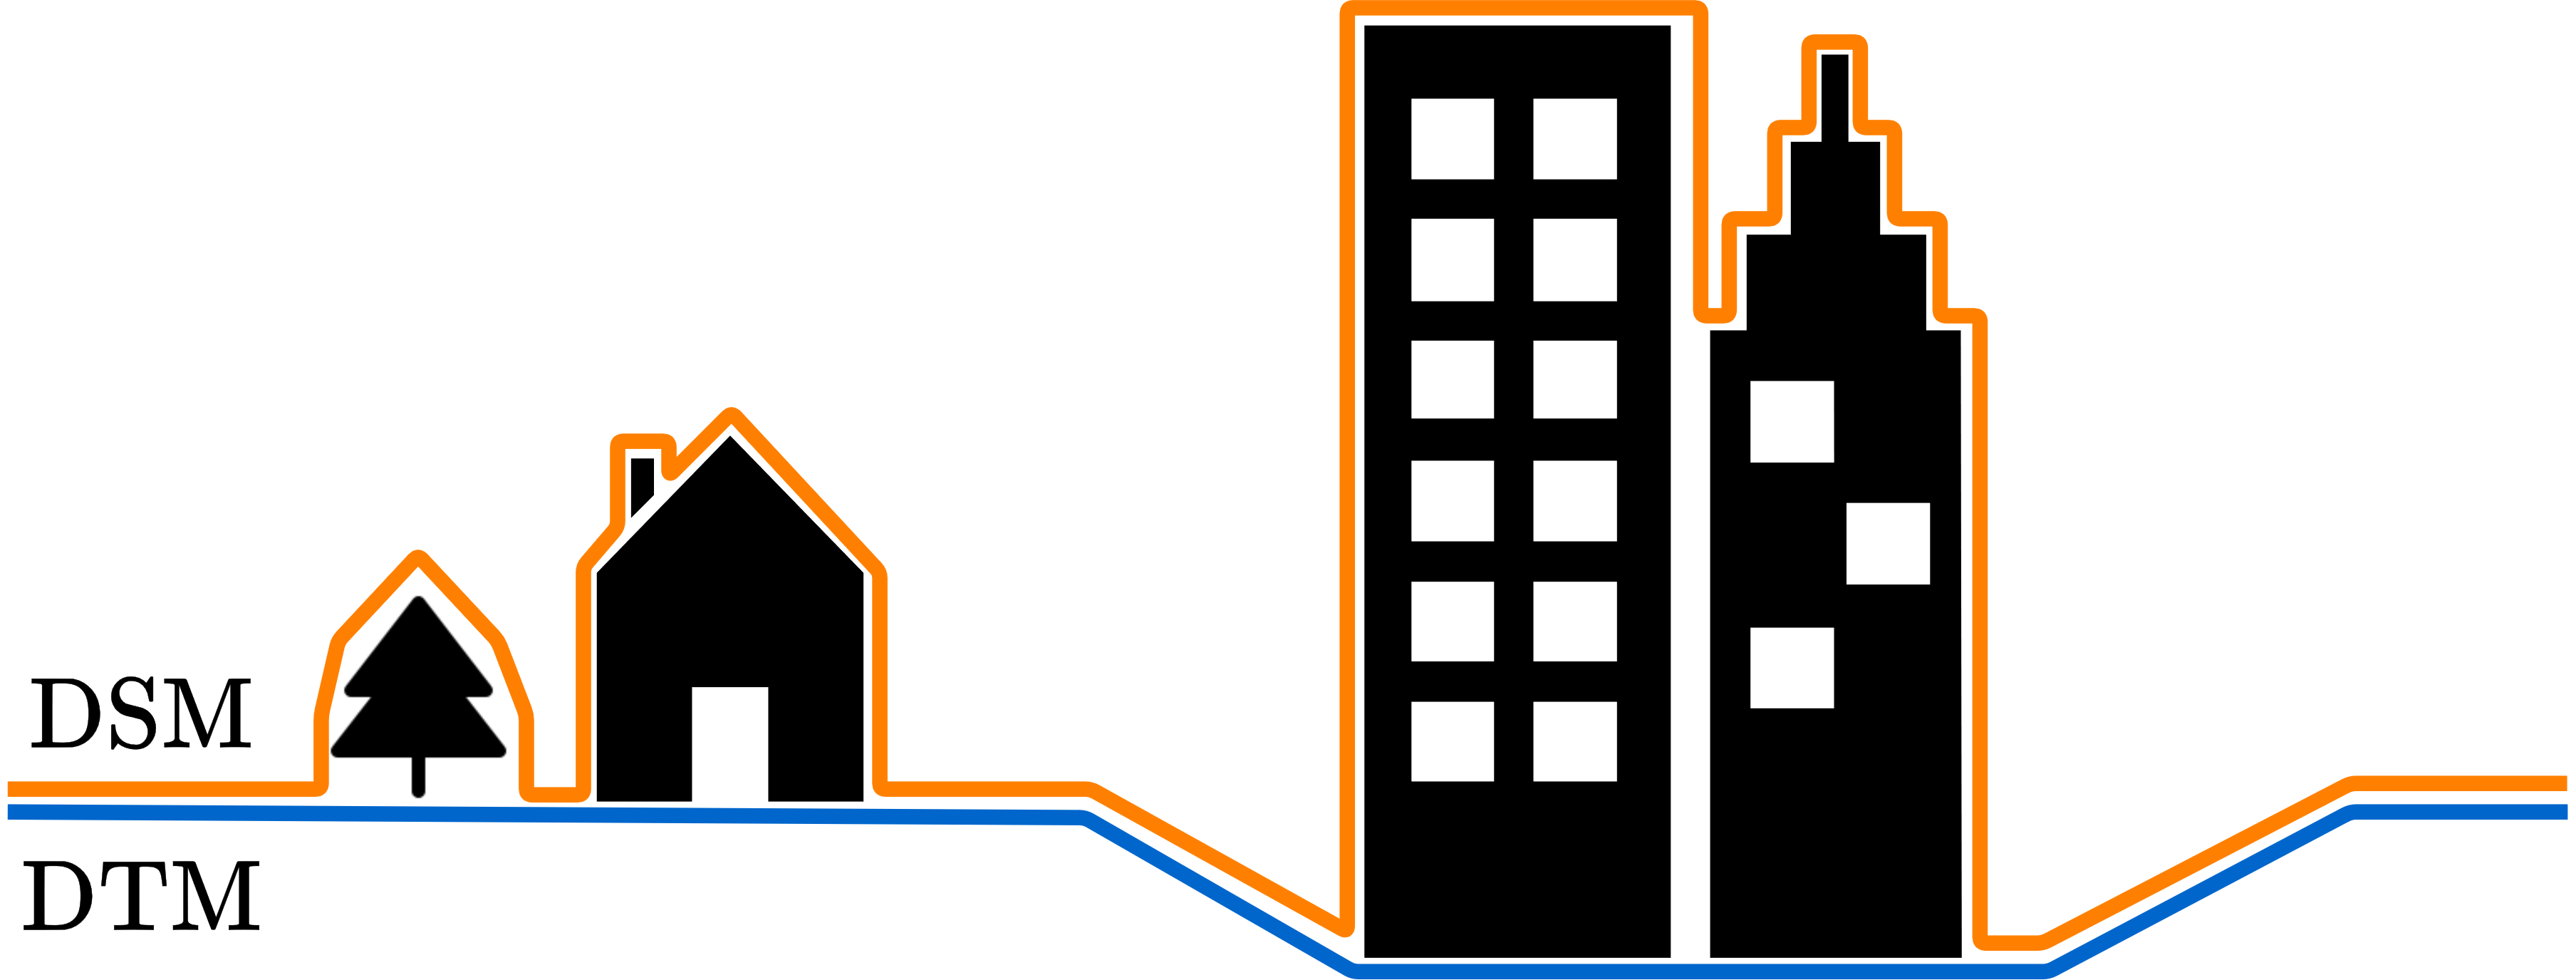
\includegraphics[width=0.8\linewidth]{Images/Chap_1/DTM_DSM.png}
    \caption{Difference between \acrlong{dtm} and \acrlong{dsm}}
    \label{fig:DTM_DSM}
\end{figure}

\acrshort{dtm}s are used for hydrology applications, such as for estimating water reservoirs \cite{yamazaki_merit_2019}, river flow \cite{miguez-macho_incorporating_2007}, global snow resources \cite{gascoin_theia_2019} or modeling potential flood \cite{yamazaki_regional_2014}. On the other hand, the high level of details of \acrshort{dsm}s are used to monitor changes in vegetation \cite{sadeghi_canopy_2016}, melting rates of glaciers \cite{berthier_glacier_2014, rieg_pleiades_2018}, changes in volcanoes \cite{ganci_data_2022} or to precisely map snow depth on mountainous terrain \cite{marti_mapping_2016}. In urban environment, \acrshort{dsm} allow to predict the potential damage caused by floods \cite{jenkins_physics-based_2023} or to do urban planning \cite{velazco_3d_2012}. For instance, possessing \acrshort{dsm}s on the same city but for different acquisition dates allow to measure the growth rate of the city \cite{warth_dsm-based_2019}, or damages caused by an earthquake \cite{erdogan_detection_2019} in-between acquisitions. \acrshort{dsm} are also crucial for ortho-rectifying image, \ie geometrically correcting the effects of distortions between the sensor and the terrain \cite{toutin_ortho-rectification_2012}. When capturing an optical image, the satellite is not necessarily right above its target, as illustrated in \Cref{fig:ortho_nadir}. However, if the image must be used as a background for a map, it is usually required that the image must be captured vertically, referred to as nadir, in order to be free of any perspective effect. \acrshort{dsm}s allow to reproject images as if they were taken at nadir. This rectification is used for many satellite products \cite{hagolle_maja_2017}.  
\begin{figure}
    \centering
    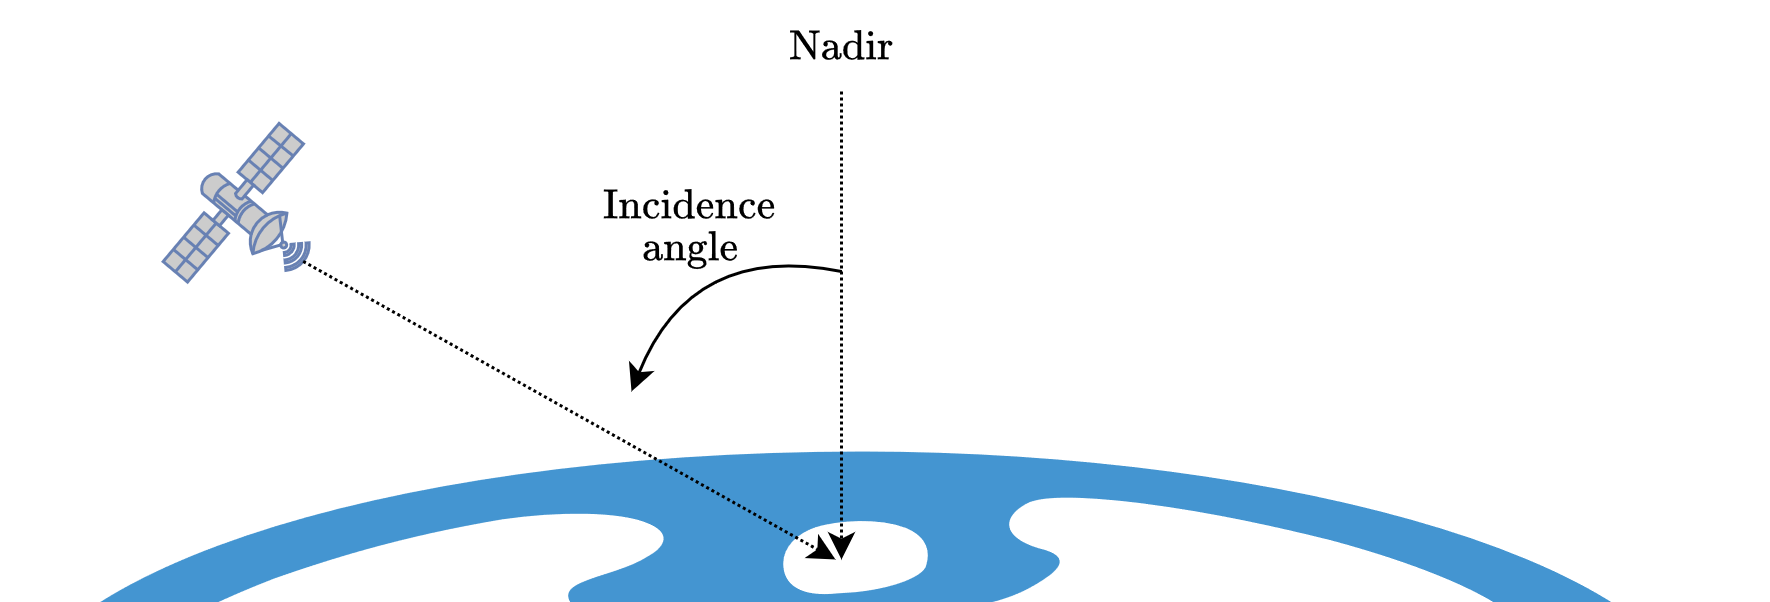
\includegraphics[width=0.7\linewidth]{Images/Chap_1/Ortho_Nadir.png}
    \caption{Incidence angle of a satellite, and nadir direction}
    \label{fig:ortho_nadir}
\end{figure}

Many applications depends on the resolution of \acrshort{dsm}s: evaluating water reservoirs in a mountainous regions does not necessarily require the same accuracy as 3D urban modelling for instance. The precision of a \acrshort{dsm} is defined by its planimetric resolution, \ie the size of a cell, and its altimetric resolution, \ie the smallest elevation variation it can detect. The altimetric resolution is itself characterized two notions: the absolute and relative accuracy. Absolute accuracy is the precision of a \acrshort{dsm} at a pixel level, \ie how close the predicted elevation is to the true elevation at the geographic coordinates of a given cell. Relative accuracy characterizes the quality of the 3D reconstruction of a scene. For instance, a \acrshort{dsm} precisely reproducing the shape of a house and its chimney will have a high relative accuracy. However, if the house is not properly georeferenced then the \acrshort{dsm} will have a poor absolute accuracy. Relative accuracy is therefore always greater than the absolute accuracy. In this thesis, we will mainly consider relative accuracy when evaluating the quality of \acrshort{dsm}s, as our sources possess different georeferencing systems which naturally induces small planimetric errors. 

There are multiple ways of creating a \acrshort{dsm} from airborne sensors such as planes, drones or satellites. The first way is to use \acrshort{radar} interferometry, as done by Sentinel-1 satellites \cite{geudtner_sentinel-1_2014} for instance. This method presents the advantage of being able to acquire data by day and night, even in the presence of clouds. Radar sensors, such as those present in the Shuttle Radar Topography Mission (SRTM) \cite{farr_shuttle_2007} or TanDEM-X \cite{krieger_tandem-x_2007}, possess a large swath of around $30$km, which was used to produce \acrshort{dsm}s covering the majority (or totality for TanDEM-X) of emerged land. The planimetric accuracy are in the range of a dozen meters (10m for TanDEM-X or 30m for the SRTM), and relative altimetric resolution is typically of a few meters (2m for TanDEM-X and 8m for the SRTM). This is not sufficient to distinguish objects such as buildings or trees, but rather global terrain topography. \Cref{fig:etoile_radar} presents a TanDEM-X \acrshort{dsm}. SRTM and TanDEM-X \acrshort{dsm} are not meant to be produced on a regular basis, and thus do not allow for temporal analysis as such. Another method for constructing \acrshort{dsm}s is to use stereophotogrammetry \cite{tao_comprehensive_2001}. Photogrammetry is the science of recovering 3D information from optical images. For this method, images of a scene are acquired from different points of view, and depth information is recovered from the parallax effect between images, already presented in \Cref{fig:parallax}. Photogrammetry is not restricted to the production of \acrshort{dsm}s, as it has many usages in robotics, for instance on Martian rovers \cite{goldberg_stereo_2002} or autonomous driving \cite{geiger_vision_2013}. Current optical satellites have a sub-meter resolution and a large swath (20km for Pléiades for instance \cite{coeurdevey_pleiades_2012}), allowing to massively produce high-resolution \acrshort{dsm} covering the globe for a relatively low cost using photogrammetry. The altimetric resolution is typically around one meter, although it depends of the different acquisition angles of the satellites. With this resolution, buildings, trees, and even cars can be detected on the \acrshort{dsm}. A final method for producing \acrshort{dsm} is to use \acrshort{lidar} (laser sensors) \cite{khosravipour_generating_2016}. Space-borne \acrshort{lidar}s are mostly used for atmospheric or discrete measurements \cite{fouladinejad_history_2019}. For instance, NASA’s ICESat-2 \cite{jasinski_atlasicesat-2_2020} measures elevation of seas and glaciers using 6 lasers taking measurements along track, which is not adapted for reconstructing high-accuracy DSM. On the other hand, planes or drones equipped with \acrshort{lidar} sensors usually have very good accuracy, allowing to model tower cranes, lamp post or small details on buildings. In particular, \acrshort{ign} uses \acrshort{lidar} to create point clouds with a planimetric accuracy of 25 centimeters and an altimetric resolution of 5 centimeters, and then produce \acrshort{dsm}s out of it  \cite{monnet_lidarhd_2023, ign_lidar_2024}. This is part of a 5 years campaign named \acrshort{lidar} HD and started in 2021, where planes equipped with \acrshort{lidar} sensors will cover the whole French territory (except French Guiana). Those types of campaign are long and costly, and can hardly be reproduced at a global scale. Therefore, photogrammetry \acrshort{dsm}s are currently the best solution to produce \acrshort{dsm}s covering the globe, with a sub-meter resolution for relatively low costs. \Cref{fig:etoile} presents examples of \acrshort{dsm}s produced by \acrshort{radar}, photogrammetry and \acrshort{lidar}.

\begin{figure}
    \begin{subfigure}[t]{0.31\linewidth}
        \flushleft
        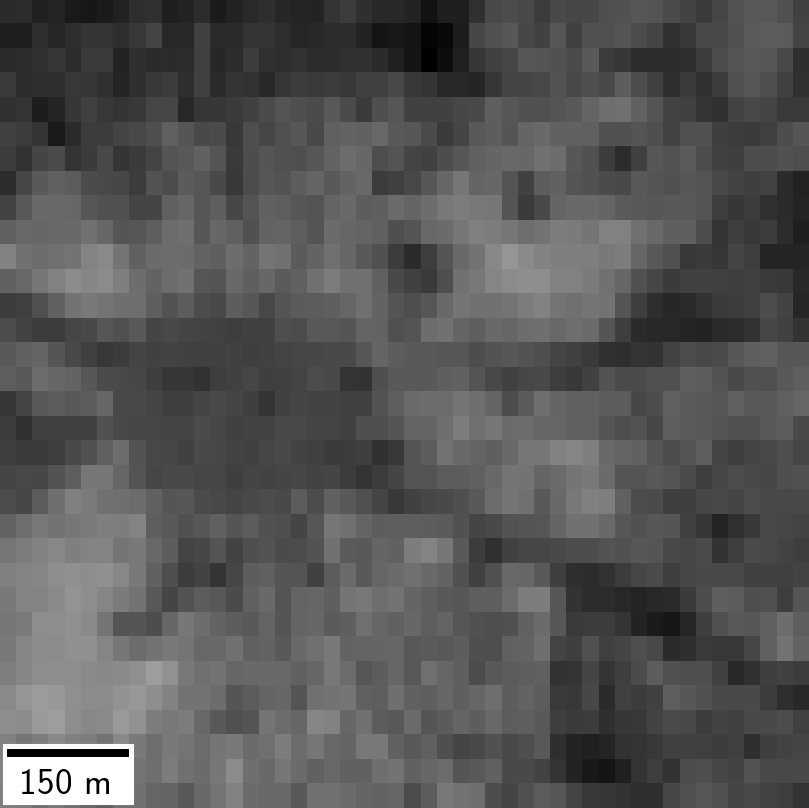
\includegraphics[width=\linewidth]{Images/Chap_1/etoile_low_res_dsm.png}
        \caption{\acrshort{radar} \acrshort{dsm}}
        \label{fig:etoile_radar}
    \end{subfigure}\hfill
    \begin{subfigure}[t]{0.31\linewidth}
        \centering
        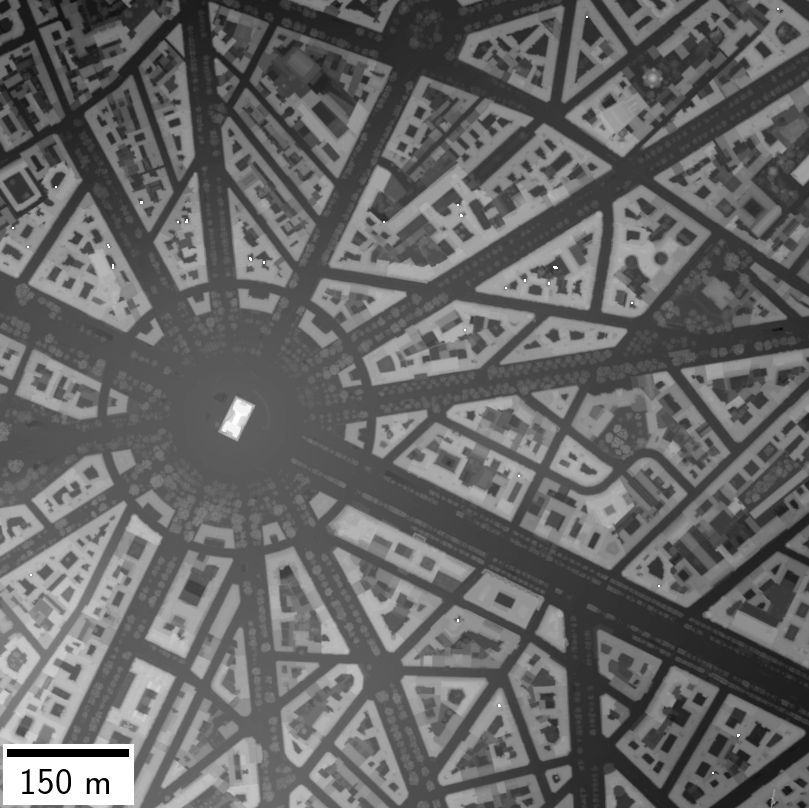
\includegraphics[width=\linewidth]{Images/Chap_1/etoile_high_res_dsm.png}
        \caption{\acrshort{lidar} \acrshort{dsm}}
        \label{fig:etoile_lidar}
    \end{subfigure}\hfill
    \begin{subfigure}[t]{0.365\linewidth}
        \flushright
        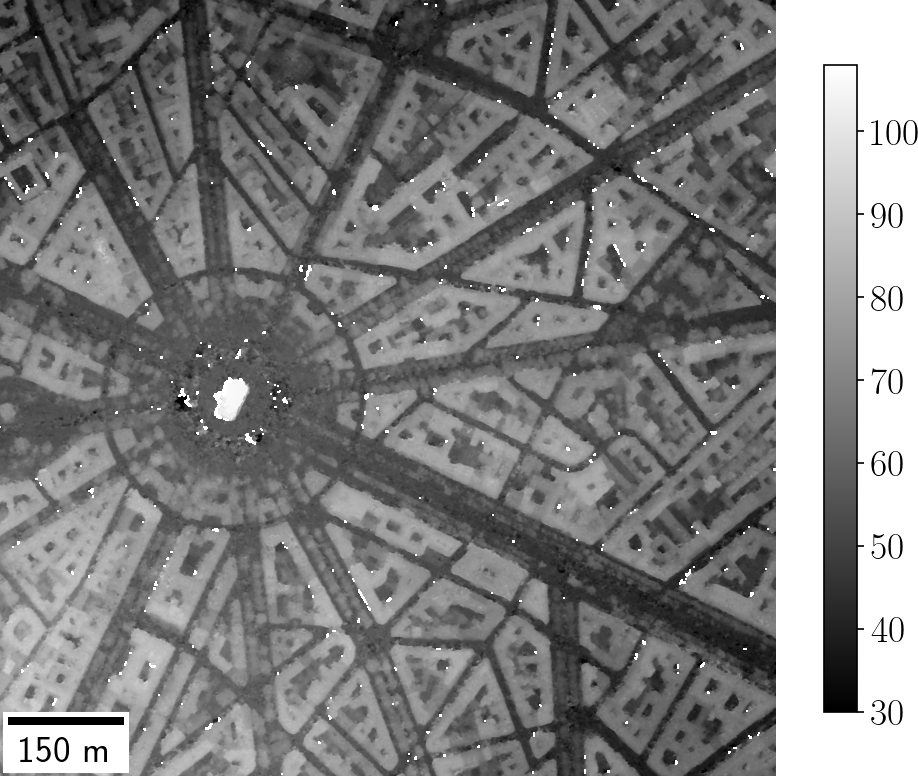
\includegraphics[width=\linewidth]{Images/Chap_1/etoile_cars_dsm.png}
        \caption{Photogrammetry \acrshort{dsm}}
        \label{fig:etoile_photogrammetry}
    \end{subfigure}
    \caption{\acrshort{dsm}s over Arc de Triomphe, Paris, obtained with different sensors.}
    \label{fig:etoile}
\end{figure}

In this thesis, we use \acrshort{lidar} \acrshort{dsm} as our reference \acrshort{dsm}s due to their high quality. They will be used to evaluated the errors or uncertainties of \acrshort{dsm}s produced using stereophotogrammetry. The next section details which stereo images we will be using to produce those \acrshort{dsm}s. 

\section{Satellite Photogrammetry}\label{sec:co3d}
This section presents the different sensors, satellites and geolocation models that will be used to acquire and process stereo images.

\subsection{Different sensors}
Different types of sensors can be used to acquire optical satellite images. We detail in this section a (non-exhaustive) list of sensors of interest \cite{cnes_imagerie_2008}.

\subsubsection{Push-broom sensor}
For each observed wavelength, push-broom sensor are only composed of a single cell row, acquiring simultaneously radiometric information alongside a line perpendicular to the direction of the satellite. We use the satellite movement along track to acquire the different rows of the image, as seen in \Cref{fig:ccd_pushbroom_sensors}. As only one line of cells is needed, push-broom sensors are simple systems which can capture images continuously, while guarantying good geometrical quality along the rows of the images. A variation of those sensors are TDI sensors (Time Delay Integration). Those sensors function as a push-broom except that each row has the ability to transfer its photon charges to the next row. This allows to capture signals over a longer period of time,  thus reducing the signal-to-noise ratio. Harder to produce, TDI sensors also require a precise control of the satellite so that observed objects stay within a column of the TDI sensor. 

\subsubsection{CCD sensors}
\acrfull{ccd} are classical sensors, used in current digital cameras for instance. They consist of a grid of cells sensitive to a given wavelength configured in a checkerboard pattern. A specific type of \acrshort{ccd} sensors are Bayer matrices, where the sensor only possesses a single type of photo-sensitive cell and the different colors are captured by applying a color filter on the sensor. \acrshort{ccd} sensor possess multiple advantages, such as good geometrical quality as all pixels are acquired simultaneously, or the possibility to perform many acquisitions with various angles possible. \acrshort{ccd} sensors are relatively recent in spatial imagery as they are technologically difficult to built. Augmenting the number of pixels complicates the shutter function and occupies more space compared to push-broom sensors. It requires more radiometric calibration as each pixel results from a different photo-sensitive cell. Acquire long segments of an image is not natural as it is the case for push-broom sensors.

\begin{figure}
    \begin{subfigure}[t]{0.5\linewidth}
        \centering
        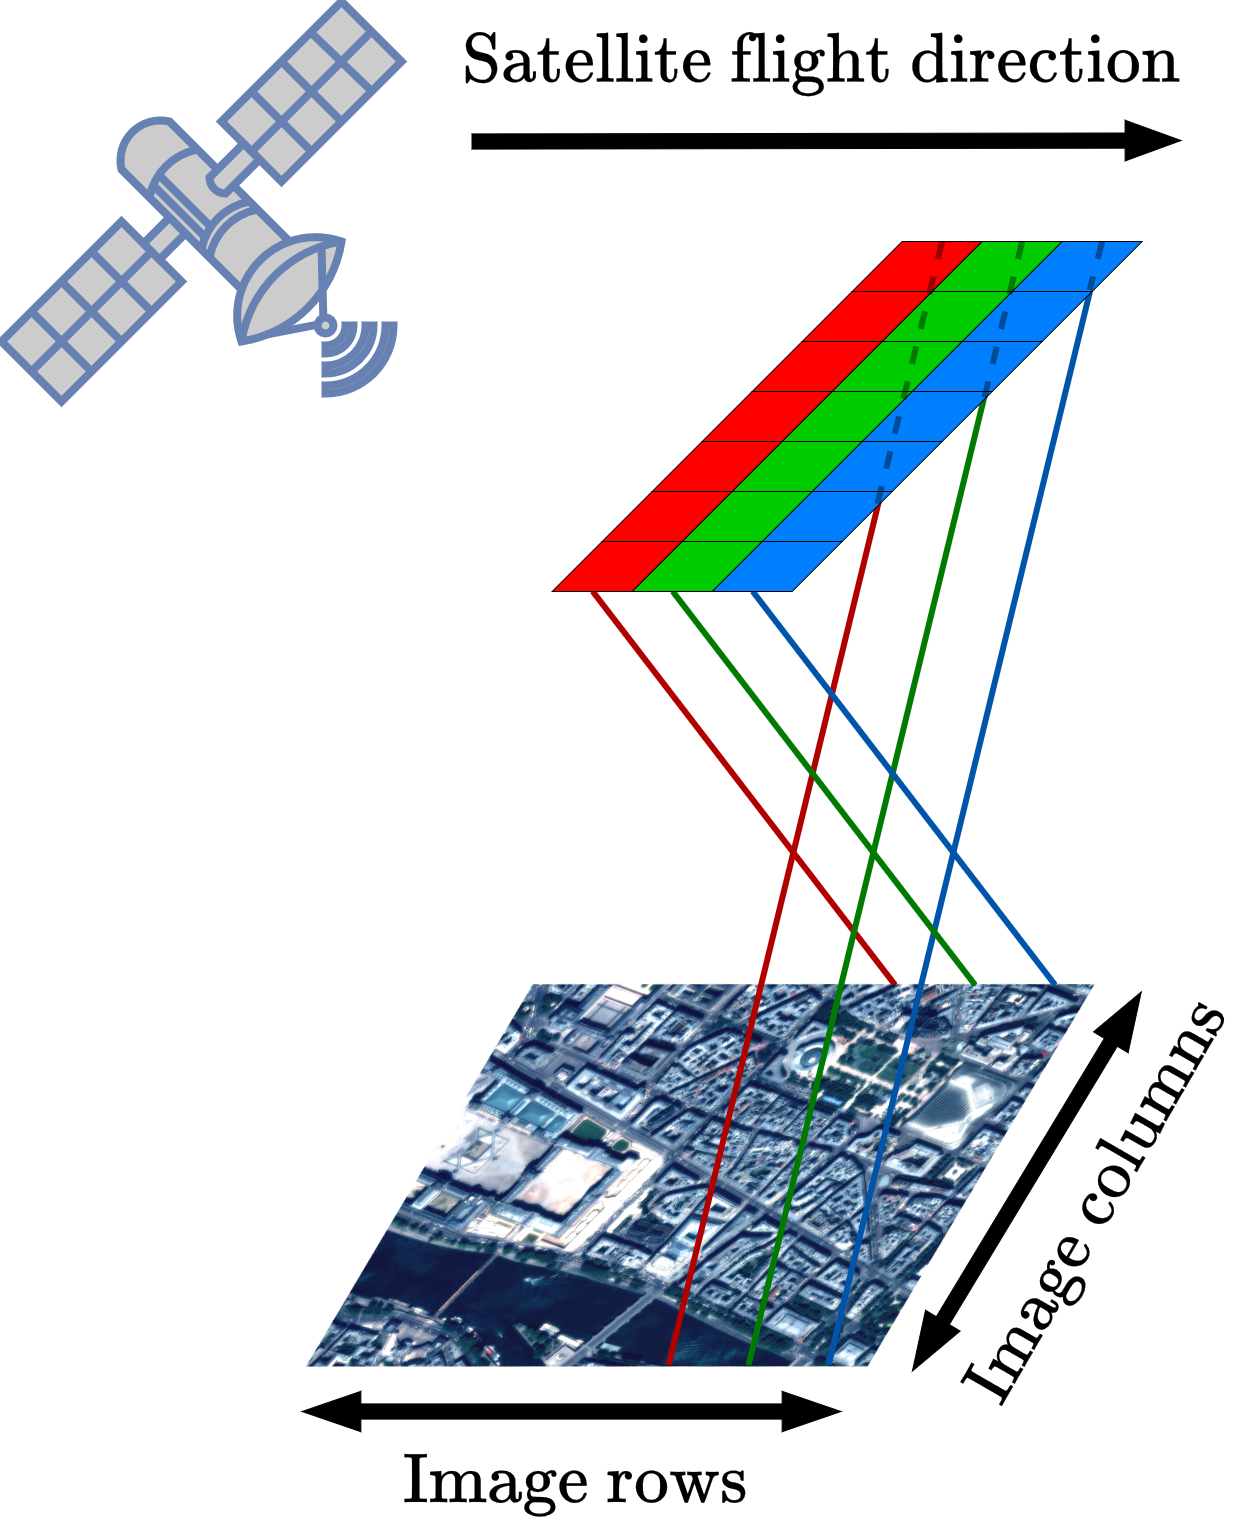
\includegraphics[height=6cm]{Images/Chap_1/pushbrrom.png}
        \caption{Push-broom sensor}
        \label{fig:pushbroom}
    \end{subfigure}
    \begin{subfigure}[t]{0.5\linewidth}
        \centering
        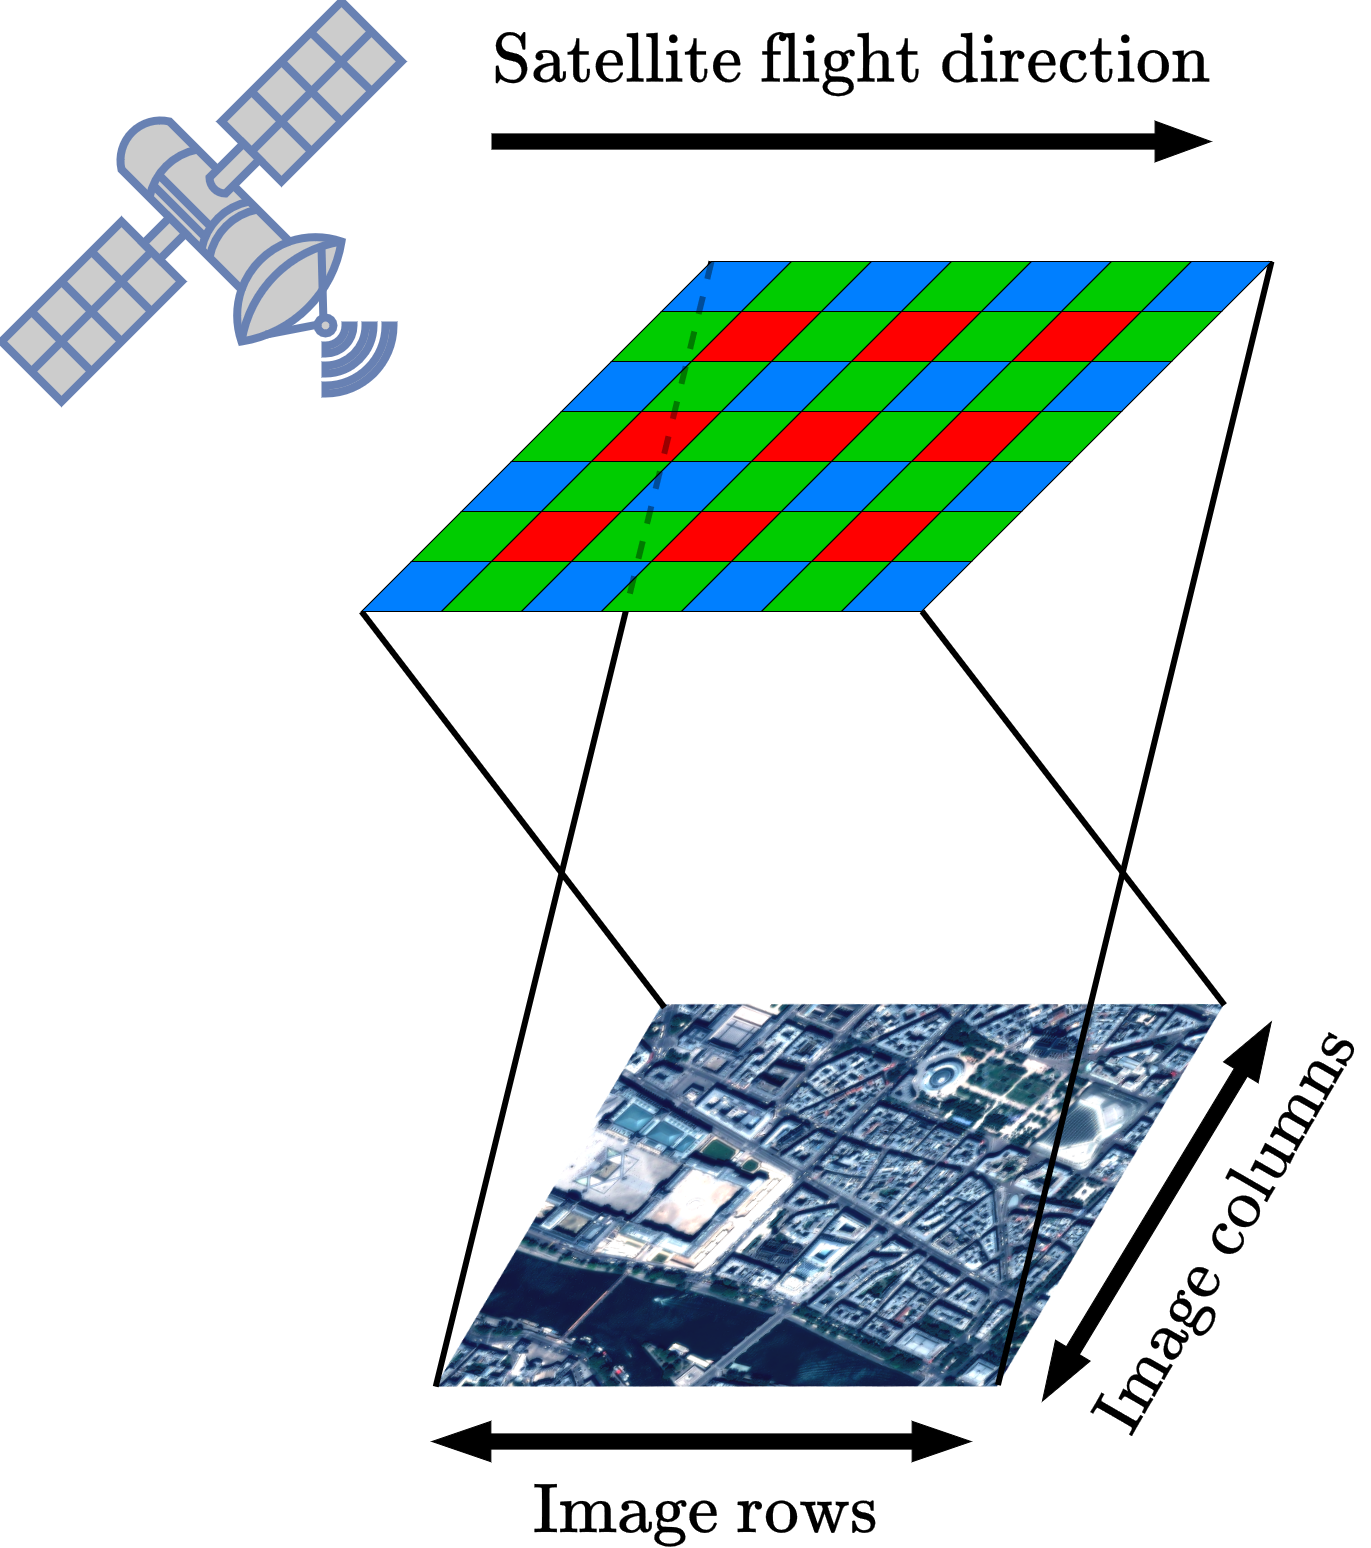
\includegraphics[height=6cm]{Images/Chap_1/CCD.png}
        \caption{\acrshort{ccd} sensor}
        \label{fig:ccd}
    \end{subfigure}
    \caption{Schematic representation \acrshort{ccd} and push-broom sensors}
    \label{fig:ccd_pushbroom_sensors}
\end{figure}

Those different sensors are used in most \acrfull{vhr} optical satellites as we will see in the next section.

\subsection{VHR satellites}
In this section, we present different \acrshort{vhr} optical satellites which can be used to acquire stereo images. 

Across the years, different constellations of \acrshort{vhr} satellites have been launched, either for civilian (SPOT 1-7), defense (CSO) or commercial use (Ikonos, QuickBird, Worldview 1-3). Most of them are agile satellites, using push-broom sensors that can now reach resolutions near 30cm \cite{cnes_imagerie_2008, coffer_vertical_2022}. One constellation of interest that we will consider in this thesis is the Pléiades constellation. Developed by Airbus, this constellation is composed of two identical satellites, 1A and 1B. The satellites were launched in 2011 and 2012 in an helio-synchronous orbit at $690$km, for both civilian and defense usages. They provide panchromatic images at a resolution of $70$cm (resampled at $50$cm), and \acrshort{rgb}-\acrshort{nir} images at a resolution of $2$m, with a $20$km swath (\url{https://dinamis.data-terra.org/pleiades/}) using a push-broom TDI sensor. Their high agility and revisit rate allow them to capture stereo and tri-stereo images for any location on the globe, ideal to produce \acrshort{dsm} with high accuracy. \Cref{fig:Pleiade_over_Paris} provide an example of a Pléiades stereo acquisition. A ``video'' mode is even available were dozens of image of the same scene can be acquired in the span of a few minutes \cite{lebegue_pleiades-hr_2015}. However, stereo acquisitions is not the only objective of this mission, even though the demand for those products is increasing \cite{berthier_glacier_2014, poli_radiometric_2015, rieg_pleiades_2018, loghin_potential_2020}. The acquisition of stereo images is thus provided on command, which can conflict with other usages of the satellite, and can become costly when trying to cover large areas. Pléiades is also a satellite for both defense and civilian usages, military acquisitions having the priority over civilian one. Pléiades acquisitions can also be requested using the ``Disaster Chart'' (\url{https://disasterscharter.org/fr/web/guest/home}) in order to evaluate damages caused by floods, landslide or earth quakes for instance, and to better plan and provide emergency relief to victims of those disasters.

\begin{figure}
    \centering
    \begin{subfigure}[t]{0.5\linewidth}
        \centering
        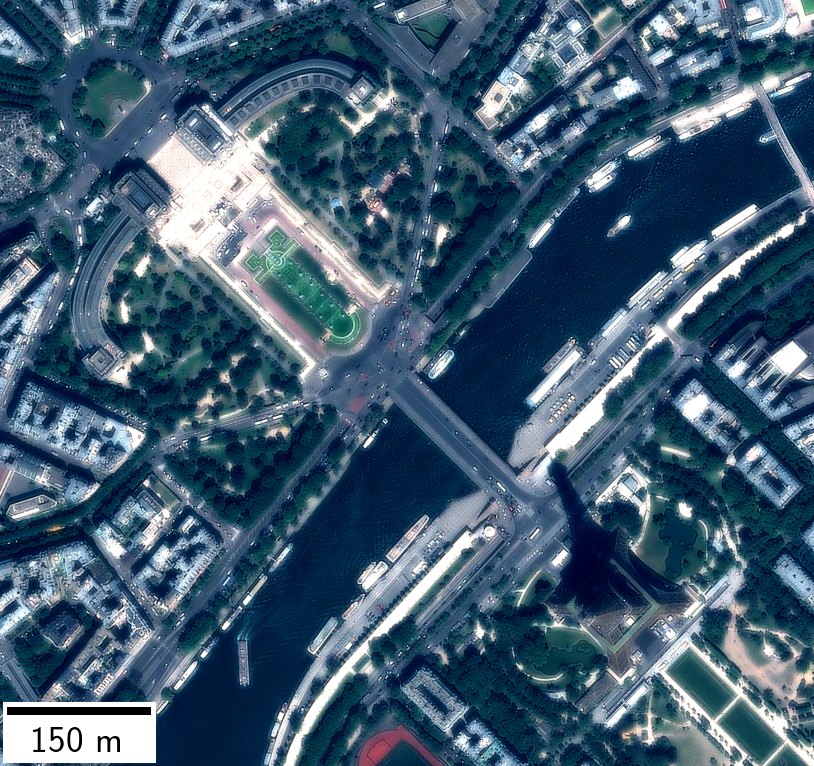
\includegraphics[height=6cm]{Images/Chap_1/Paris_Left_stereo.png}
        \caption{Left image}
        \label{fig:Pleiade_over_Paris_a}
    \end{subfigure}\hfill
    \begin{subfigure}[t]{0.5\linewidth}
        \centering
        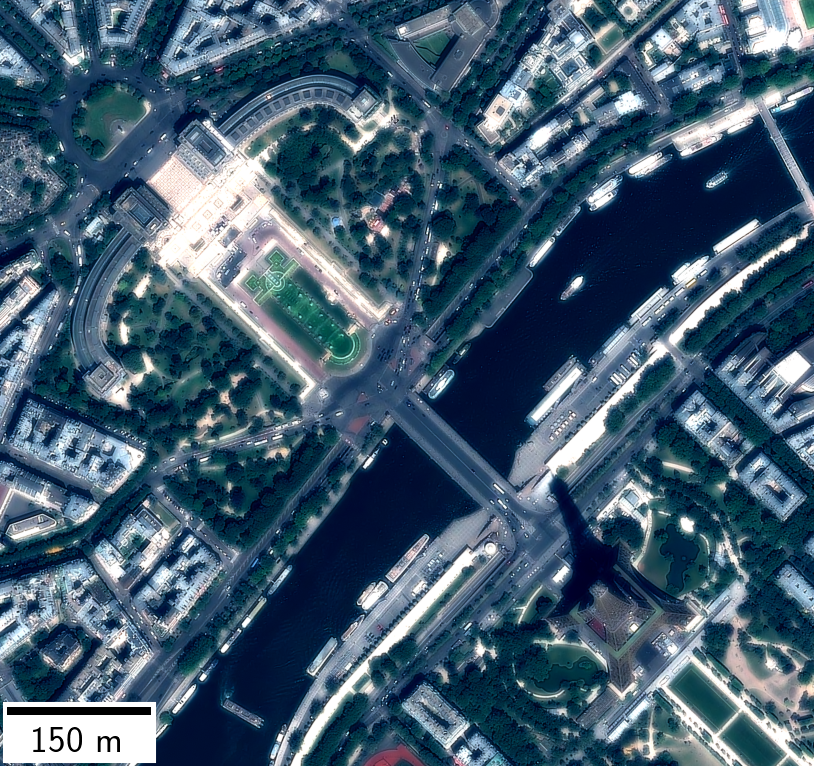
\includegraphics[height=6cm]{Images/Chap_1/Paris_Right_stereo.png}
        \caption{Right image}
        \label{fig:Pleiade_over_Paris_b}
    \end{subfigure}
    \caption{Pansharpened Pléiades stereo images over Paris at $0.5$m of resolution. The change of point of view can be easily observed by looking at the Eiffel Tower. Pléiades \copyright \acrshort{cnes} 2023, Distribution AIRBUS DS}
    \label{fig:Pleiade_over_Paris}
\end{figure}

In order to produce a worldwide \acrshort{dsm} with $1$m resolution by 2025, the \acrfull{cnes} is launching the \acrfull{co3d} mission \cite{melet_co3d_2020}. Composed of two pairs of low-cost satellites (\Cref{fig:co3d_mission}) equipped with \acrshort{vhr} optical sensors, the mission will produce image in the \acrshort{rgb} and \acrshort{nir} spectrum at $0.5$m of resolution \cite{lebegue_co3d_2020} using a \acrshort{ccd} sensor cell, and more specifically a Bayer matrix. The pairing of satellites and \acrshort{ccd} sensor used allow for \textit{almost} simultaneous stereo image acquisition, cutting short the transient object problem (\ie objects moving/disappearing between stereo images). To be able to process the amount of data provided by the \acrshort{co3d} mission ($40\,000$ images a day, at $50$cm resolution and covering a footprint of 7km$\times$5km \cite{melet_co3d_2020, lebegue_co3d_2020}), every step of the pipeline has been developed to be highly scalable. Different acquisition schemes can also be used, such as the video mode, or even the `diamond' geometry acquisition, which acquires a quadri-stereo over a couple of days. In parallel with image quality specifications, the \acrshort{co3d} products need to abide to a height relative accuracy of $1$m on low slopes. In addition, the \acrshort{co3d} mission plans to produce a performance map supporting the output DSM. Therefore, investigating uncertainty inside a 3D stereo pipeline is essential for the implementation of this performance map.

\begin{figure}
    \centering
    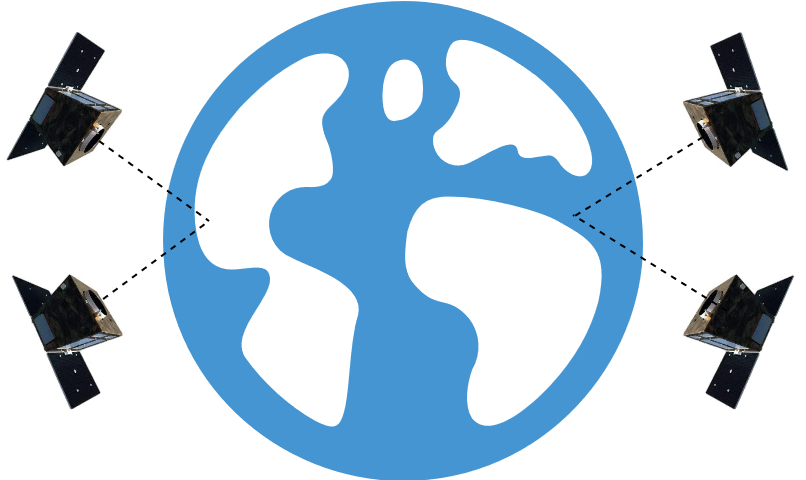
\includegraphics[width=0.6\linewidth]{Images/Chap_1/CO3D_schema.png}
    \caption{Pairing of satellites for the \acrshort{co3d} mission. (Credit: \acrshort{cnes})}
    \label{fig:co3d_mission}
\end{figure}

\begin{remark}
    When an image is acquired both in panchromatic and RGB mode, it is possible to leverage the high resolution of the panchromatic image to improve that of the color image. This fusion technique is called \textit{pansharpening} \cite{loncan_hyperspectral_2015}. We use this technique for clarity in figures and other illustrations of this thesis (for instance \Cref{fig:VDG_ortho,fig:Pleiade_over_Paris}). It is important to remember that the processed images are the panchromatic images, and not the pansharpened ones which are only used for the final visualization. The \acrshort{co3d} satellites are not concerned with pansharpening, as the used Bayer matrix directly provides \acrshort{rgb} images at 50cm resolution without panchromatic band.
\end{remark} 

Although this thesis contributes to the ground segment of the \acrshort{co3d} mission, we used Pléiades stereo images in the absence of \acrshort{co3d} images (at the time this thesis is written, the \acrshort{co3d} mission has not yet been launched).

\subsection{Geolocation Models}\label{sec:sensors_rpc}
A crucial part of satellite imagery is the ability to perform georeferencement, or georegistratation, of every pixel, \ie, locate their coordinates in an Earth system of coordinates.

Different systems of coordinate exist, for instance the Geodetic Coordinates use latitude and longitude to represent the relative position of a point with regards to a reference ellipsoid, \ie a smooth and regular mathematical approximation of the Earth's shape. Another widely used reference system is the \acrfull{utm} coordinate system, which divides the globe into sixty north-south areas. Each area is $6\degree$ of longitude wide, and is approximated by a plane. The coordinates of a point in each area are Cartesian coordinates with the origin being the intersection of the equator and the meridian of the area. \acrshort{utm} coordinates are employed in GPS systems for instance. In Geodetic Coordinates or \acrshort{utm}, the elevation of a point is defined using the ellipsoid as reference. It is also possible to use the geoid, \ie the gravity equipotential surface, which is less smooth than the ellipsoid but is closer to the actual irregular shape of the Earth.

Physical models possess high geolocation accuracy, but are sensor-specific and are computationally complex. For stereo reconstruction, generalized sensor models are preferred. Specifically, we will focus on \acrfull{rpc}, provided alongside images of many satellites \cite{grodecki_ikonos_2001,devika_developement_2006}, and specifically of the \acrshort{co3d} and Pléiades satellites. Sometimes called Polynomial Mapping Functions \cite{baltsavias_metric_1992} or Rational Function Models \cite{tao_comprehensive_2001}, \acrshort{rpc} are functions allowing to transform a pixel's ground location in Geodetic Coordinates, \ie its longitude, latitude and geodetic height $(X,~Y,~Z)$, into its coordinates $(\rowcol)$ in the image space. \acrshort{rpc} encode lines of sight of the satellite, \ie the line joining the center of the sensor's cell to the ground and going through the optical center of the sensor. To improve numerical stability and minimize computation errors, the image coordinates and ground coordinates are normalized between $-1$ and $1$, using their scale factors $SF$ and mean values:
\begin{eqnarray*}
    SF_X &=& \max(X_\mathrm{max}-\overline{X},~\overline{X}-X_\mathrm{min})\\
    \Tilde{X}&=&\frac{X-\overline{X}}{SF_X}
\end{eqnarray*}
The same process is applied to $Y, ~Z,~row$ and $col$. To avoid heavy notation in this section, we will refer to every normalized coordinate using their non-normalized symbol.

\begin{figure}
    \centering
    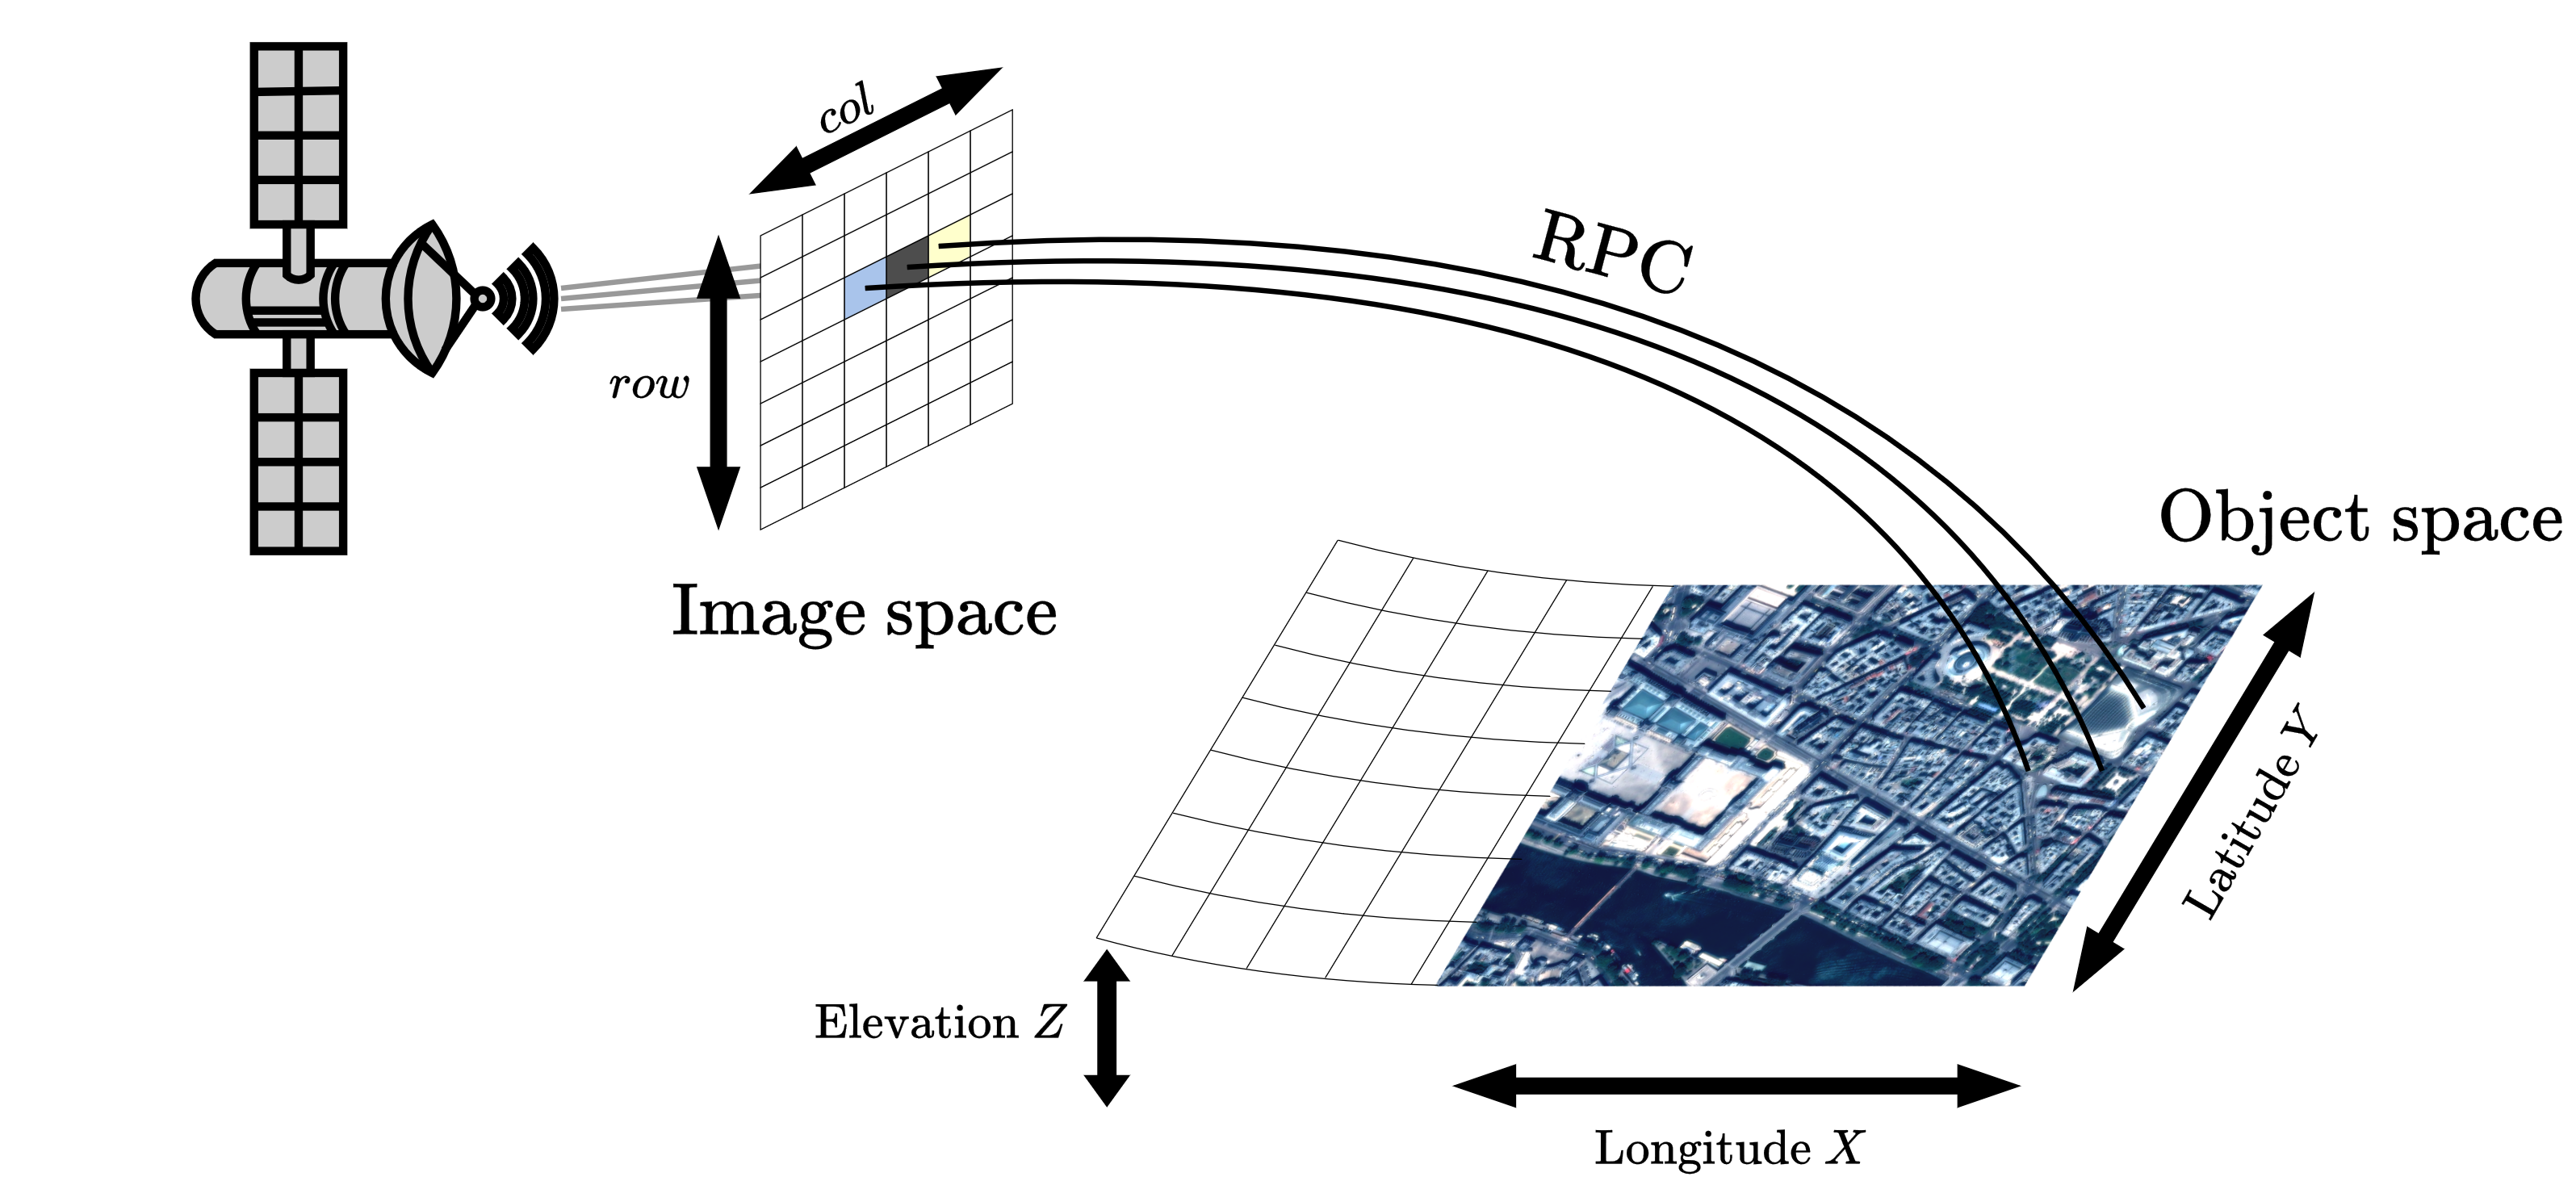
\includegraphics[width=0.8\linewidth]{Images/Chap_1/RPC_model.png}
    \caption{Schematic representation of \acrshort{rpc} models.}
    \label{fig:RPC_models}
\end{figure}

Formally, \acrshort{rpc} are defined as rational fractions of polynomials:  
\begin{eqnarray}
    \RPC:\mathbb{R}^3 &\rightarrow&\mathbb{R}^2\nonumber\\
    (X,~Y,~Z) 	&\mapsto& \left(\frac{Num_{row}(X,Y,Z)}{Den_{row}(X,Y,Z)}, \frac{Num_{col}(X,Y,Z)}{Den_{col}(X,Y,Z)}\right)\nonumber\\
    &\mapsto&(row,col)\label{eq:rpc}
\end{eqnarray}
where $Num_{row},~Den_{row},~Num_{col}$ and $Den_{col}$ are the numerators and denominators for rows and columns respectively, expressed as polynomials with a maximum order of $3$:
\begin{eqnarray*}
    Num_{row}(X,~Y,~Z) &=& \sum_{i=0}^3~\sum_{j=0}^{3-i}~\sum_{k=0}^{3-i-j}a_{ijk}X^iY^jZ^k\\
    &=& a_{000} + a_{100} X + a_{010} Y + a_{001} Z + a_{110} XY + a_{101} XZ \\
    &&+ a_{011} YZ + a_{200} X^2 + a_{020} Y^2 + a_{002} Z^2 + a_{111} XYZ \\
    && + a_{210} X^2Y + a_{201} X^2Z + a_{120} XY^2 + a_{102} XZ^2\\
    && + a_{021} Y^2Z + a_{012} YZ^2 + a_{300} X^3 + a_{030} Y^3 + a_{003} Z^3
\end{eqnarray*}
$Den_{row},~Num_{col}$ and $Den_{col}$ respectively possess different coefficients $a_{ijk}$. The order or indexing of $a_{ijk}$ may differ in the literature. For instance, they can be numbered from $0$ to $19$ or $1$ to $20$, and do not refer to the same indeterminate. Numerical values of \acrshort{rpc} coefficient are computed using a set of reference ground control points.

It has been shown in \cite{baltsavias_metric_1992} that \acrshort{rpc} are well suited to be used for ortho-rectification and stereophotogrammetry, as they possess good accuracy and are computationally fast. For stereophotogrammetry, it is often required to use the inverse \acrshort{rpc} model. As \acrshort{rpc} encode a line of sight given an image coordinate, the use of an additional elevation coordinate is required to move from the image space to the object space (\ie to go from a 2D space to a 3D space). It can be a geoid modelling the Earth's surface, or a \acrshort{dsm} with higher resolution. Knowing the true elevation $Z$ of a pixel, we define the inverse model as:
\begin{eqnarray}
    \RPC^{-1}:\mathbb{R}^3 &\rightarrow&\mathbb{R}^3\nonumber\\
    (\rowcol,~Z) 	&\mapsto& (X,~Y,~Z) \label{eq:inverse_rpc}
\end{eqnarray}
An illustration on how \acrshort{rpc} can be used to go from the image space (\rowcol) to the object space $(X,Y,Z)$ is presented in \Cref{fig:RPC_models}. Knowing the position of pixels in the object space using \acrshort{rpc} allows to triangulate the position of an object using multiple images of the same scene. This is how photogrammetry pipelines processing satellite images are computing the elevation of the different cells of a \acrshort{dsm}. The next section will explain the inner workings of those pipelines.

\section{Structure of the Stereophotogrammetry Pipeline}\label{sec:classical_stero_pipeline}
This section dives more into details of the inner workings of stereophotogrammetry, and presents the stereo pipeline mainly considered in this thesis. Photogrammetry is the science of deducing information from photographic images \cite{kasser_photogrammetrie_2001}. A sub domain of photogrammetry is stereophotogrammetry, which specifically consists in deducing 3D information from multiple photographic images. Although multiple stereophotogrammetry setups can be achieved, for instance using structured light \cite{scharstein_high-accuracy_2003} or different wavelength \cite{geng_rainbow_1996}, we focus here on the pipelines designed for processing satellite images, which are used and studied in this thesis. 


\begin{figure}
    \begin{subfigure}[t]{0.5\linewidth}
        \flushleft
        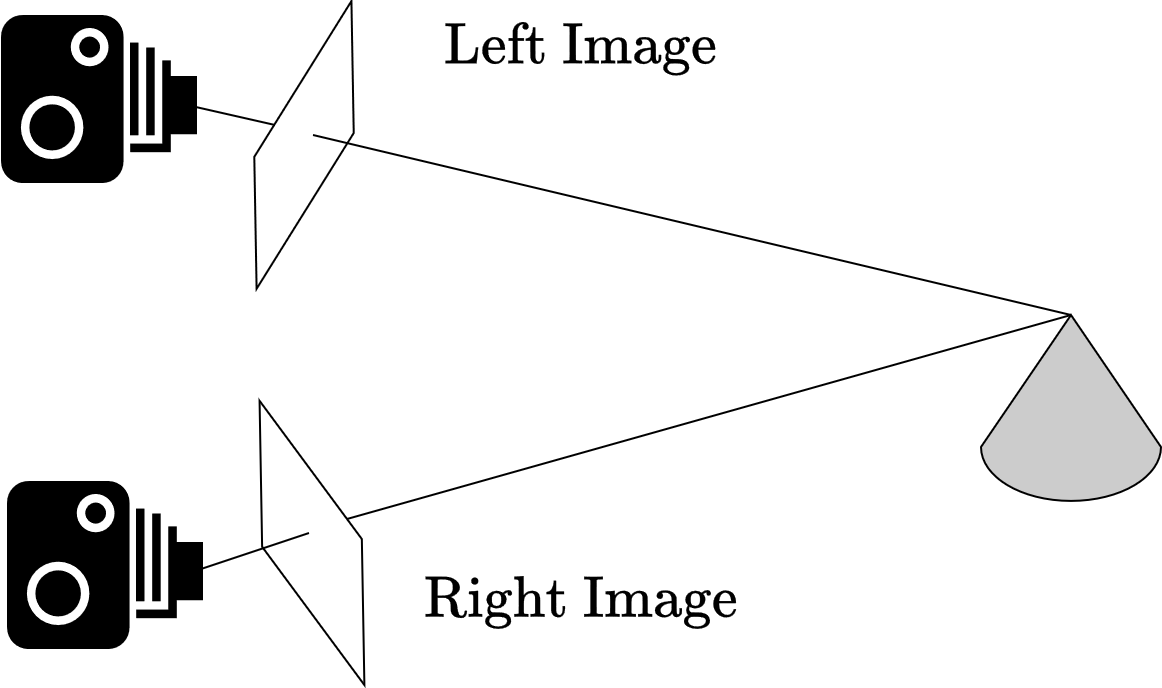
\includegraphics[width=0.7\linewidth]{Images/Chap_1/Sterero_principle_1.png}
        \caption{}
        \label{fig:stereo_principle_1}
    \end{subfigure}
    \begin{subfigure}[t]{0.5\linewidth}
        \flushright
        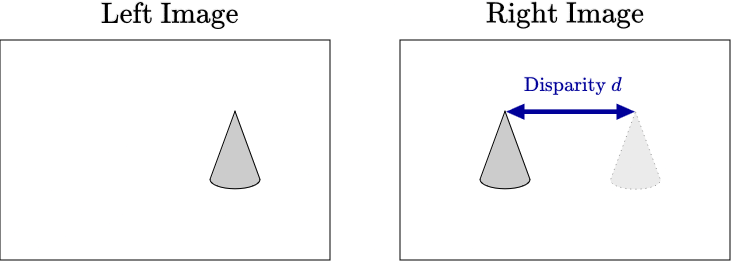
\includegraphics[width=\linewidth]{Images/Chap_1/Sterero_principle_2.png}
        \caption{}
        \label{fig:stereo_principle_2}
    \end{subfigure}
    \caption{Principle of photogrammetry. The same object is captured by two different cameras in \Cref{fig:stereo_principle_1}. The position of the object in both image spaces in \Cref{fig:stereo_principle_2}, is characterized by its displacement, called \textit{disparity}.}
    \label{fig:stereo_principle}
\end{figure}

The main idea of stereophotogrammetry is to identify the parallax of objects between multiple images, and to deduce the distance between the object and the sensors from this displacement. \Cref{fig:stereo_principle} illustrates how the position of an object can be triangulated from multiple images of a scene. The two lines of sight used to triangulate the position of an object are determined by finding the location of the object in both image spaces. Given the coordinate of an object in a reference image space (for instance the left image in \Cref{fig:stereo_principle}), the corresponding line of sight in the second image is completely determined by the position of the object in the reference image space, and its displacement between the two images spaces. When expressed in pixels, this displacement is called disparity, as presented in \Cref{fig:stereo_principle_2}. Determining the disparity of every pixel of a reference image is called dense-matching, and is done by a dense-matching algorithm, also called \textit{correlator} (as it computes the best correlation between pixels of stereo images). It allows to create pairs of pixels representing the same object in their respective image space. Using the geometrical model of the camera, or the geolocation model of sensors in the case of satellite imagery, the 3D coordinates of the corresponding object of a pair of matched pixels can then be determined by intersecting lines of sight (or best approximation if they do not strictly intersect). This results in a point cloud, encoding the 3D position of every visible object in both images. In satellite photogrammetry, the point cloud can be projected onto a regular grid to obtain a \acrshort{dsm}. The following section dives more into details of satellite photogrammetry pipelines, and specifically on the \acrshort{cars} stereo pipeline.

\subsection{Different Photogrammetry Pipelines}\label{sec:different_photogrammetry_pipelines}
Several stereo pipelines processing satellite images exist in the literature. We can think of NASA's \textit{ASP} \cite{shean_automated_2016}, Centre Borelli's \textit{s2p} \cite{franchis_automatic_2014}, DLR's \textit{CATENA} \cite{kraus_fully_2013}, Ohio State University's \textit{RSP} and \textit{SETSM} \cite{qin_rpc_2016, noh_surface_2017}, \acrshort{ign}'s \textit{MicMac} \cite{rupnik_micmac_2017}. Concerning MicMac, we only consider the methods for satellite photogrammetry, as many other photogrammetry applications and methods are available in this software. For a comparison of those pipelines performances, we refer to \cite{bosch_metric_2017,qin_quality_2021}.

All those pipelines roughly possess the same structure:
\begin{itemize}
    \item Pre-processing. All those pipeline (except S2P) undergo a bundle adjustment step to refine images geometries and correct sensors misalignment.
    \item Images resampling in a convenient geometry for pixel matching. Most pipelines proposes multiple geometries for the resampling of images: the matching can directly be done in the object space, or the secondary image is compute in the geometry of the reference images, or both images are resampled into an epipolar geometry, \ie a geometry where objects move horizontally in both image spaces.
    \item Dense matching. RSP and S2P restrict the choice of the geometry to the epipolar geometry and therefore only propose to do 1D (row-wise) dense matching. Other pipeline allow for a 2D matching.
    \item Triangulation of matches to get 3D point clouds.
    \item Rasterization. When working with more than two images, pipelines all offer the possibility to fuse the obtained pair-wise \acrshort{dsm}s to obtain a global \acrshort{dsm}.
\end{itemize}
It is also noteworthy that when working with more than two images, only MicMac and ASP allow to consider all images at once, while other pipelines use multiple pairings of images. The way those pipeline handle uncertainty will be detailed in section \Cref{sec:related_work}.

We will focus on the \acrshort{cars} pipeline used in this thesis, developed by \acrshort{cnes} \cite{michel_new_2020}. A schematic of the different steps of the pipeline are presented in \Cref{fig:cars_pipeline}.

\begin{figure}
    \centering
    \includegraphics[width=\linewidth]{Images/Chap_1/CARS_pipeline_detailed.png}
    \caption{Different steps of the \acrshort{cars} pipeline}
    \label{fig:cars_pipeline}
\end{figure}

The next sections will look specifically at the \acrshort{cars} stereo pipeline that will be used throughout this thesis.

\subsection{Resampling in Epipolar Geometry}\label{sec:epipolar_geometry}

The \acrshort{cars} pipeline takes as inputs single channel images in sensor geometry alongside their geometric model (\acrshort{rpc} in our case). As the dense matching step compares a single channel in both images, the input images are single channel images. When working with Pléiades images, we use the panchromatic channel as it has the best resolution. For \acrshort{co3d} images, the green channel will be used as the Bayer matrix contains more green pixels.

In many stereo setups, cameras are aligned in such a way that objects only move horizontally between images \cite{geiger_are_2012, scharstein_high-resolution_2014, keselman_intel_2017}. This allows to restrict the search space for pixel matches to a single row instead of the whole image. Most people's eyes also present this alignment. Due to the fixed orbit of satellites, and their acquisition mode for push-broom sensors, it is not possible to maintain the alignment of cameras for satellite photogrammetry as it would be the case for classical stereo setups. Some pre-processing step are thus required to rectify images and ensuring that the displacement of an object only occurs horizontally (see \Cref{sec:epipolar_geometry}). Then matching pixels are determined by computing their disparity in a step called stereo matching presented in \Cref{sec:stereo_matching}.

The first step of the \acrshort{cars} pipeline is to resample the stereo acquisitions into a convenient geometry to carry out the dense matching. This geometry is the epipolar geometry \cite{cnes_imagerie_2008}, which is constructed so that each line of an image follow the movement of the satellite, \ie the objects move only horizontally between the reference and secondary stereo images. This greatly facilitates the matching step as the search space for a match is limited to a one dimensional space instead of a two dimensional space.

Sensors using a pinhole camera model have a perfectly defined epipolar geometry, modeled by an affine transform \cite{hartley_multiple_2004}. This not true for push-broom sensors \cite{morgan_epipolar_2004} such as those used in Pléiades satellites. In the case were no analytical model exist, approximations of the epipolar geometry must be computed \cite{oh_piecewise_2010, koh_unified_2016, michel_new_2020}. The epipolar geometry is computed using the respective geolocation models of both images $\RPC_1$ and $\RPC_2$. Indeed, given the altitude $Z$ of the object represented by pixel $(row_1, ~col_1)$ in the reference image space, we can deduce its ground location $(X, ~Y, ~Z)$ using $\RPC_1^{-1}$. The position in the secondary image space $(row_2,~col_2)$ can then be retrieved using $\RPC_2$: 
\begin{equation}
    (row_2,~col_2) = \RPC_2\circ\RPC_1^{-1}(row_1, ~col_1, ~Z)\label{eq:epipolar_transfer}
\end{equation}
The function $\RPC_2\circ\RPC_1^{-1}$ is called the co-location function $f_{1\rightarrow 2}$ and allows to switch from the reference image space to the secondary image space given an elevation $Z$. By varying the elevation in the range of considered elevations $[Z_{min},~Z_{max}]$, $f_{1\rightarrow 2}$ provides a characterization of the parallax between images. The lines described by $f_{1\rightarrow 2}$ are thus the epipolar curves in the secondary image. Similarly, $f_{2\rightarrow 1}=\RPC_1\circ\RPC_2^{-1}$ provides the epipolar curves in the reference image. The range of considered elevations $[Z_{min},~Z_{max}]$ can be determined using any elevation model. The geoid of the Earth can be used, and there also exists open models such as the NASA's SRTM \cite{farr_shuttle_2007} ($30$m and $90$m of resolution between $-56\degree$ and $60\degree$ of latitude), or ESA's Copernicus DEM ($30$m and $90$m of resolution worldwide).

In practice, determining the epipolar grids using $f_{1\rightarrow 2}$ for every pixel is computationally heavy. Instead, $f_{1\rightarrow 2}$ can be used to compute local affine approximation of the epipolar geometry (similar to what is used with pinhole cameras) as in \cite{de_franchis_stereo-rectification_2014}. When working with large images, tiling effects appear at the border between local approximations. To solve this issue, the \acrshort{cars} pipeline computes a deformation grid approximating the epipolar geometry, as the variations of epipolar lines vary slowly inside an image. The sampling rate of the grid is chosen as to be large enough to facilitate the computation while insuring to grasp variations of the epipolar geometry.

\begin{figure}
    \centering
    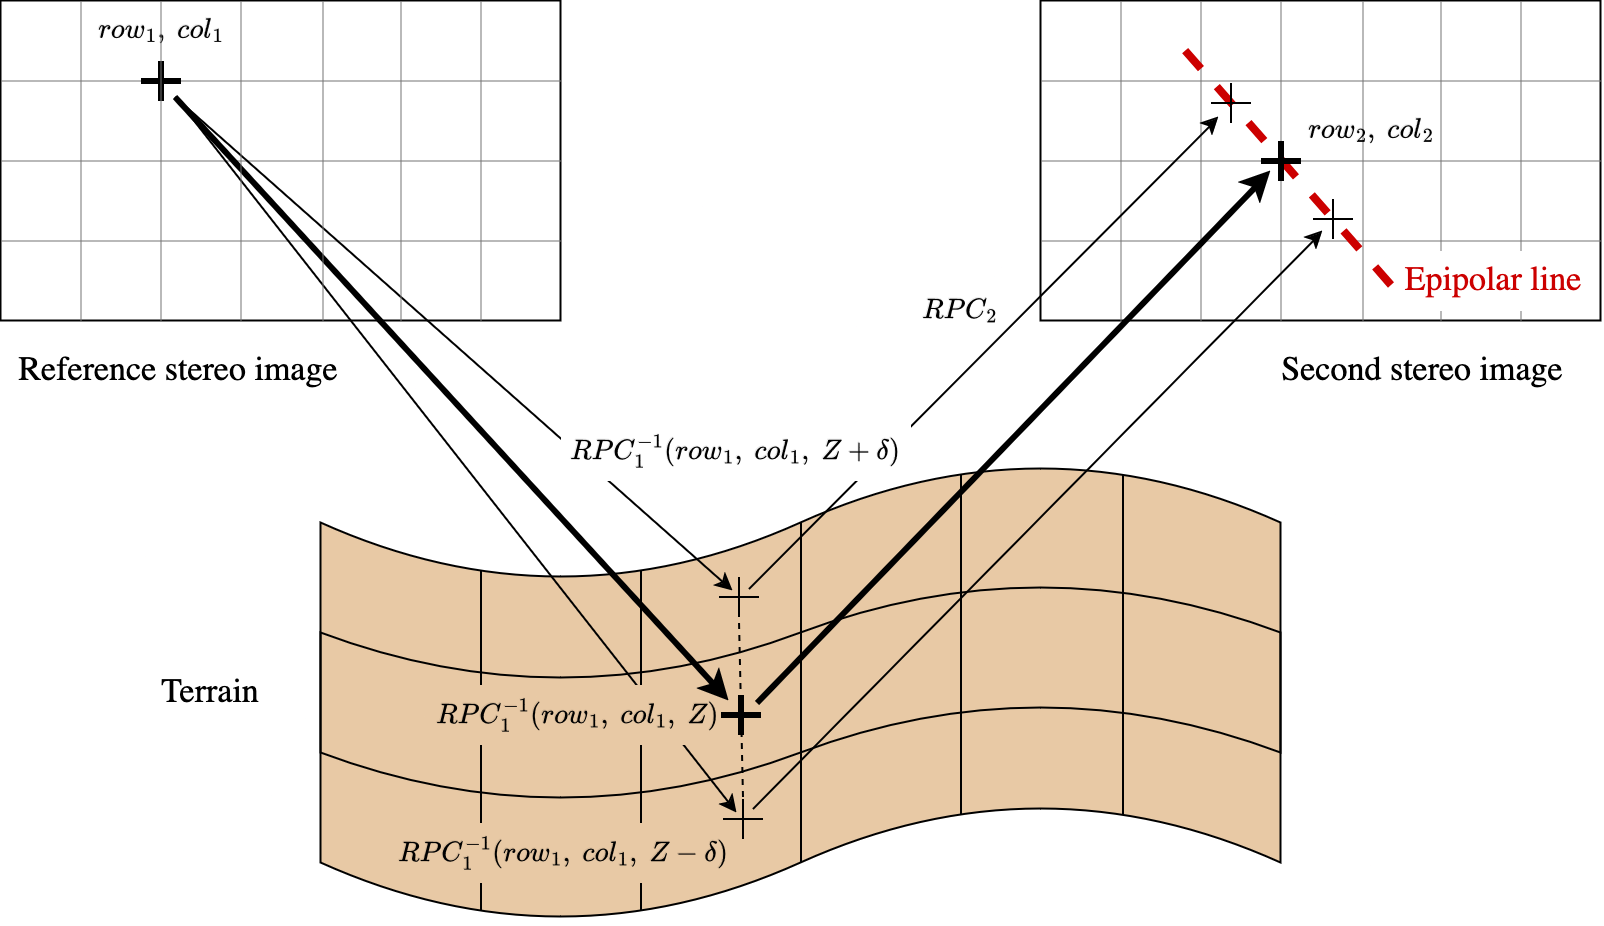
\includegraphics[width=\linewidth]{Images/Chap_1/epipolar_lines.png}
    \caption{Computation of an epipolar line for a pixel using small height variations}
    \label{fig:epipolar_lines}
\end{figure}

In order to determine the deformation grid, \cref{eq:epipolar_transfer} is evaluated with an elevation $Z_{coarse}$ extracted from the low resolution elevation model, and for small variations of altitude $Z_{coarse}\pm\delta$. Those three points allow to compute the direction of epipolar lines for every pixel of both images as in \Cref{fig:epipolar_lines}. This method generates the deformation grid $g_{e1}$ joining every epipolar coordinate $(row_e, ~col_e)$ to its position in the reference image $(row_1, ~col_1)$:
\begin{align}\label{eq:epipolar_grid}
    g_{e1}(row_e, ~col_e) = (row_1, ~col_1)
\end{align}

A similar grid $g_{e2}$ is determined for the secondary image, which is computed jointly with $g_{e1}$. For more details on the way epipolar grids are computed, we refer to \cite{michel_new_2020}. Using those grids, it is possible to resample the reference and secondary images in their respective epipolar geometry. 

\begin{remark}
    With this method, an object whose elevation equals that of the reference elevation model $Z_{coarse}$ (\ie the geoid, or a low resolution \acrshort{dsm} such as the Copernicus \acrshort{dem}) has a disparity of $0$ between epipolar images. After the dense matching step, a disparity of $0$ would mean that the object has the same altitude than that of the low resolution elevation model.
\end{remark}

Because the geolocation models have a limited precision, there might be a misalignment left in the epipolar grids. To correct this error, a set of \acrfull{sift} points \cite{lowe_distinctive_2004} is computed between the reference and secondary epipolar images. For every match, the difference between their rows is computed. The secondary epipolar grid is then corrected so that row differences are null on average. Once aligned epipolar grids have been obtained, stereo images can been resampled in a epipolar geometry which minimizes the errors between \acrshort{sift} points.

Along side epipolar grids can be computed the disparity to altitude ratio $r_{alt}$, which corresponds to the altimetric shift resulting from a shift of 1 in disparity. In other words, if a pixel has a disparity of $0$, then its altitude will be $Z_{coarse}$, and if it has a disparity of $1$, then its altitude will be $Z_{coarse}+r_{alt}$. $r_{alt}$ is also called the altimetric ratio, and provides an estimation of the altimetric resolution of the final \acrshort{dsm}. The altimetric ratio varies along an image, but its variations are small enough so that we can safely approximate it by a constant. We will make extensive use of the altimetric ratio $r_{alt}$ in \Cref{chap:elevation_intervals} to compare the uncertainty of \acrshort{dsm} with different altimetric resolutions.

Once the input images in sensor geometry have been resampled into epipolar geometry, the disparity of every pixel can be computed using dense matching algorithms.

\subsection{Stereo Matching}\label{sec:stereo_matching}
Dense matching refers to the pairing of every pixel between two images. It differs from sparse matching were only a restricted sets of pixels must be matched in both images. Sparse matching is used for registering the different channels of an image if they have been acquired separately, for instance using push-broom sensors. For constructing high-resolution \acrshort{dsm}, dense matching is necessary as we are interested in estimating the disparity at a pixel scale.

Dense matching can be performed once epipolar images have been computed. As stereo matching is an important problem in computer vision, multiple algorithms have been proposed to compute a dense disparity map $\mathcal{D}$ mapping erach pixel $(\rowcol)$ to its disparity $d$. Dense matching algorithms can be broadly classified into two categories: classical approaches following the steps outlined by Scharstein \etal \cite{scharstein_taxonomy_2001}, and deep-learning based methods \cite{laga_survey_2022}.
\begin{remark}
	In the domain of stereo matching, the reference image is often referred to as the \textit{left} image, and the secondary image is the \textit{right} image.
\end{remark}

Recently, deep-learning methods have greatly improved the results of stereo matching algorithms for both remote sensing applications \cite{chebbi_deepsim-nets_2023} and more general applications \cite{tosi_survey_2024} such as robotics, autonomous cars or augmented reality. Best results on famous benchmarks have been obtained using 2D an 3D convolution neural networks end-to-end deep-learning approaches \cite{guo_openstereo_2024, liu_playing_2024}. Those models usually undergo a supervised training, with many datasets being available for stereo processing, especially for autonomous cars \cite{geiger_are_2012, geiger_vision_2013}.

There are less open satellite datasets due to the costs and copyrights of satellite images, even if more datasets tends to be released \cite{bosch_semantic_2018, le_saux_data_2019, huang_urban_2022}. Obtaining ground truth data for satellite imagery is also challenging: as classical approaches such as structured light for producing ground truth disparity cannot be used. Instead, costly airborne campaigns are carried-out, and the acquired elevation data must be converted into disparity maps, which is a complex process \cite{cournet_ground_2020}. Additionally, large models often face generalization challenges, particularly when applied to images that differ from their training datasets. It is especially true in the case of satellite imagery \cite{mari_disparity_2022, jiang_rethinking_2024}, as there is a large variety of landscapes, sensors and acquisitions angles to consider. Furthermore, the radiometry can change depending on the time of the day where the acquisition occurred, and landscapes change can also vary greatly between two seasons. All those factors make the training of a performing and generalizable network for satellite imagery quite challenging. Non-supervised algorithm could avoid some of those drawbacks, but they do not present the same performances as supervised networks.

Even though deep stereo algorithms produces exciting results, we will not focus on deep end-to-end algorithms in this thesis and instead restrict ourselves to so-called \textit{classical} methods used in satellite stereo pipelines. Those methods have the advantage of relying on an extensive literature on the subject. More importantly, those methods are explainable as they do not have a ``black-box'' structure similar to that of end-to-end networks. Their interpretability is crucial when modelling and propagating their uncertainty, which is particularly relevant in the context of this thesis.

Classical approaches usually encompass the following steps\cite{scharstein_taxonomy_2001}:
\begin{itemize}
    \item matching cost computation
    \item cost aggregation
    \item disparity optimization and computation
    \item disparity refinement
\end{itemize}
\Cref{fig:stereo_matching_pipeline} illustrates those different steps. We will detail each step into more details in the following sections. We consider the case of the Pandora correlator developed at \acrshort{cnes} (\url{https://github.com/CNES/Pandora}), which is used by the \acrshort{cars} pipeline for the dense matching step.

\begin{figure}
	\centering
	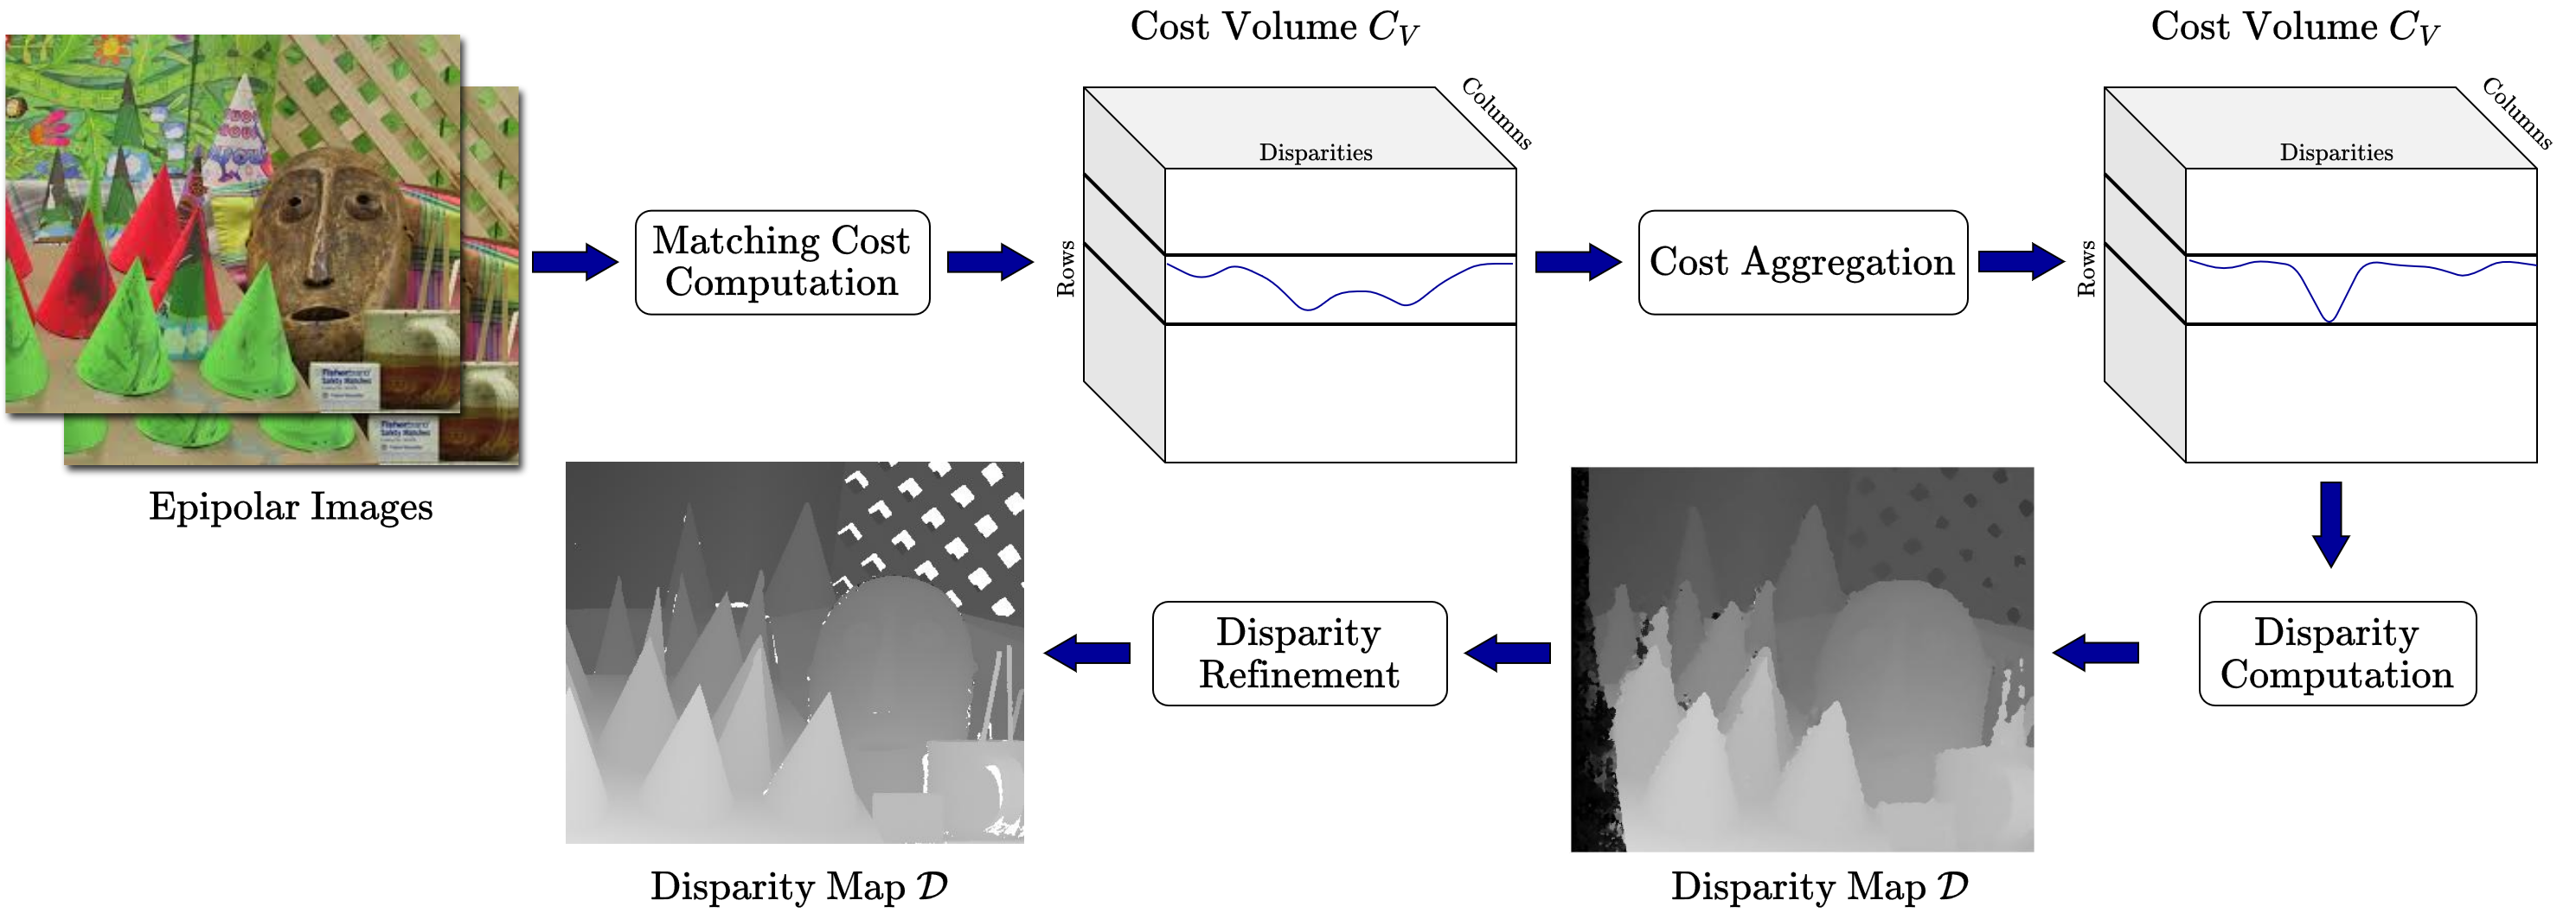
\includegraphics[width=\linewidth]{Images/Chap_1/stereo-matching_pipeline.png}
	\caption{The different steps of classical dense stereo matching algorithms.}
	\label{fig:stereo_matching_pipeline}
\end{figure}

\subsubsection{Matching Cost Computation}\label{sec:cost_volume_computation}
To determine pairs of matching pixels, we first start by measuring the cost of matching two pixels together. Pixels with similar values and similar surroundings will have a low matching cost, while dissimilar pixels will have a high matching cost. Each matching cost value is evaluated using a cost function, which is a mapping $f$ from subsets of the left and right images to $\mathbb{R}$. A cost function $f$ measures the dissimilarity between the two subsets of the left and right images.. \Cref{ex:cost_functions} provides different instances of cost functions.

\begin{example}\label{ex:cost_functions}
	Simple instances of cost functions include the Sum of Absolute Differences (SAD), the Zero Normalized Crossed Correlation (ZNCC)  \cite{hannah_computer_1994}, the CENSUS transform \cite{zabih_non-parametric_1994} and MC-CNN \cite{zbontar_stereo_2016}, which will be detailed in the following paragraphs.
	
	Given two windows $W_L$ and $W_R$ from the left and right images, the SAD cost function is defined as follows:
	\begin{equation}
		f_{SAD}(W_L, W_R)  = \sum_i\sum_j | W_L(i,j) - W_R(i,j) |
	\end{equation}
	Low $f_{SAD}$ values indicate that the windows are similar, while high values indicate noticeable differences. A $f_{SAD}$ value of $0$ indicates that the windows are identical. This cost function is probably the simplest cost function one could imagine, and will be used in \Cref{chap:propagating} to didactically illustrate how uncertainty models can be propagated throughout a cost function. However, this cost function is not usually employed in practice as it is based on intensity differences, and is thus very sensitive to radiometric changes. It can however be a fast and easy way to have a first estimate of similarities between multiple patches. The SAD can also be used for motion estimation and image/video compression \cite{richardson_h264_2006}.
	
	The ZNCC cost function is defined as the correlation coefficient between both images:
	\begin{equation}
		f_{ZNCC}(W_L, W_R)  = \sum_i\sum_j \frac{(W_L(i,j)  - \tilde{W}_L) (W_R(i,j)  - \tilde{W}_R) }{\sigma_L\sigma_R}
	\end{equation}
	where $\tilde{W}$ refers to the mean value of a window, and $\sigma$ its standard deviation. Negatively correlated windows would present a ZNCC value of $-1$ and positively correlated windows present a ZNCC value of $1$. Contrary to the SAD cost function, matching windows will be indicated by a high value of the ZNCC. It is thus not \textit{strictly} a cost function but rather a similarity function. It is not a problem, as multiplying $f_{ZNCC}$ by $-1$ will transform it into a cost function. Another formulation could be to say that the $ZNCC$ is a \textit{maxitive} cost function, in the sense where potential matches are found by searching for its maximum. Conversely, the SAD is a \textit{minitive} cost function in the sense where potential matches are indicated by a minimal cost. The $ZNCC$ cost function performs well in homogeneous areas when computed over a large windows. However in an urban settings, it struggles to correctly estimate buildings boundaries.
	
	The CENSUS cost function needs to be a bit more detailed. For a squared window $W$ with a side of $2n+1$ pixels, we first compare the value of each pixel of the window with the center pixel. This gives a binary string where $1$ indicates that the value of the pixel is superior to that of the center pixel. For instance if we consider the two $3\times3$ following windows $W_L, W_R$:
	$$
    \begin{bmatrix}
        155 & 133 & 97 \\
        80 & 110 & 132 \\
        100 & 102 & 120
    \end{bmatrix}
    \qquad
    \begin{bmatrix}
        175 & 153 & 133 \\
        100 & 130 & 152 \\
        120 & 135 & 125
    \end{bmatrix}
	$$
	Then comparing each of their pixel to the center of the windows will yield the following binary strings (expressed here as matrices):
	$$
    \begin{bmatrix}
        1 & 1 & 0 \\
        0 &  & 1 \\
        0 & 0 & 1
    \end{bmatrix}
    \qquad
    \begin{bmatrix}
        1 & 1 & 1 \\
        0 &  & 1 \\
        0 & 1 & 0
    \end{bmatrix}
	$$
	The cost function $f_{CENSUS}$ is finally obtained by taking the Hamming distance (\ie the number of different bits between those two strings):
	\begin{equation*}
		f_{CENSUS}(W_L, W_R) = 3
	\end{equation*}
	
	The CENSUS cost function compares relative intensity variations, it is thus less sensitive to variations of intensities between images, such as a change of exposure for instance. Similarly to the SAD, two similar patches will tend to have a low value.
	
	The MC-CNN cost function \cite{zbontar_stereo_2016} is using a convolutional neural network architecture to measure the similarity between patches. It was train on $11\times 11$ patches from stereo images from the Kitti \cite{geiger_vision_2013, menze_object_2015} and Middlebury \cite{scharstein_taxonomy_2001,scharstein_high-accuracy_2003,hirschmuller_evaluation_2007,scharstein_learning_2007,scharstein_high-resolution_2014} datasets. They first trained a siamese neural network to compute a vector of features for each patch, then compute the dot product between both vectors to obtain a similarity measure. MC-CNN is thus a maxitive cost function. \Cref{fig:mccnn} details the architecture of the network. Although it has been trained on stereo images of autonomous cars (Kitti) and stereo images of toys (Middlebury), it generalizes well to satellite images \cite{defonte_evaluation_2021}.
	
	{\centering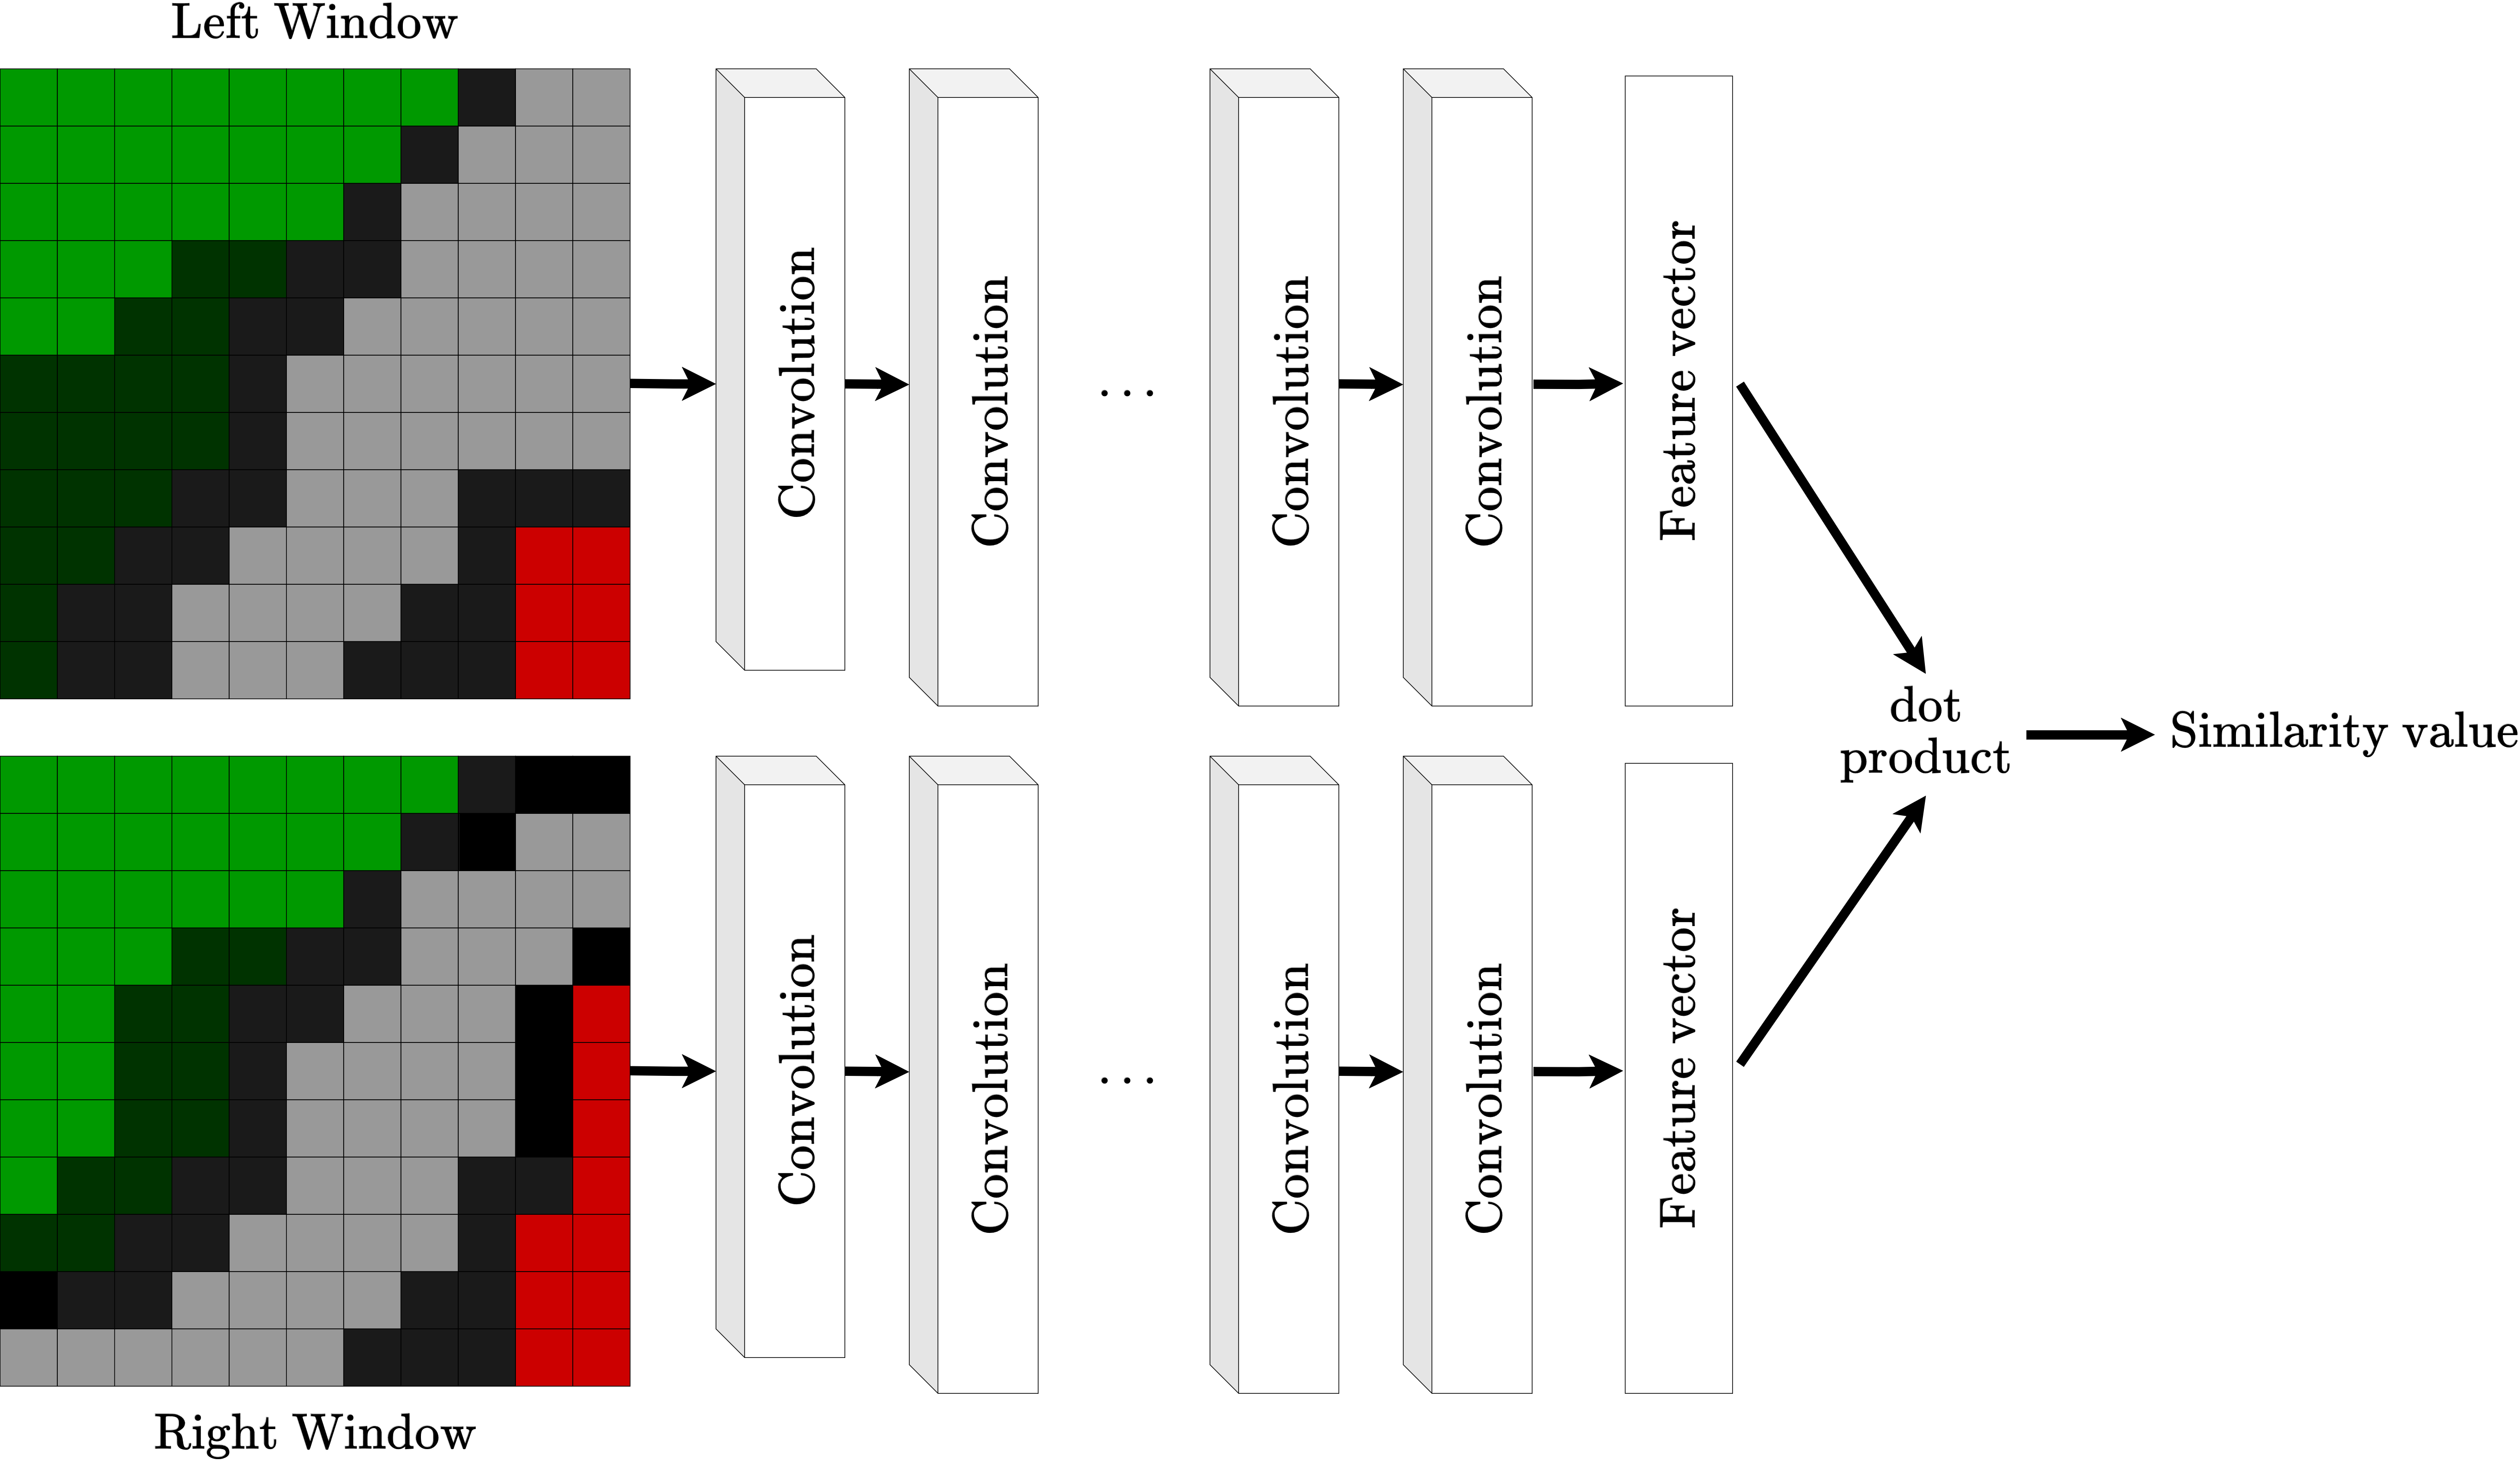
\includegraphics[width=0.8\linewidth]{Images/Chap_1/MCCNN.png}\captionof{figure}{MC-CNN architecture}\label{fig:mccnn}}
\end{example}

Matching costs are evaluated for every potential pairs of pixels whose corresponding disparity lies in a given disparity range. Matching cost values are stored in an array of data, called \textit{cost volume} (\Cref{fig:cost_volume}). The term volume is used as a matching cost value is determined by three coordinates in the cost volume: the row and column $(\rowcol)$ of the left pixel as well as the considered disparity $d$:
\begin{equation}\label{eq:cost_volume}
    C_V(\rowcol, ~d) = f(W_L(\rowcol),  W_R(\rowcol+d))
\end{equation}
where $W_L(\rowcol)$ is a window centered on the pixel at coordinates $(\rowcol)$ in the left image, and $W_R(\rowcol+d)$ is a window centered on the pixel at $(\rowcol+d)$ in the right image. Some padding is usually added to the images to avoid problems near borders where the column $col+d$ would not be defined. Given a pixel in the left image $(\rowcol)$, matching cost values for every considered disparity form what is called a cost curve. In theory, the correct disparity for a match is determined by finding the minimum of the cost curve (for minitive cost functions such as SAD or CENSUS). \Cref{fig:cost_volume} represents a cost volume, and one of its cost curves where potential matches have been highlighted. In the rest of this thesis, we will consider that a cost function is always minitive unless specified otherwise. In practice, directly estimating the disparities from the cost volume is not efficient as we only consider local information. The resulting disparity map is often very noisy, as can be seen in \Cref{fig:disparity_map_no_sgm}. In order to reduce this noise, one solution is to aggregate the costs of neighboring pixels in the cost volume.

\begin{figure}
	\centering
	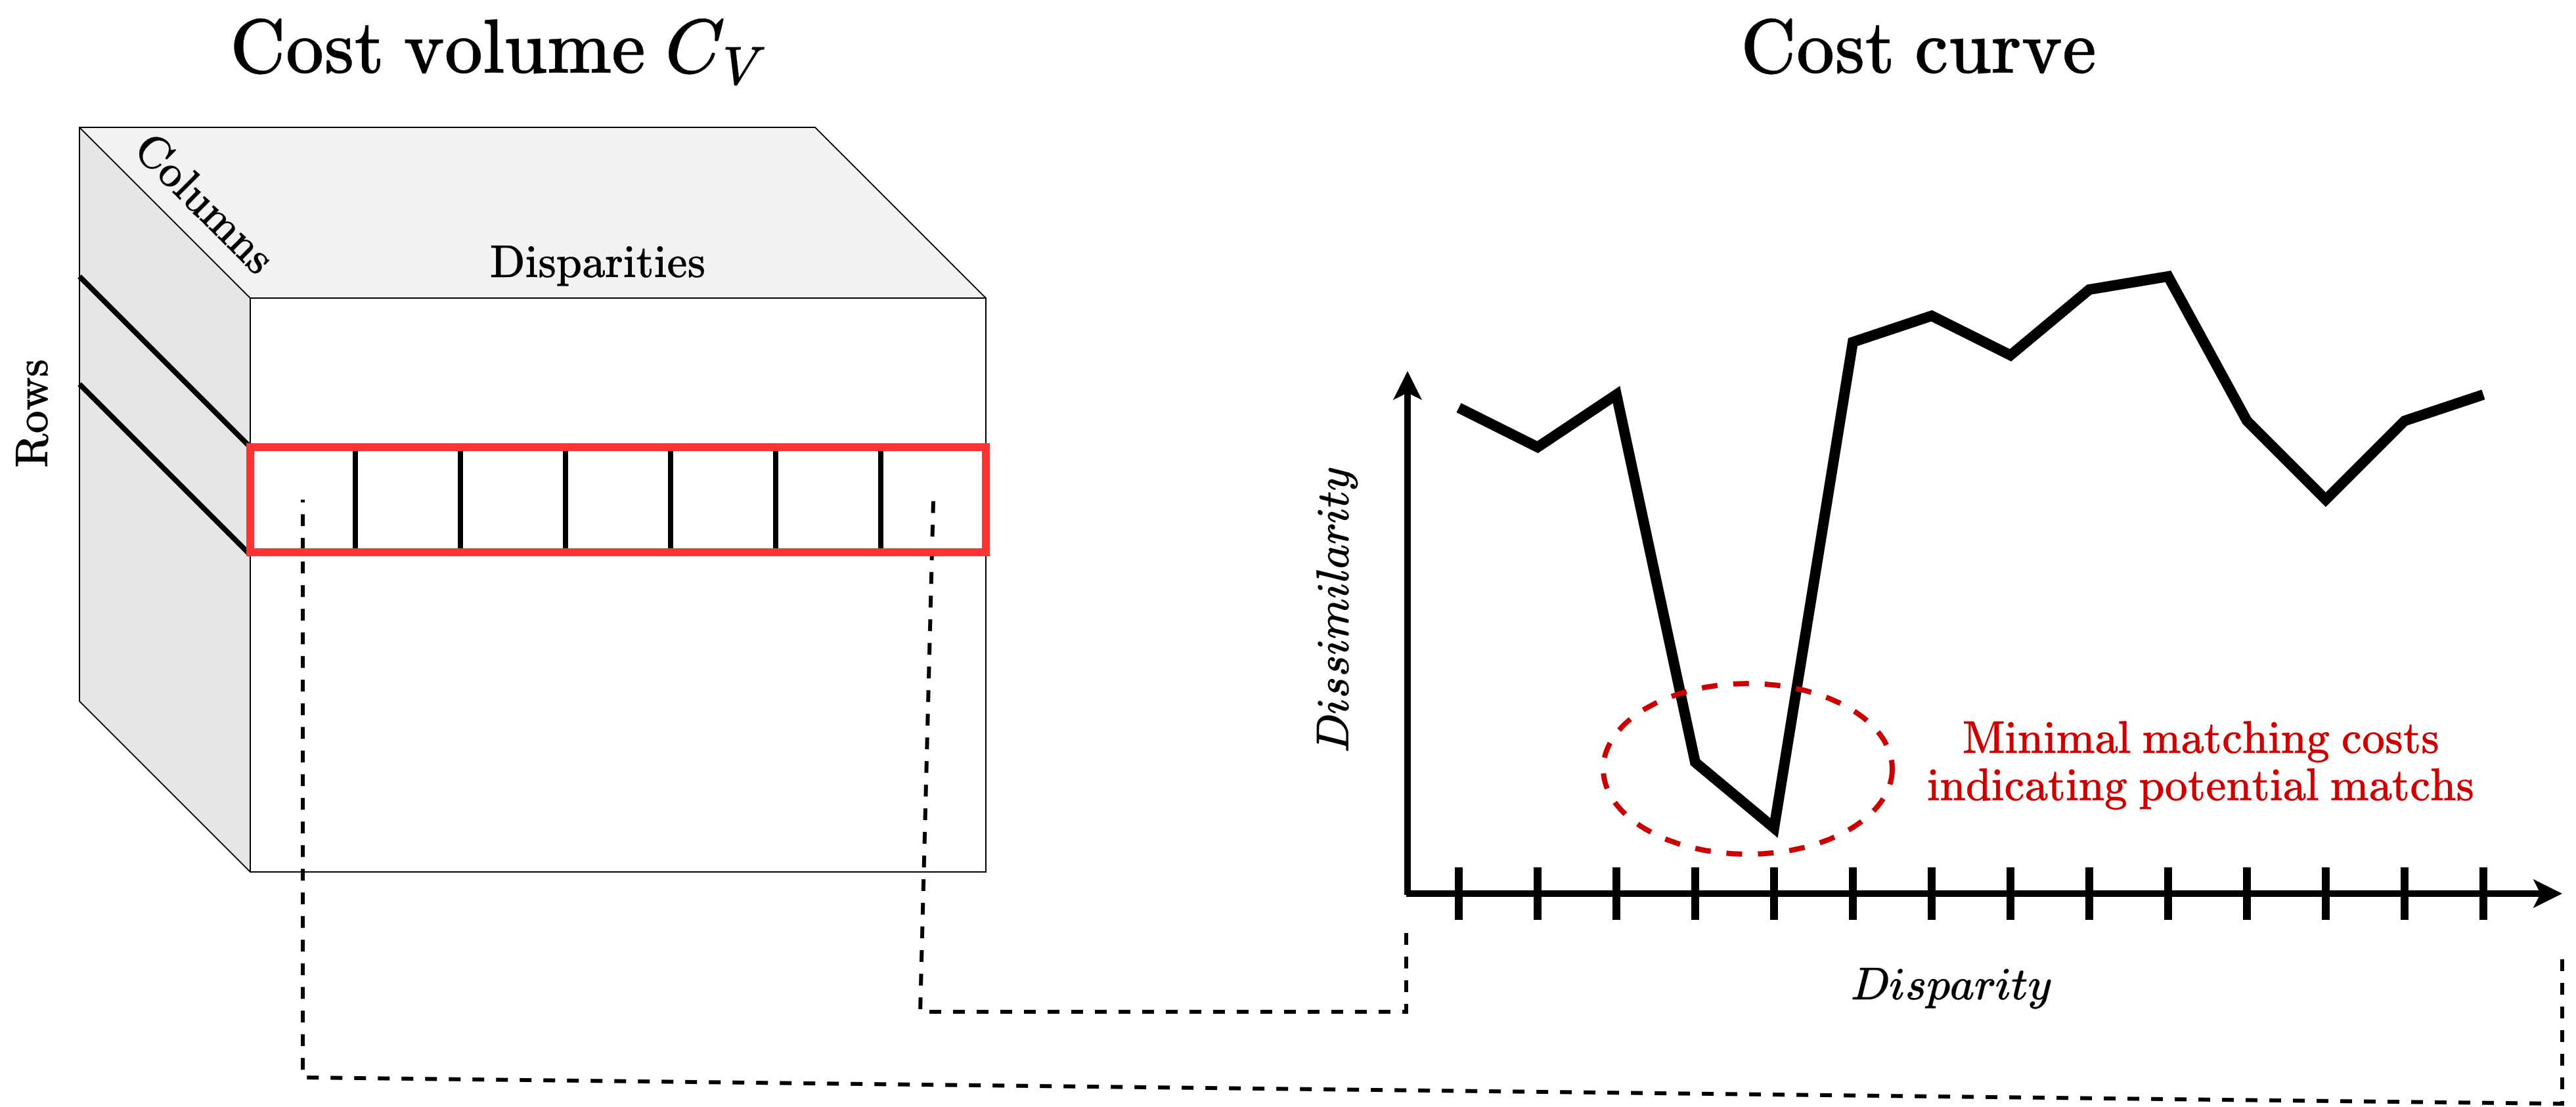
\includegraphics[width=\linewidth]{Images/Chap_1/Cost_volume.png}
	\caption{Matching cost volume and one of its cost curve}
	\label{fig:cost_volume}
\end{figure}

\begin{figure}
    \begin{subfigure}[t]{0.42\linewidth}
        \flushleft
        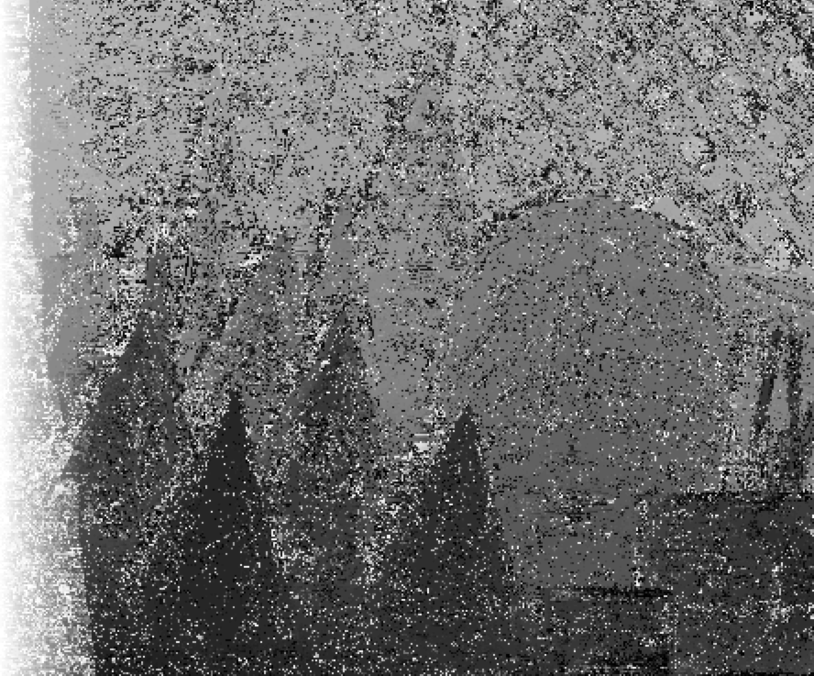
\includegraphics[width=\linewidth]{Images/Chap_1/disparity_map_no_sgm.png}
        \caption{Disparity with local cost only}
        \label{fig:disparity_map_no_sgm}
    \end{subfigure}\hfill
    \begin{subfigure}[t]{0.514\linewidth}
        \flushright
        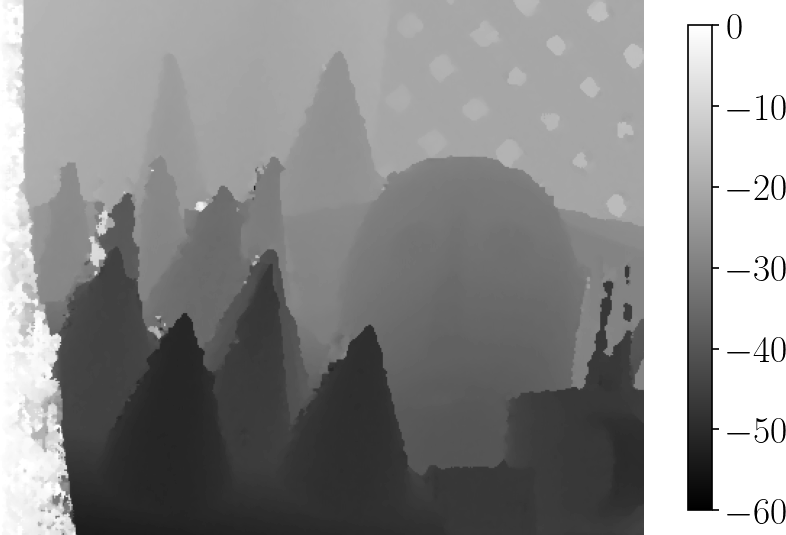
\includegraphics[width=\linewidth]{Images/Chap_1/disparity_with_sgm.png}
        \caption{Disparity with \acrshort{sgm} regularization}
        \label{fig:disparity_map_with_sgm}
    \end{subfigure}
    \caption{Disparity map without and with \acrshort{sgm} regularization.}
    \label{fig:disparity_map_with_and_without_sgm}
\end{figure}

\subsubsection{Cost Aggregation}
The usage of windows in the calculation of the cost function allows to take into consideration the surrounding of pixels to better measure their similarity. However, window based approaches, which are mostly square-shaped, also present the disadvantage of struggling to correctly identify matches near object borders \cite{hirschmuller_real-time_2002}. This is usually called an adherence effect, represented in \Cref{fig:adherence_window}. In \Cref{fig:adherence_left}, we can see that the considered pixel is at the border of an object with the left window $W_L$ spanning over both part of the border. In \Cref{fig:adherence_cost_curve}, we can see that the minimum of the cost curve (around disparity -40) is not exactly located at the true disparity. This is in part due to the fact that $W_L$ contains pixels from two objects with different disparities, which influences the matching cost values. A low matching cost thus does not necessarily mean that the center pixels constitute a match. The term ``adherence'' is used as the matching windows tend to falsely estimate the shift in disparity near objects border, as if it adhered to the object. Other work have been proposing to use a spatial weighting \cite{kuk-jin_yoon_locally_2005}, segmentation \cite{hutchison_segmentation-based_2007}, windows with different shapes \cite{ke_zhang_cross-based_2009, buades_reliable_2015} to solve this problem. 

\begin{figure}
    \begin{subfigure}[t]{0.35\linewidth}
        \flushleft
        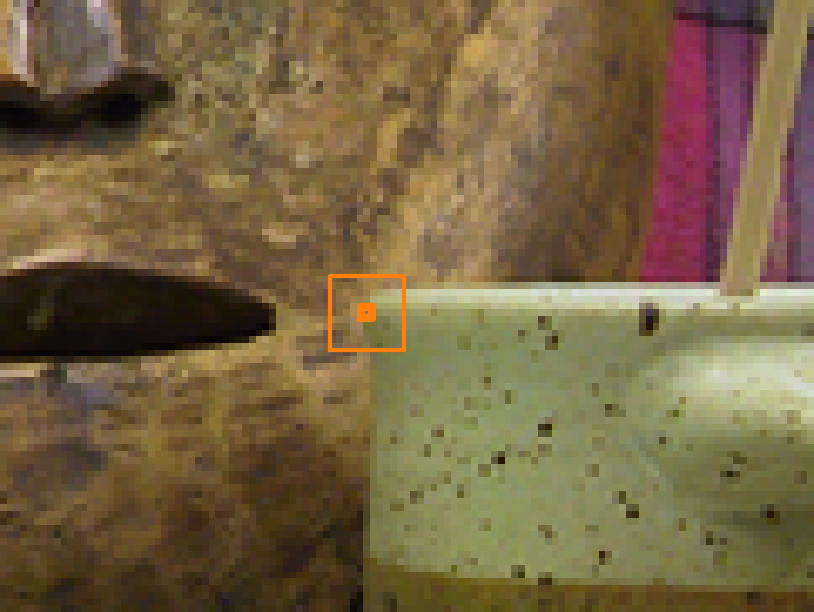
\includegraphics[width=\linewidth]{Images/Chap_1/adherence_overview_left.png}
        \caption{Left image with $W_L$ in orange}
        \label{fig:adherence_overview_left}
    \end{subfigure}\hfill
    \begin{subfigure}[t]{0.6\linewidth}
        \flushright
        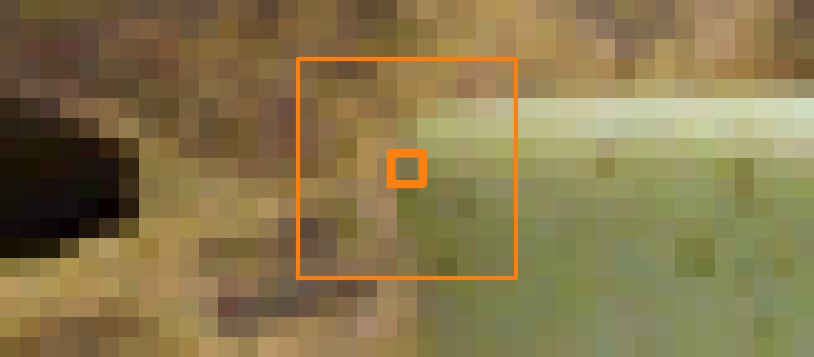
\includegraphics[width=\linewidth]{Images/Chap_1/adherence_left.png}
        \caption{Zoom over $W_L$, in orange}
        \label{fig:adherence_left}
    \end{subfigure}\\
    \begin{subfigure}[t]{\linewidth}
        \flushright
        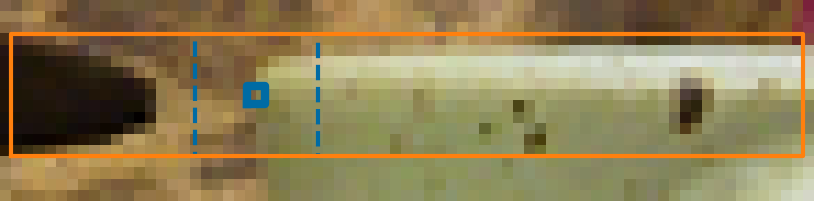
\includegraphics[width=0.87\linewidth]{Images/Chap_1/adherence_right.png}
        \caption{Right image. Considered windows in orange, and $W_R$ for the true disparity in blue}
        \label{fig:adherence_right}
    \end{subfigure}\\
    
    \begin{subfigure}[t]{\linewidth}
        \centering
        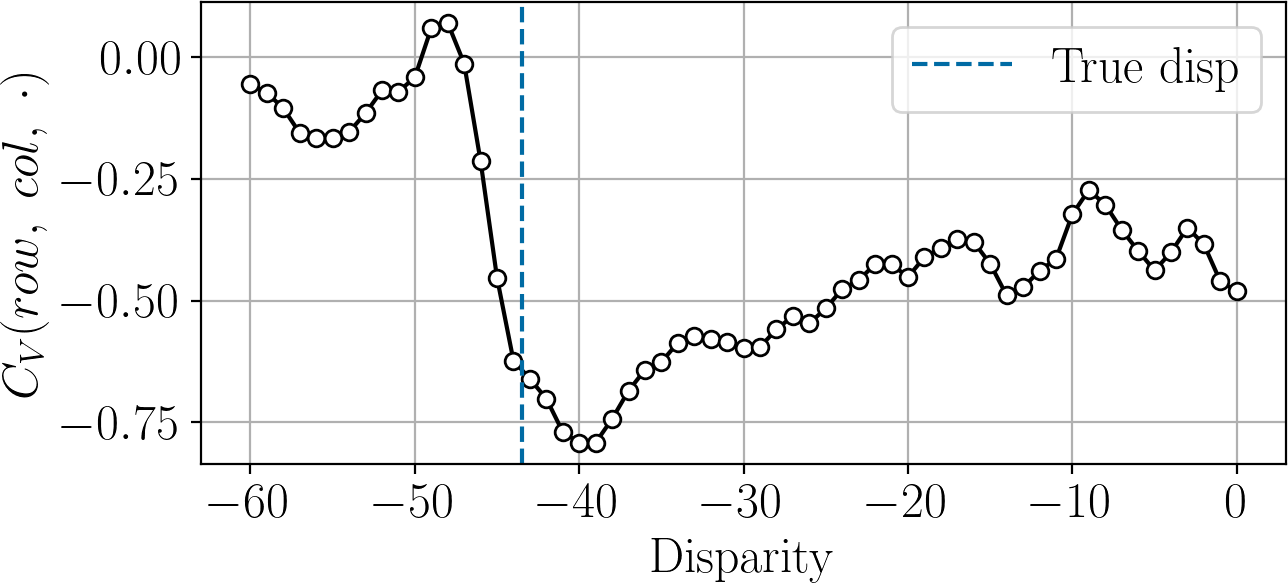
\includegraphics[width=\linewidth]{Images/Chap_1/adherence_cost_curve.png}
        \caption{Corresponding minitive cost curve ``$-f_{ZNCC}$''}
        \label{fig:adherence_cost_curve}
    \end{subfigure}
    \caption{Example of the adherence effect. \Cref{fig:adherence_overview_left,fig:adherence_left} present the left window $W_L$ at the border of an object. \Cref{fig:adherence_right} presents all the windows from the right image in the considered disparity range, that will be compared to $W_L$. The window corresponding to the true disparity appears in blue. \Cref{fig:adherence_cost_curve} details the corresponding cost curve, where the true disparity does not correspond to the minimum of the cost curve.}
    \label{fig:adherence_window}
\end{figure}

After computing the matching cost, information from neighboring pixels can be incorporated in the cost volume. A first approach is to aggregate different parts of the cost volume. Usually, costs of pixels belonging to the same objects are aggregated using different methods for segmentation \cite{ke_zhang_cross-based_2009, ji_superpixel_2021}. This part is not always present in algorithms, as we will see we can consider global information directly when determining the disparity map.

\subsubsection{Disparity Optimization and Computation}
Computing the disparity map from the cost volume can be done in several ways. So-called local methods apply a direct \textit{winner-takes-all} strategy, where the $\argmin$ of every cost curve is kept as the selected disparity. On the other hand, global method use the information contained in the cost volume to solve an optimization problem, where the objective is to compute the disparity map $\mathcal{D}$ minimizing an energy function expressed as follows:
\begin{equation}
    E(\mathcal{D}) = E_{data}(\mathcal{D}) + \lambda E_{smooth}(\mathcal{D})
\end{equation}
where $\lambda$ is a scalar for tuning the importance of the regularization term $E_{smooth}$. Usually, the data term is directly computed from the cost volume as:
\begin{equation}\label{eq:global_methods}
    E_{data}(\mathcal{D}) = \sum_{row,~col}C_V(\rowcol,~\mathcal{D}(\rowcol))
\end{equation}
The regularization term $E_{smooth}$ can take numerous forms, usually measuring if the neighboring disparities possess similar values \cite{scharstein_taxonomy_2001}. Then a local minimum for this energy is found using various methods, such as Markov Random Fields \cite{boykov_markov_1998, sun_stereo_2003}, graph cuts \cite{kolmogorov_computing_2001} or minimum spanning trees \cite{zureiki_stereo_2008, qingxiong_yang_non-local_2012}. Those algorithms improves performances in comparison to local methods, but can be computationally expensive.

A most popular method is called \acrfull{sgm} \cite{hirschmuller_accurate_2005}: it aims at incorporating regularization constraints to the cost volume similarly to global methods, while being processed with relative low computational cost like local methods. Its name It is, in a way, in-between local and global methods. This is the method used in the \acrshort{cars} pipeline, and for experiments in this thesis. In a few words, for each pixel, the \acrshort{sgm} algorithm computes a regularized cost volume, which is based on the regular cost volume (the $E_{data}$ term), and adds cost penalties to the disparities differing from that of their neighboring pixels (the $E_{smooth}$ term). Although the formulation of the \acrshort{sgm} algorithm can be expressed in a few equations, understanding its inner workings is more complex. We will first present its mathematical formulation in \cref{eq:sgm,eq:sgm_penalties}, and use \Cref{fig:sgm} to illustrate its effect on (a portion of) a cost curve. \Cref{fig:cost_curve_with_without_sgm} presents the effect of \acrshort{sgm} regularization on different cost curves and \Cref{fig:disparity_map_with_and_without_sgm} presents the effect of \acrshort{sgm} regularization on the final disparity map. Formally, for every pixel $p=(\rowcol)$, the cost volume is explored in multiple directions as in \Cref{fig:sgm_directions}.

\begin{figure}
	\centering
	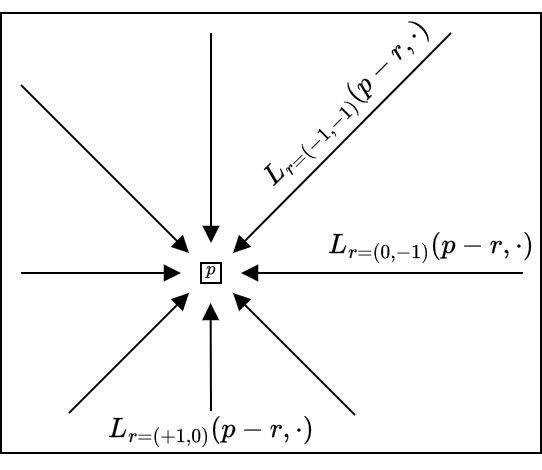
\includegraphics[width=0.5\linewidth]{Images/Chap_1/SGM_directions.png}
	\caption{\acrshort{sgm} regularization with $8$ directions}
	\label{fig:sgm_directions}
\end{figure}

The cost is regularized for each direction $r$ to take into account the best disparity $d$ along that direction. A direction can be for instance $r=(0,~1)$, meaning that we will look at same row and travel to the right of the image when browsing direction $r$. Given two positive scalars $P_1<P_2$, the regularized cost $L_r$ along direction $r$ and at disparity $d$ is expressed with the following recursive formulation:
\begin{align}\label{eq:sgm}
    L_r(p,d) = C_V(p,d) + \min_\delta \left(L_r(p-r,~\delta) + R(d, ~\delta)\right)
\end{align}
where $\delta$ is a dummy variable to explore the disparity range, and where $R(d, ~\delta)$ equals:
\begin{align}
    R(d, ~\delta) = &P_1\cdot\mathds{1}(|d-\delta|=1) + P_2\cdot\mathds{1}(|d-\delta|\geqslant 2) - \min_k L_r(p-r,~k) \label{eq:sgm_penalties}
\end{align}
Here, $\mathds{1}$ is the indicator function. The first term of \cref{eq:sgm} is the cost volume, which can be compared to $E_{data}$ in \cref{eq:global_methods}. The second term is similar to the regularisation term $E_{smooth}$. This term can be seen as the regularized cost $L_r(p-r, ~d)$ from the previous pixel in direction $r$, but shifted of $P_1$ for neighboring disparities $d\pm1$, and of $P_2$ for further disparities. The term $\min_k(L_r(p-r,~k))$ prevents $L_r(p,\cdot)$ to diverge to very high values by ensuring that the minimum of $L_r(p-r,~\delta) - \min_k(L_r(p-r,~k))$ always equals $0$. \Cref{fig:sgm} presents $L_r(p-r,~\delta) + R(d, ~\delta)$ for two different disparities $d$ and $d+1$ in the blue frame. The minimum of each curve $L_r(p-r,~\delta) + R(d, ~\delta)$ (blue arrows in the figure) are then added to the matching cost $C_V(p,d)$ to obtain the final regularized cost $L_r(p,d)$. Note that in \Cref{fig:sgm}, the minimum of $L_r(p-r,~\delta)+R(d+1, ~\delta)$ equals $0$, thus $C_V$ is unchanged for this disparity. This is because $d+1$ is the minimum of $L_r(p-r,~\cdot)$. In a way, the regularized matching cost will be a mixture between $C_V(p,\cdot)$ and $L_r(p-r,~\cdot)$. Indeed, the regularized cost $L_r(p-r,\cdot)$ indicates that disparity $d+1$ seems likely, while disparity $d$ is unlikely. On the other hand, the matching cost $C_V(p,\cdot)$ indicates that both disparities $d$ and $d+1$ are likely. The final regularized cost $L_r(p-r,\cdot)$ takes into account that both $C_V(p,\cdot)$ and $L_r(p-r,\cdot)$ agree that $d+1$ is likely, but that there is a disagreement on $d$, and thus slightly increases the regularized cost $L_r(p,d)$. Disparities that seem unlikely to both $C_V(p,\cdot)$ and $L_r(p-r,\cdot)$ lead to a larger increase of the regularized cost $L_r(p,\cdot)$.

\begin{figure}
    \begin{subfigure}[t]{0.49\linewidth}
        \flushleft
        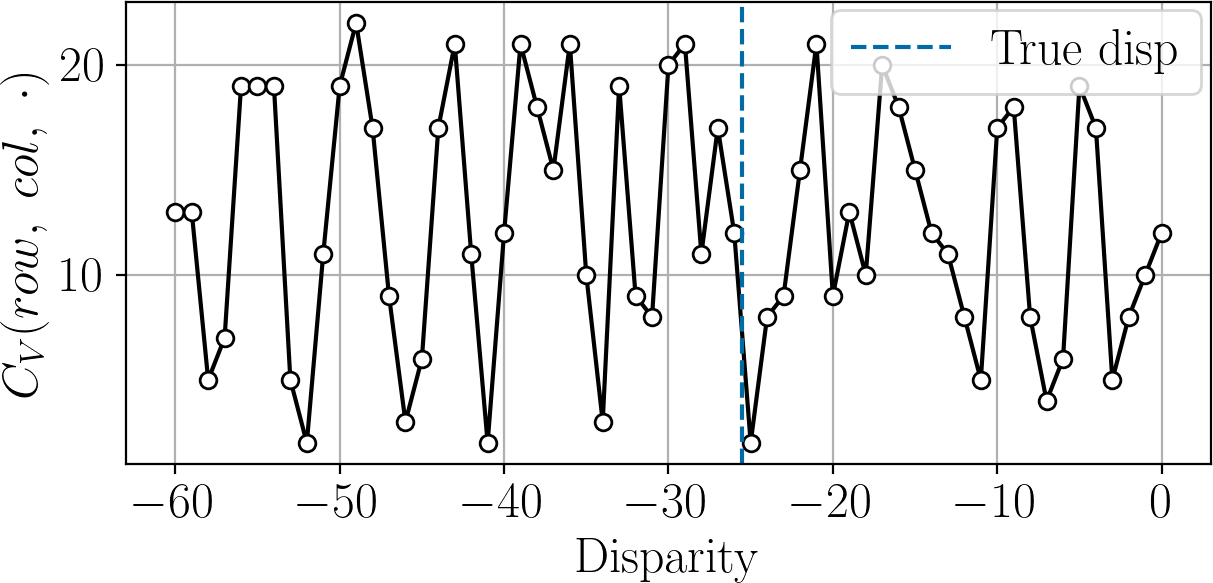
\includegraphics[width=\linewidth]{Images/Chap_1/cost_curve_no_sgm_row_100_col_250.png}
        \caption{Cost curve without \acrshort{sgm}}
        \label{fig:cost_curve_no_sgm_row_100_col_250}
    \end{subfigure}\hfill
    \begin{subfigure}[t]{0.49\linewidth}
        \flushright
        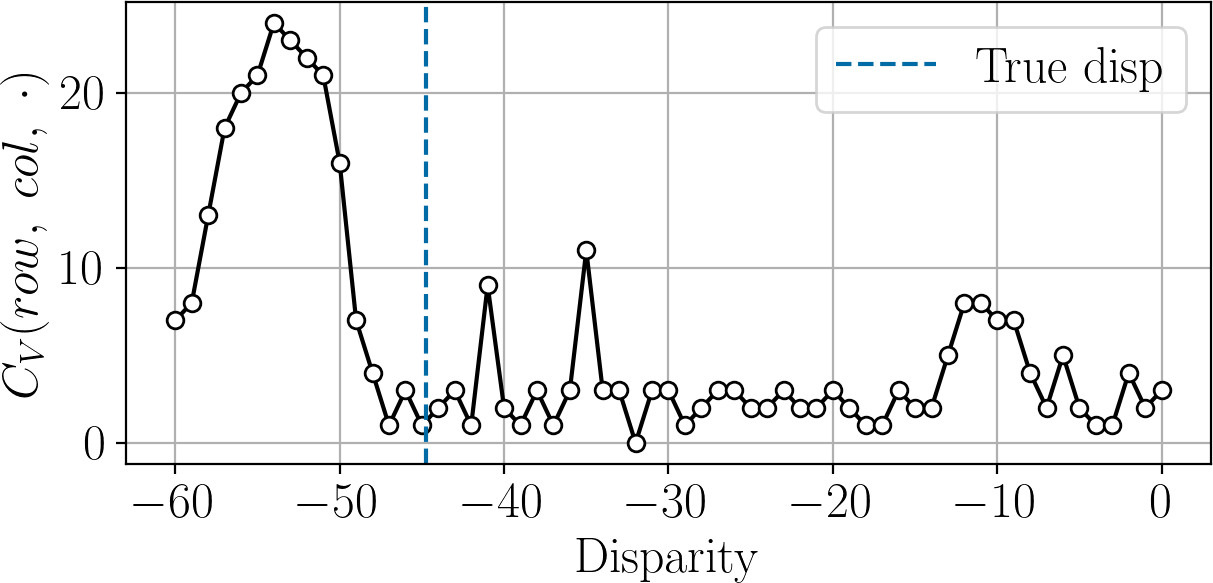
\includegraphics[width=\linewidth]{Images/Chap_1/cost_curve_no_sgm_row_276_col_360.png}
        \caption{Cost curve without \acrshort{sgm}}
        \label{fig:cost_curve_no_sgm_row_276_col_360}
    \end{subfigure}\\
    \begin{subfigure}[t]{0.49\linewidth}
        \flushleft
        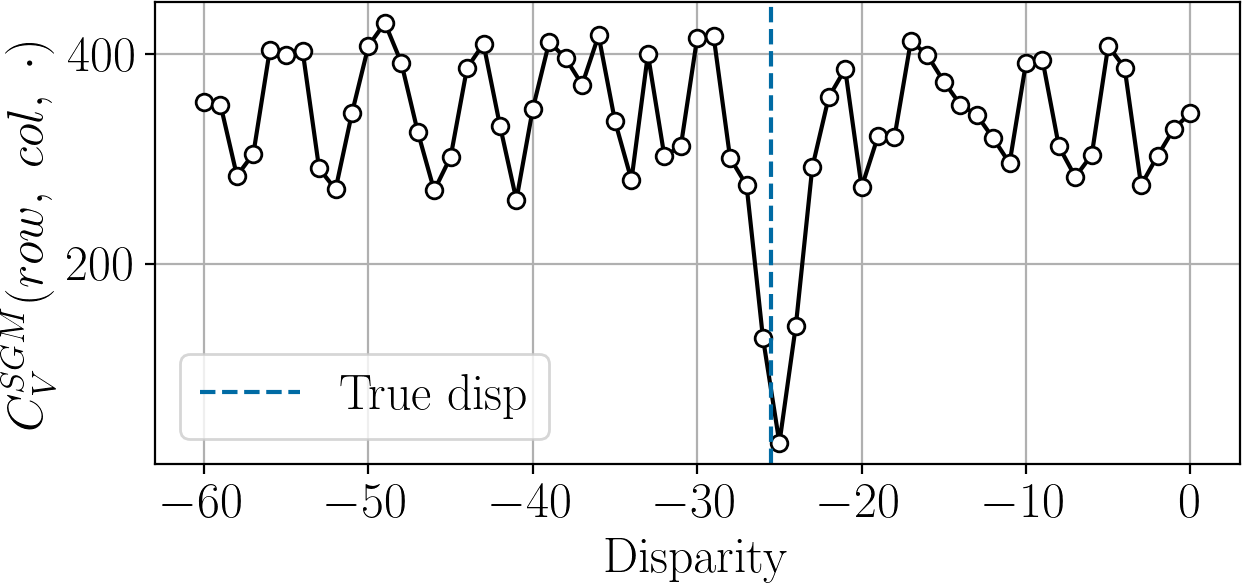
\includegraphics[width=\linewidth]{Images/Chap_1/cost_curve_sgm_row_100_col_250.png}
        \caption{Cost curve from \Cref{fig:cost_curve_no_sgm_row_100_col_250} with \acrshort{sgm}}
        \label{fig:cost_curve_sgm_row_100_col_250}
    \end{subfigure}\hfill
    \begin{subfigure}[t]{0.49\linewidth}
        \flushright
        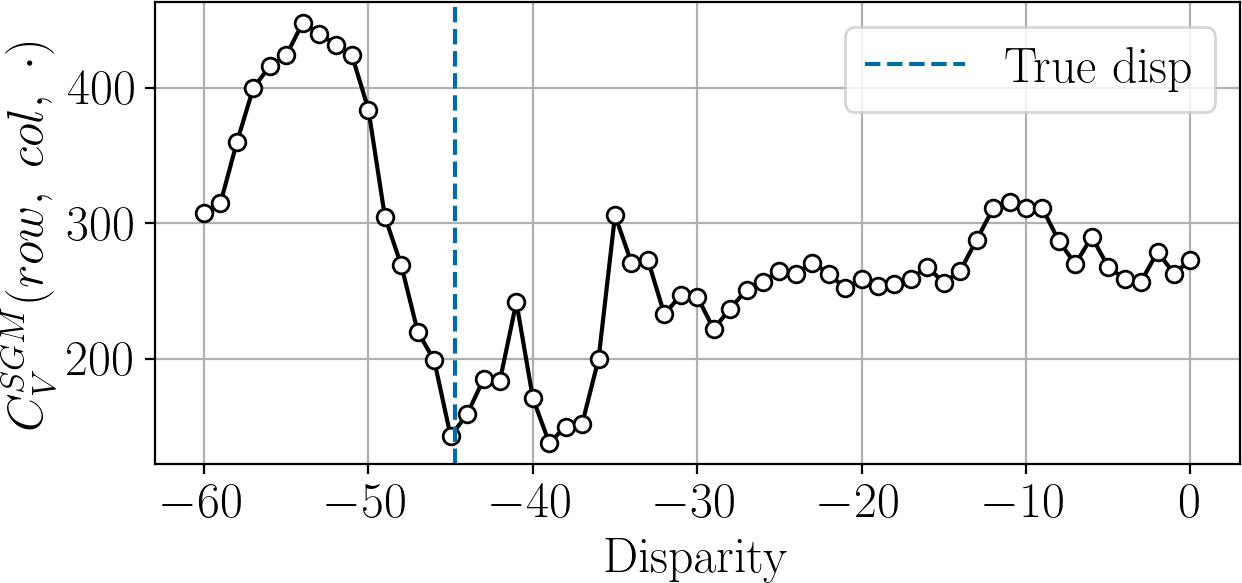
\includegraphics[width=\linewidth]{Images/Chap_1/cost_curve_sgm_row_276_col_360.png}
        \caption{Cost curve from \Cref{fig:cost_curve_no_sgm_row_276_col_360} with \acrshort{sgm}}
        \label{fig:cost_curve_sgm_row_276_col_360}
    \end{subfigure}
    \caption{Different cost curves, with and without \acrshort{sgm} regularization}
    \label{fig:cost_curve_with_without_sgm}
\end{figure}

\begin{remark}
    For the sake of the argument, lets assume that $P_1=P_2$ for now. The value added to $C_V(p, ~d)$ in \eqref{eq:sgm} will be lower than $P_2$ only if $(L_r(p-r,~d) - \min_k L_r(p-r,~k))$ is less than $P_2$. This means that we will always add a penalty of $P_2$ to the cost $C_V$, except if $L_r(p-r,~d)$ is less than $P_2$ away from its minimum. $P_2$ thus represents the penalty that must be overcame in $L_r(p-r,~d)$ in order to not penalize $C_V(p,d)$, or slightly penalize $C_V(p,d)$.
    
    If $P_1<P_2$, then we can draw similar conclusions, except that we also accept to reduce the penalty to $C_V(p,d)$ if a neighboring disparity, \ie $d\pm1$ is less than $P_1$ away from the minimum.
\end{remark}

Formulation of \cref{eq:sgm} is recursive, and thus must be initialized. The regularization curves thus begin at the borders of the image and their value is, by convention, $0$ when undefined. For instance with $r=(0,1)$:
\begin{align*}
    L_r((row, 0),d) = C_V(row, 0 ,d)
\end{align*} 

\begin{figure}
	\centering
	\includegraphics[width=\linewidth]{Images/Chap_1/SGM.png}
	\caption{Schematic explanation of the \acrshort{sgm} algorithm in a single direction $r$. Top: regularized cost $L_r$ at $p-r$. In the blue frame $L_r(p-r,~\delta)+R(d,~\delta)$ for two consecutive disparities $d$ and $d+1$ ($L_r-\min_k L_r$ appears in dotted line for clarity). Penalty $P_1$ appears in yellow, penalty $P_2$ appears in red, the minimum of each curve is denoted by a blue arrow. Bottom left: cost volume $C_V$ at $p$. Bottom right: regularized cost $L_r$ at $p$ where the minima of \textit{all} $L_r(p-r,~\delta)+R(d,~\delta)$ have been added}
	\label{fig:sgm}
\end{figure}

When all regularized cost curves $L_r$ have been computed, they are summed to obtain the regularized cost volume $C_V^{SGM}$:
\begin{equation}
    C_V^{SGM}(p, d) = \sum_r L_r(p,d)
\end{equation}
The cost volume $C^{SGM}_V$ contains the regularized cost for every  considered direction. The number of direction used in our experiments is 8 as in \Cref{fig:sgm_directions}, but more directions can be considered in order to consider a more global coverage. Since the original paper \cite{hirschmuller_accurate_2005}, different variations of the \acrshort{sgm} algorithm have been proposed. For instance using different regularization paths \cite{facciolo_mgm_2015} or a different strategy for the aggregation of costs \cite{poggi_learning_2016}.

In order to insure smooth surfaces, \acrshort{sgm} penalties $P_1$ and $P_2$ must be high enough. This however leads to a reluctance to detect discontinuities in the disparity map. Indeed, \acrshort{sgm} penalizes disparity changes, therefore strong variations of disparity are badly reconstructed. For instance near the border of a building, the term $E_{smooth}$ tends to be predominant, leading to rounded borders and soft edges of buildings, instead of the expected sharp disparity variations. This is even reinforced with the window adherence problem presented in \ref{fig:adherence_window}. \Cref{fig:DSM_toulouse} presents a comparison of two \acrshort{dsm}: one obtained directly from \acrshort{lidar} HD data \cite{monnet_lidarhd_2023}, and the other using the \acrshort{cars} pipeline with the CENSUS cost function over a $5\times5$ window and with \acrshort{sgm} regularization. We can see on this figure that the border of the buildings obtained using \acrshort{sgm} regularization are not as sharp and precise as the ground truth provided by the \acrshort{lidar} \acrshort{dsm}. To provide a solution to this problem, one might limit the \acrshort{sgm} regularization to pixels from the same object using a segmentation \cite{dumas_improving_2022}. This method relies on the quality of the segmentation method used and can become quite costly. It has not been considered in the context of this thesis.

\begin{figure}
    \centering
    \begin{subfigure}[t]{0.5\linewidth}
        \centering
        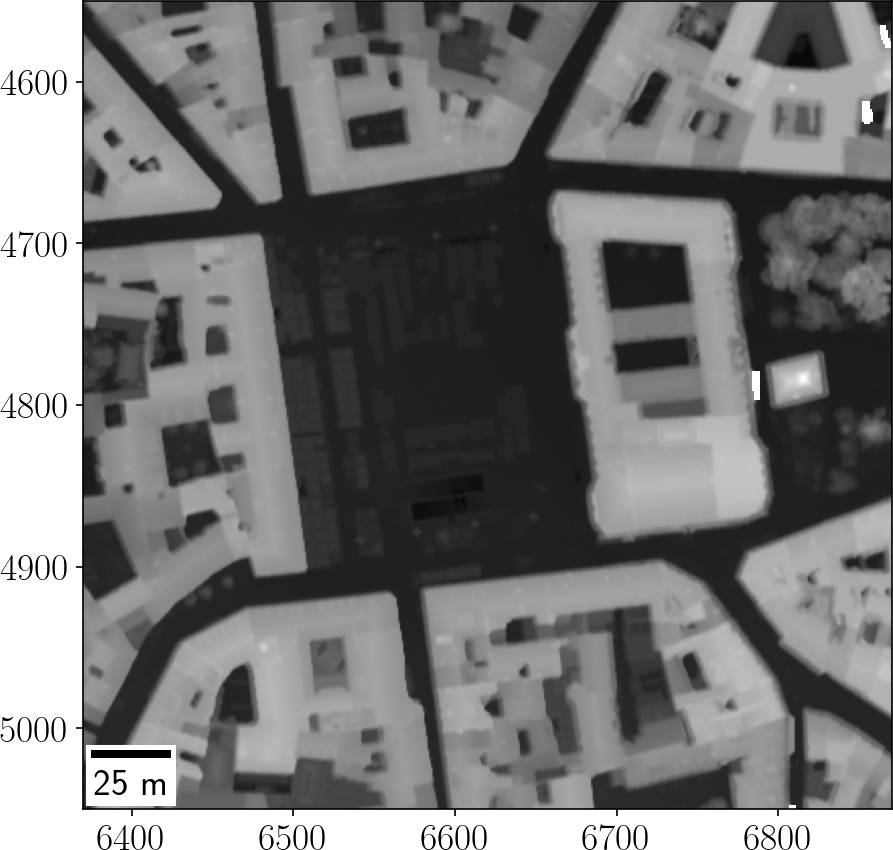
\includegraphics[height=6cm]{Images/Chap_1/DSM_Capitole_LiDAR.png}
        \caption{\acrshort{dsm} from \acrshort{lidar} HD data,\\Place du Capitole}
        \label{fig:DSM_capitole_lidar}
    \end{subfigure}\hfill
    \begin{subfigure}[t]{0.5\linewidth}
        \centering
        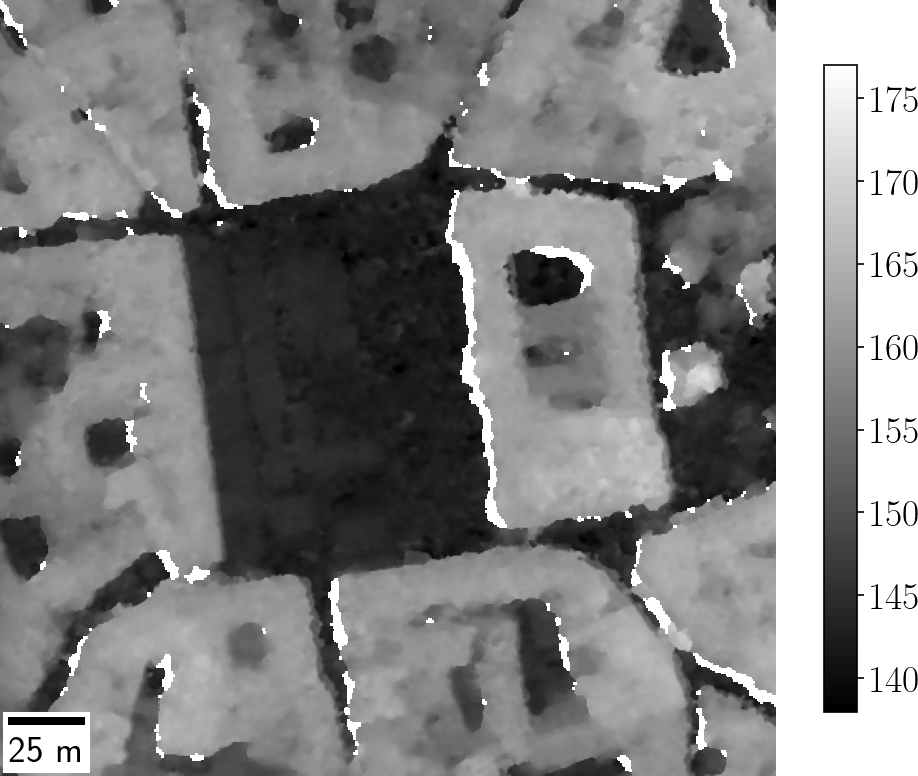
\includegraphics[height=6cm]{Images/Chap_1/DSM_Capitole_CARS.png}
        \caption{\acrshort{cars} \acrshort{dsm} from Pléiades images,\\Place du Capitole}
        \label{fig:DSM_capitole_cars}
    \end{subfigure}
    \begin{subfigure}[t]{0.5\linewidth}
        \centering
        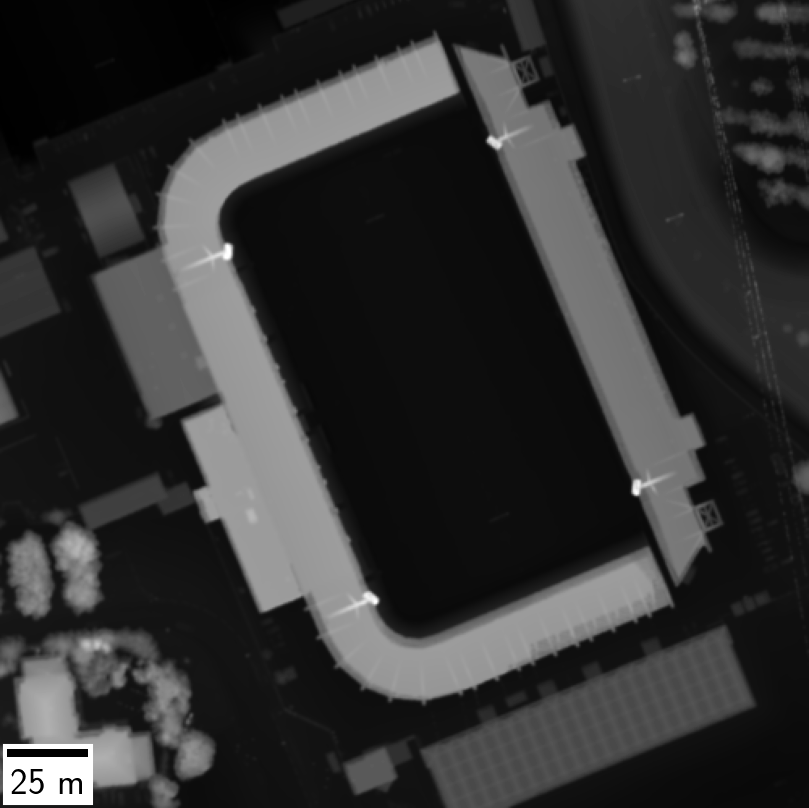
\includegraphics[height=6cm]{Images/Chap_1/DSM_Wallon_LiDAR.png}
        \caption{\acrshort{dsm} from \acrshort{lidar} HD data,\\Ernest Wallon stadium}
        \label{fig:DSM_ernest_wallon_lidar}
    \end{subfigure}\hfill
    \begin{subfigure}[t]{0.5\linewidth}
        \centering
        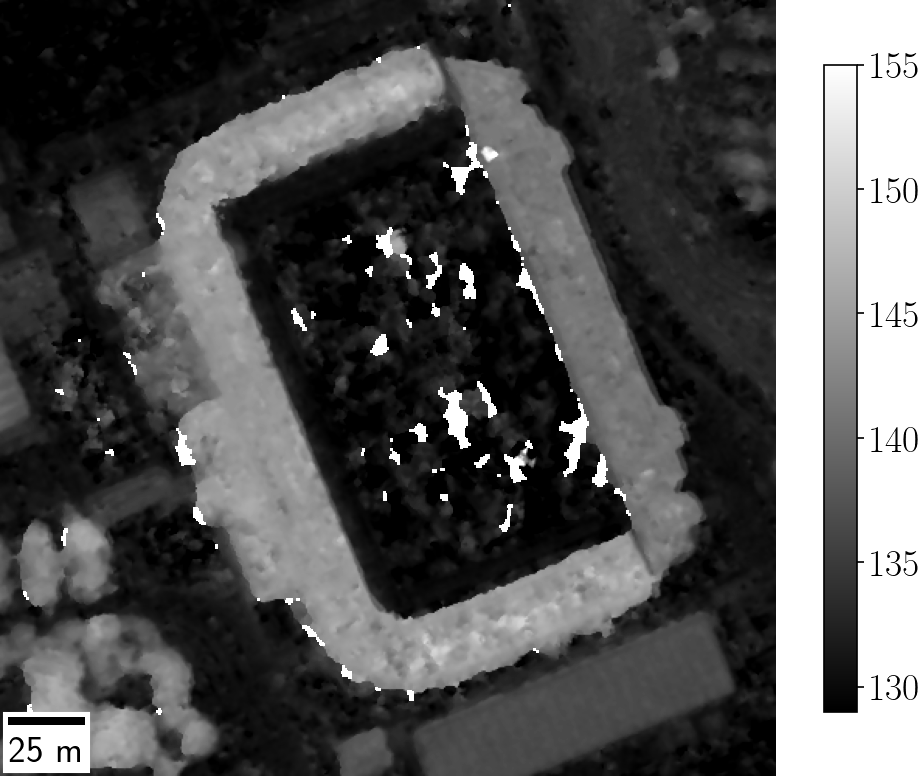
\includegraphics[height=6cm]{Images/Chap_1/DSM_Wallon_CARS.png}
        \caption{\acrshort{cars} \acrshort{dsm} from Pléiades images,\\Ernest Wallon stadium}
        \label{fig:DSM_ernest_wallon_cars}
    \end{subfigure}
    \caption{Different \acrshort{dsm}s over Toulouse, France. \acrshort{dsm}s were obtained by rasterizing \acrshort{lidar} HD data or by processing Pléiades stereo images with the \acrshort{cars} pipeline. The \acrshort{cars} pipeline uses a $5\times5$ CENSUS cost function and \acrshort{sgm} regularization for stereo reconstruction. \copyright \acrshort{cnes} 2017, Distribution AIRBUS DS}
    \label{fig:DSM_toulouse}
\end{figure}

Once the regularized cost volume $C_V^{SGM}$ has been computed, the classical approach in the literature is to apply a \textit{winner-takes-all} strategy to determine the disparity map $\mathcal{D}$:
\begin{align}
    \mathcal{D}(\rowcol) = \argmin_d C_V^{SGM}(row, col, d) 
\end{align}

\subsubsection{Disparity Refinement}\label{sec:postprocess_disparity}
Once the disparity map has been computed, it is usually post-processed to remove artifacts, and improve disparity resolution. It is common to add a sub-pixel refinement step, where a non-integer disparity is interpolated around the selected disparity. The main idea is to interpolate a model through the selected disparity $d=\argmin_\delta C_V(\rowcol, ~\delta)$ and its two direct neighbors. The refined disparity $d_{interp}$ is then defined as the $\argmin$ of this interpolation model. \Cref{fig:sub-pixel_refinement} presents examples of interpolated disparities from  \cite{haller_real-time_2010}, mainly a ``V''-like shape as in \ref{fig:vfit_refinement} and a parabola as in \ref{fig:parabola_refinement}. Carrying out sub-pixel refinement suggests we assume the algorithm can attain a significant level of precision, which is debatable (see \Cref{sec:uncertainty_cars}), as well as the fact that the cost function was sufficiently sampled to be correctly interpolated.

\begin{figure}
    \centering
    \begin{subfigure}[t]{0.5\linewidth}
        \centering
        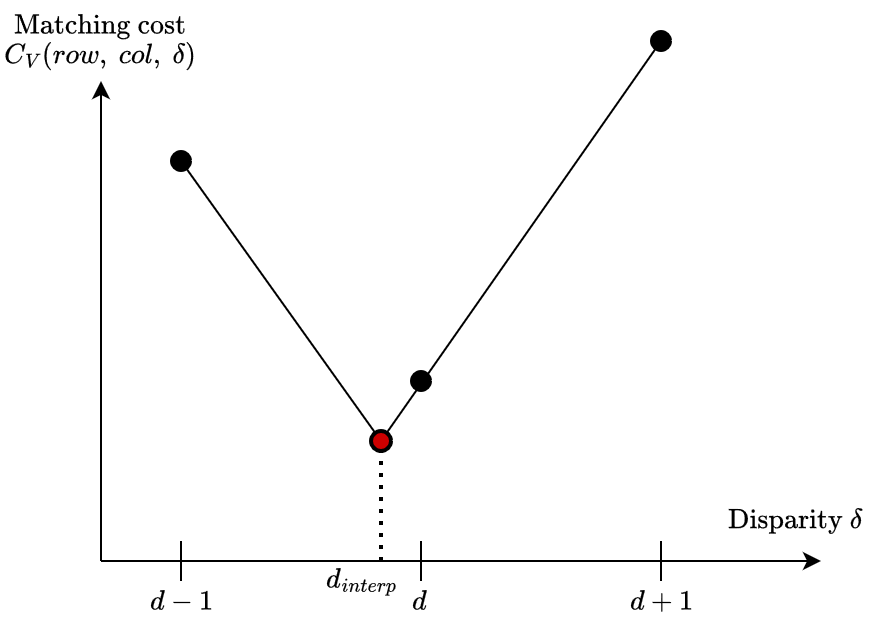
\includegraphics[width=\linewidth]{Images/Chap_1/subpixel_refinment_vfit.png}
        \caption{V-fit sub-pixel refinement}
        \label{fig:vfit_refinement}
    \end{subfigure}\hfill
    \begin{subfigure}[t]{0.5\linewidth}
        \centering
        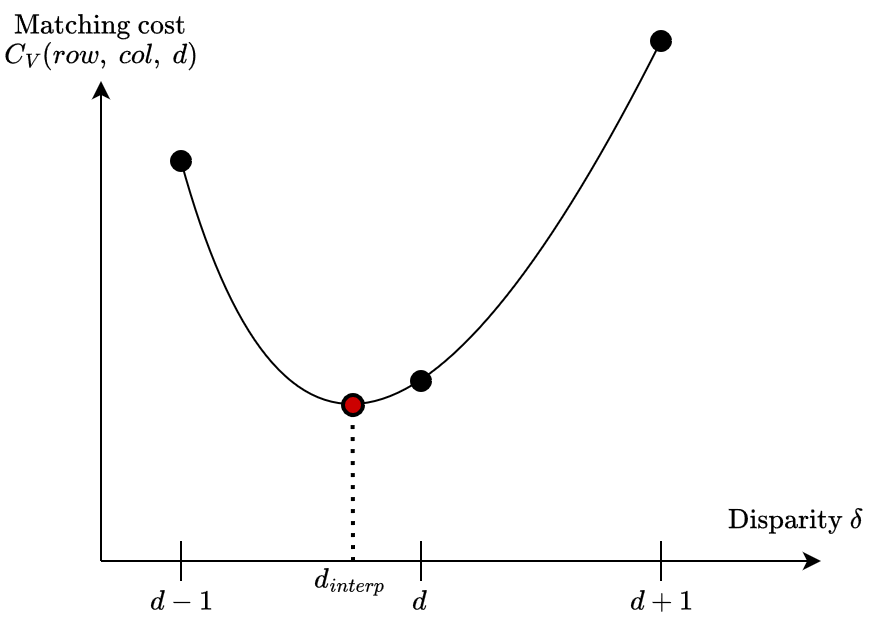
\includegraphics[width=\linewidth]{Images/Chap_1/subpixel_refinment_parabola.png}
        \caption{Parabola sub-pixel refinement}
        \label{fig:parabola_refinement}
    \end{subfigure}
    \caption{Different methods for refining the disparity $d=\argmin_\delta C_V(\rowcol, ~\delta)$}
    \label{fig:sub-pixel_refinement}
\end{figure}

The disparity map can also be filtered in order to remove local outliers. Classical strategies include the use of a mean or median filter for instance. There exists more advance filtering methods, such as bilateral filtering \cite{tomasi_bilateral_1998} which performs a weighted average, where weights depend on the proximity to other pixels both in the spatial and spectral domain.

There exist strategies allowing to detect dubious matches. For instance, cross-checking \cite{fua_combining_1991} verifies if the disparity selected would stay consistent with the one computed by reversing the roles of the images: the reference image becomes the secondary image. We first start by computing a secondary cost volume $C_V'$ by reversing the role of the images. We then obtain two disparity maps $\mathcal{D}$ and $\mathcal{D}'$, and check that they are consistent, as in theory we would that $\mathcal{D}=-\mathcal{D}'$. A pixel $(\rowcol)$ is considered consistent across disparity maps if it verifies:
\begin{equation}\label{eq:cross-checking}
    |\mathcal{D}(row, col) + \mathcal{D}'(row, col+\mathcal{D}(row, col))|\leqslant \tau
\end{equation}
where $\tau$ is a consistency threshold usually set to $1$. For errors that do not satisfy this consistency check, it has been proposed in \cite{hirschmuller_stereo_2008} to differentiate between mismatched pixels and occluded pixels. Mismatch pixels are pixels for which there exists a correct match, whereas occluded pixels are pixels that are visible in an image but masked by an object in the other. The difference is determined as follows: if there is a disparity $d\in\mathcal{D}$ such that $\mathcal{D}'(row, col+d)=-d$ then it is a mismatch. Otherwise, pixel $(\rowcol)$ is occluded. Occluded regions of an image can be filled by interpolation with the closest valid disparities or left as \textit{nodata}.  

\begin{remark}
     \Cref{eq:cross-checking} requires the computation of a second cost volume, which effectively doubles the processing time. As dense stereo matching is also the longest part of a photogrammetry pipeline, one might be reluctant to carry out a cross-checking step. However, we can make the following observation: the cost volume contains the dissimilarity between every considered pair of pixels in the disparity range, so the cost of every considered match in the first cost volume is also present in the second cost volume. In theory, for every pixel $(\rowcol)$ and for every disparity $d$ in the (reference) disparity range, it holds \cite{bebis_mutual_2008}:
     \begin{align}\label{eq:diagonal_search}
         C_V(\rowcol,~d) = C_V'(\rowcol+d, -d)
     \end{align}
     \Cref{eq:diagonal_search} holds only for cost volumes obtained after the matching cost step. However, when \acrshort{sgm} regularization or another aggregation cost method modifies cost volumes, then the there can be differences between $C_V(row,~col,~d)$ and $C_V'(row,~col+d, -d)$. In the case of \acrshort{sgm} regularization, series of tests show that the differences between cost volumes are small and marginally modify the disparity maps. Using \eqref{eq:diagonal_search} then allow to obtain both cost volumes by only computing one and re-indexing it to obtain the other.
\end{remark}

Once every step of the dense matching algorithm have been carried out, the disparity map obtained is used create pairs of lines of sight to triangulate 3D point clouds.

\subsection{Triangulation}\label{sec:triangulation}
The disparity maps allow to deduce elevation information contained in the shift of objects in both image spaces. Computing this information is carried out during the triangulation step of the stereo pipeline.

The type of optical sensor used determines the resolution of the disparity map, and therefore the density of the resulting point cloud. It will therefore influence the planimetric resolution of the final \acrshort{dsm}. We usually consider that the planimetric resolution of the \acrshort{dsm} can be similar to the resolution of the sensors. On the other hand, the altimetric resolution of the \acrshort{dsm} is determined by the altitude and positions of the satellites \cite{qin_critical_2019}. This position can be characterized by the \acrfull{b/h} ratio, as in \Cref{fig:RPC}. This ratio is computed by dividing the distance separating the stereo acquisitions by the altitude of the satellite. It indicates the angle formed between the lines of sight originating from the satellites towards an object of the scene. A high \acrshort{b/h} allows for high elevation accuracy, but possesses more occluded regions (for instance a narrow street between two high buildings), and conversely for a low \acrshort{b/h} \cite{delon_small_2007}. In natural landscapes, stereo acquisitions present high \acrshort{b/h} ratio in order to have a high altimetric accuracy, while the \acrshort{b/h} ratio is smaller in urban landscapes to limit the occlusions.  In our experiments, the \acrshort{b/h} ratio for stereo acquisitions varies between $0.1$ and $0.4$. The \acrshort{co3d} will use \acrshort{b/h} ration between $0.2$ and $0.3$. The \acrshort{b/h} will also partly determine the value of the altimetric ratio $r_{alt}$ presented in \Cref{sec:epipolar_geometry}.

The quality of the final \acrshort{dsm} is also influenced by the solar angles \cite{qin_critical_2019}, with the zenith angle being as small as possible to limit the projected shadows over the scene. Sun-synchronous satellites, such as Pléiades or \acrshort{co3d}, benefit from advantageous sun angles in order to favor good images acquisitions and good stereo reconstruction.

\begin{figure}
    \centering
    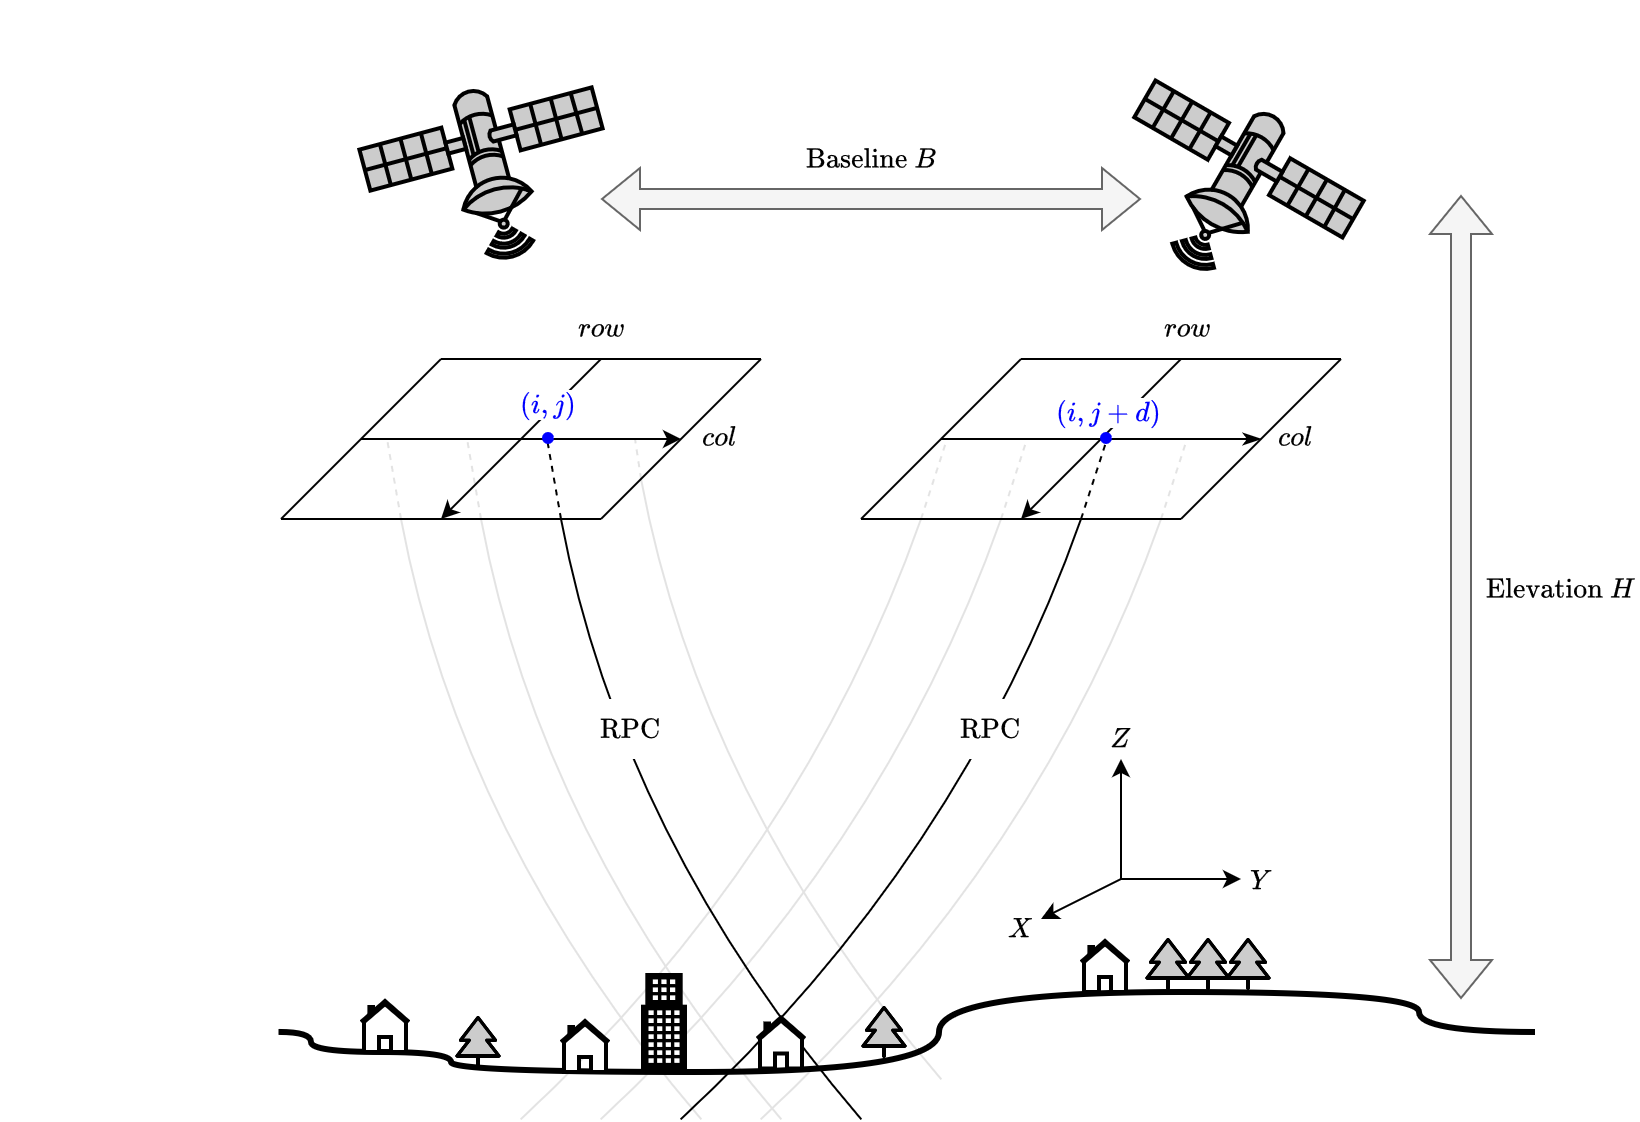
\includegraphics[width=0.8\linewidth]{Images/Chap_1/RPC.png}
    \caption{Triangulation of the position of a point using \acrshort{rpc} models. The distance $B$ between satellites as well as the global elevation $H$ can be used to determine the angle between satellites.}
    \label{fig:RPC}
\end{figure}

The computed disparity map allows to determine the position of 3D points. When working with pinhole camera models, the depth $z$ of a pixel is computed using the following formula:
\begin{equation}
	z=\frac{Bf}{d}\label{eq:z_bfd}
\end{equation}
where $B$ is the baseline between cameras, $f$ is the focal length of the camera, and $d$ is the disparity of a pixel. This formula can be found using optical geometry \cite{bolles_epipolar-plane_1987}, and illustrates the fact that pixels closer to the camera present a bigger position shift in between images. As mentioned previously, the pinhole camera model is not valid in the case of satellite imagery,  and we instead use other sensor models (see \Cref{sec:sensors_rpc}). \Cref{eq:z_bfd} thus cannot be used as such to provide accurate results. The disparity 

Instead, the disparity is used to determine pairs of lines of sight pointing to the same object. Using \acrshort{rpc} models, we can compute the 3D coordinates of every intersection of pairs of lines of sight. To do so, we first consider the \acrshort{rpc} models $\RPC_1$, $\RPC_2$ of two stereo images defined in \cref{eq:rpc}. We consider as well their epipolar grids $g_{e1}$, $g_{e2}$ from \cref{eq:epipolar_grid}. For every pixel $(row_e, ~col_e)$ from the reference epipolar image, whose disparity is $d$, the 3D point $(X, Y, Z)$ represented by $(row_e, ~col_e)$ is the point verifying the following equations:
\begin{align}
    (X, Y, Z) &= \RPC^{-1}_1(g_{e_1}(row_e,~col_e),~Z)\label{eq:triangulation_exact}\\
    (X, Y, Z) &= \RPC^{-1}_2(g_{e_2}(row_e,~col_e+d),~Z) 
\end{align}
If the lines of sight intersect, then $Z$ is found by solving the following equation:
\begin{equation}
     \RPC^{-1}_1(g_{e_1}(row_e,~col_e),~Z) = \RPC^{-1}_2(g_{e_2}(row_e,~col_e+d),~Z) 
\end{equation}
Knowing $Z$ and $g_{e_1}(row_e,~col_e)$, \cref{eq:triangulation_exact} provides the $X$ and $Y$ coordinates as well.

A known problem is that lines of sight rarely intersect. By approximating lines of sight by a starting point $P$ and a direction vector $\overrightarrow{V}$, we can instead define the coordinates $(X,Y,Z)$ as the point minimizing its distance to both lines. Approximating \acrshort{rpc}s by segments is valid on the limited range of considered altitudes. The exact formula for computing $(X,Y,Z)$ is provided in \cite{delvit_geometric_2006}:
\begin{equation}
    (X,Y,Z) = \left[ Id - V_1V_1^T + Id - V_2V_2^T \right]^{-1} \left[ (Id - V_1V_1^T)P_1 + (Id - V_2V_2^T)P_2 \right]
\end{equation}
where $Id$ is the identity matrix, and $V^T$ is the transposed vector $V$. The error due to enforcing \acrshort{rpc}s  intersection is however small (a few centimeters) in comparison to the errors occurring in the disparity map. In this thesis, we mainly focus on processing the disparity errors an therefore do not consider the approximation made during the lines of sight intersection.

Triangulating every point using the disparity map leads to a 3D point cloud. Because we know from which pixel each 3D point originates from, we can associate to every 3D point additional information such as:
\begin{itemize}
    \item The color of the reference pixel (if provided). The point cloud is thus a colored point cloud.
    \item Confidence measures computed during the dense matching step, that will presented in \Cref{sec:uncertainty_pandora}
\end{itemize}

The 3D points can be filtered to remove obvious errors. Advanced filtering methods can be implemented, such as bilateral filtering \cite{digne_bilateral_2017}, and filtering using color information or confidence measures from the disparity map (see \Cref{sec:uncertainty_pandora}) \cite{youssefi_geometrically_2024}. In the \acrshort{cars} pipeline, two different filtering steps are carried out: one for removing statistical outliers, and one for removing so-called ``small-components''.

\subsubsection{Statistical outliers filtering}
Statistical outliers are determined by considering the positions of their neighbors. For each point $P$, we compute the mean distance $\mu_P$ to its $N$ neighbors. Then we can compute for each point $P$ the mean distance $\mu$ and standard deviation $\sigma$ of its $N$ neighbors as:
\begin{align}
    \mu &= \frac{1}{N}\sum_{i=1}^N\mu_i\\
    \sigma &= \sqrt{\frac{1}{N-1}\sum_{i=1}^N(\mu_i-\mu)^2}
\end{align}

A point $P$ is considered to be a statistical outlier if the difference between its mean distance $\mu_P$ and the mean distance $\mu$ of the whole neighboring is too large:
\begin{align}\label{eq:statistical_outlier}
    \mu_P>\mu+k\sigma
\end{align}
Where $k$ is a constant usually set to $5$ by the user. We also consider $N=50$.

\subsubsection{Small-components filtering}
The other filtering method, named small-components filtering, attempts to remove small isolated clusters of points. For each point, we count the number of neighbors $N$ present within a distance $D_{max}$. If this number is inferior to a given threshold $N_{min}$, then we consider the point belongs to a small component and is removed. Formally, a point $P$ is removed if:
\begin{align}\label{eq:small_components}
    \#\{~\text{Points } Q~|~\sqrt{(P-Q)(P-Q)^T}\leqslant D_{max}~\}\leqslant N_{min}
\end{align}
where $\#$ is the cardinal of a set. We usually set $D_{max}$ to $3$m and $N_{min}$ to $50$.

\Cref{fig:point_cloud_filtering} illustrates the two filtering methods presented.

\begin{figure}
    \centering
    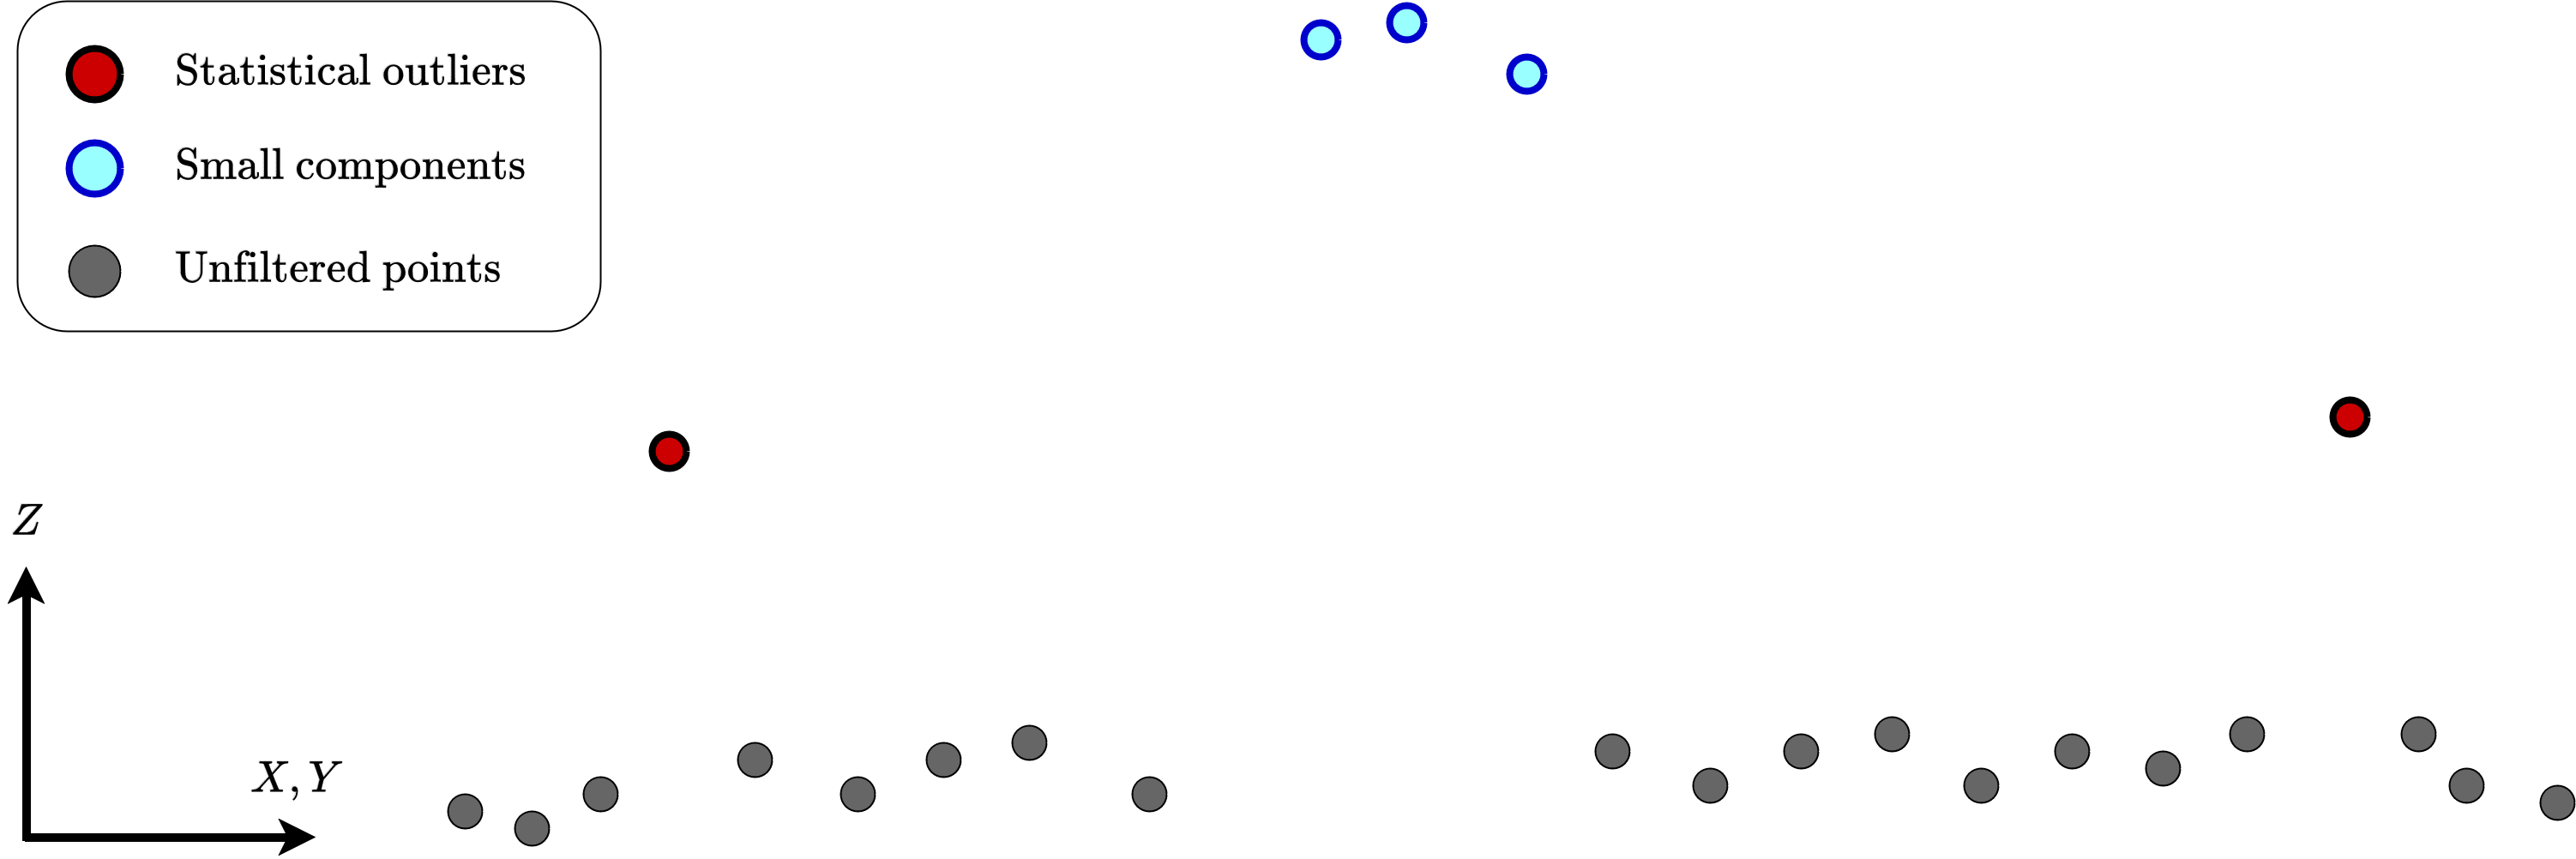
\includegraphics[width=\linewidth]{Images/Chap_1/Point_cloud_filtering.png}
    \caption{Example of statistical outliers and small components filtering of a 3D point cloud.}
    \label{fig:point_cloud_filtering}
\end{figure}

Filtering the point cloud results in a 3D product that can already be provided as such to users. However, point clouds, while containing more 3D information than \acrshort{dsm}s, can be hard to manipulate in conjunction with other \acrshort{gis} data. Projecting the point cloud on a regular grid to produce a \acrshort{dsm} is thus often preferred, which constitutes the final step of the stereo pipeline.

\subsection{Rasterization}\label{sec:rasterization}
Rasterization consists in projecting the 3D points onto a regular grid over the $(X,Y$) plane to produce the final \acrshort{dsm}. One of the challenges faced when projecting the point cloud is that of the low density of the point cloud relative to the \acrshort{dsm} grid. Indeed, if the density of the point cloud is high enough, multiple 3D points can be projected to the same cell, which raises the question on how to merge their 3D information. On the other hand, if the density is too enough, there may be some cells where no points are projected onto. 

The \acrshort{cars} stereo pipeline uses a Gaussian interpolation to fuse the information of point clouds. Given a cell with coordinates $(X,Y)$ of the \acrshort{dsm}, we consider every point $P_i=(X_i, Y_i, Z_i)$ in a given radius $r$ of $(X,Y)$, and note $\mathcal{N}_{XY}$ the set of all those points. The final value of the \acrshort{dsm} is then computed as the following mean with Gaussian weights:
\begin{align}\label{eq:rasterization}
    \DSM(X,Y) &= \frac{\sum_{P_i\in\mathcal{N}_{XY}}Z_i\cdot e^{-\frac{(X_i-X)^2+(Y_i-Y)^2}{2\sigma^2}}}{\sum_{P_i\in\mathcal{N}_{XY}} e^{-\frac{(X_i-X)^2+(Y_i-Y)^2}{2\sigma^2}}}
\end{align}
with $\sigma$ usually set to $0.3$m and the radius $r$ being $3$m. \Cref{fig:rasterization} illustrates the rasterization process.

Rasterizing with this method provides the advantage of smoothing the potential height variations still present in the 3D point cloud, while allocating more weight to points that are near the cell center. This method can also be found in other stereo pipelines \cite{shean_automated_2016}, while other pipelines use different weighting methods, such as Inverse Distance Weightings (IDW) \cite{rupnik_micmac_2017}, producing similar results.

\begin{figure}
    \centering
    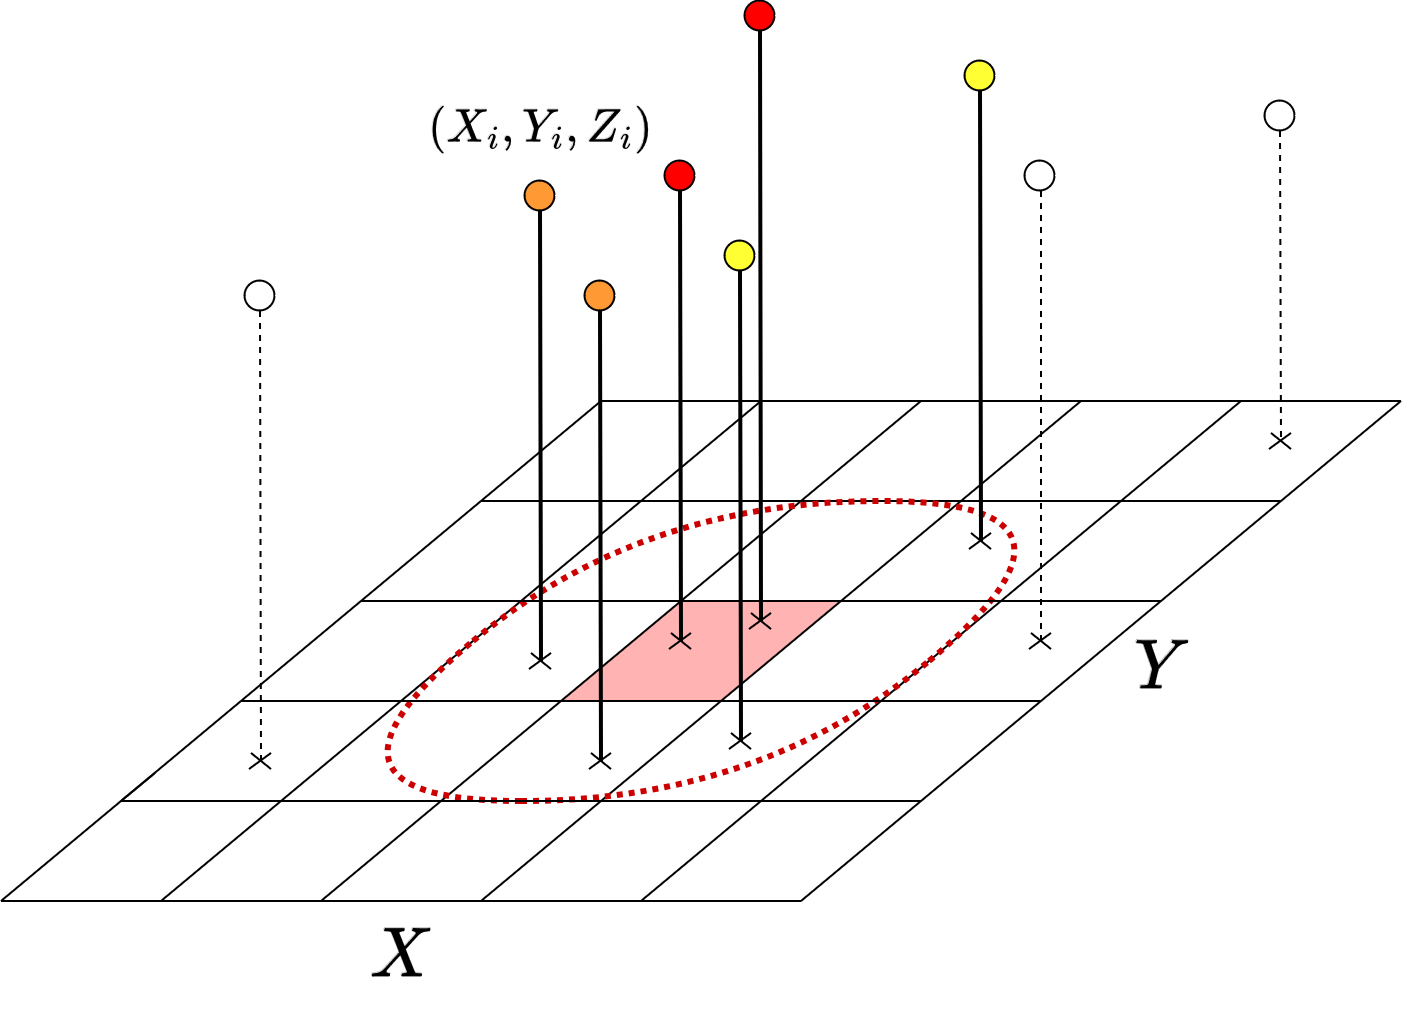
\includegraphics[width=0.7\linewidth]{Images/Chap_1/Rasterization.png}
    \caption{Rasterization of the point clouds on a regular grid. Red points are nearer to the center $(X,Y)$ of the considered cell, while yellow points are further away.}
    \label{fig:rasterization}
\end{figure}

\begin{remark}
    If no points are projected in a given cell (or its direct neighbors), then the cell can be filled with \textit{nodata} values. Different method can be considered to fill holes, such as directly using the values of nearest valid neighboring cells, or interpolating their values. More advanced methods consists in simulating a cloth-like surface fill the holes as in \cite{lallement_bulldozer_2022}.
\end{remark}

As we seen in the previous sections, a photogrammetry pipeline consists in multiple processing steps with intermediary products. For each step of the pipeline, different methods (\eg matching, filtering \etc), parameterization and post-processes are available for each step. This broad range of solutions allow to adapt our processes to the type of images and terrain observed, but it sometimes makes it difficult to determine the configuration producing the best quality \acrshort{dsm}, or to single out a general good-working configuration. The values of the different step parameters presented previously, and that we will be using throughout this thesis, result from testing and sensitivity analyses. In this thesis, we will therefore not discuss their value and instead focus on quantifying and propagating the uncertainty of the \acrshort{cars} stereo pipeline.

\section{Uncertainty in Stereophotogrammetry}\label{sec:previous_work_stereo_uncertainty}
Producing high resolution \acrshort{dsm}s is a complex task, where many uncertainties arise. Those uncertainties can be associated with input data (noise on images, sensor model location uncertainty) or be caused by the processing of those data (resampling errors, disparity computation, rasterization method).

We will first look at attempts to characterized the uncertainty associated with \acrshort{dsm}s.

\subsection{Related Work}\label{sec:related_work}
The quality of \acrshort{dsm} can greatly vary depending on the quality/resolution of the data used, the precision of the geolocation, the performances of the processing algorithm \etc.

From a product point of view, such as TanDEM-X for instance, quality masks can be provided alongside the \acrshort{dem}, usually based on the sensor or method used for producing the \acrshort{dem}. TanDEM-X produces a height error map \cite{wessel_tandem-x_2018}, representing for each DEM pixel the standard deviation corresponding to the height error. The value is derived from the interferometric coherence, and is considered to be a stochastic error. It does not include any contributions of epistemic errors, such as erroneous orbital parameters. The altimetric and planimetric accuracy of by \acrshort{ign}'s \acrshort{lidar} HD 3D points have been measured using ground control points (25cm of planimetric relative accuracy, 5cm of altimetric relative accuracy). Other intrinsic quality parameters of the \acrshort{ign}'s \acrshort{lidar} HD numerical models have not been measured \cite{ign_lidar_2024}. However, \acrshort{ign}'s \acrshort{dtm} product, the RGE ALTI®, possesses a mask indicating the quality of the data provided. This quality mask is composed of the data source used (\acrshort{lidar}, stereo photogrammetry, \acrshort{radar}) for which the mean squared altimetric error has been determined for each source \cite{ign_rge_alti_2013}. In particular, the photogrammetry altimetric accuracy is estimated between 1.5 and 2.5m according to \cite{ign_bd-topo_2013}.

Other work try to estimate the uncertainty associated with a \acrshort{dsm} based not on the method or sensor used, but on the values of the \acrshort{dsm} itself. \cite{mesa-mingorance_accuracy_2020} reviews those different methods for assessing the accuracy of \acrshort{dsm}s. They are mostly producing confidence intervals associated with a \acrshort{dsm} \cite{oksanen_digital_2006,panagiotakis_validation_2018,deschamps-berger_apport_2021}. Those work use robust estimators to evaluate the mean, median and variance of a \acrshort{dsm} altitude distribution \cite{wang_robust_2015}, or advanced statistical methods such as variograms to measure the spatial correlation of errors \cite{hugonnet_uncertainty_2022}. Using those methods, it is possible to produce a confidence interval that globally describes the uncertainty associated to a given \acrshort{dsm} (or a single interval per slope category in \cite{hugonnet_uncertainty_2022}). Those methods estimate the uncertainty \textit{a posteriori}, meaning that they do not consider the means by which the \acrshort{dsm} was created. The uncertainty is estimated using a set of reference points, either extracted from a better resolution \acrshort{dsm}, or from GPS ground control points. In \cite{wang_robust_2015}, the confidence intervals are computed based on the residuals between the \acrshort{dsm} and a bilinear interpolation of samples from the same \acrshort{dsm}, supposing that the quality of a \acrshort{dsm} can be evaluated without using an external reference. 

Photogrammetry pipelines presented in \Cref{sec:different_photogrammetry_pipelines} also have different methods of estimating the uncertainty of the produced \acrshort{dsm}s. For instance, the NASA's ASP pipeline can take as inputs camera planimetric standard deviation of position uncertainty (expressed in meters), and propagate it during the triangulation and rasterization steps. The documentation \cite{nasa_ames_2020} details the covariance matrix propagation method used. It explicitly states that the propagated uncertainty does not represent the error between the predicted height and a hypothetical ground truth, even though they are expressed in the same unit of measure. It is rather the propagated covariance from the camera position projected in the horizontal and vertical directions, regardless of the matching errors or triangulation errors. We did not find clear documentation on how the S2P pipeline handles uncertainties, but the available code of the algorithm suggests that a confidence measure can be computed during the dense matching step of the algorithm (presented later in \Cref{sec:uncertainty_pandora}) and provided alongside the final \acrshort{dsm} as a quality mask. The confidence measure used is a measure of the consensus between the different regularized directions during the \acrshort{sgm} regularization. It is thus an dimensionless parameter, indicating if the predicted height is confident or not.  \acrshort{ign}'s MicMac software computes different errors such as the residual errors from Bundle Adjustment step \cite{ign_micmac_2022}, and provides a correlation map alongside the \acrshort{dsm}. SETSM also computes matching scores \cite{noh_surface_2017}, but it does not seem to be propagated until the final \acrshort{dsm}. DLR's CATENA code is not available, and no documentation indicates the existence of a quality map. In any case, it seems as most pipelines compute a confidence measure (usually during the dense matching step) and propagate it to create a quality mask alongside the final \acrshort{dsm}. This quality mask produced indicate the amount of confidence associated with each \acrshort{dsm} cell value, but does not indicate its potential altimetric error. 

To the best of our knowledge, there is currently no method for producing elevation confidence intervals at a pixel level, by opposition to the global or almost global intervals in \cite{oksanen_digital_2006,wang_robust_2015,hugonnet_uncertainty_2022}. Furthermore, the uncertainty arising from the different photogrammetry algorithms are not considered when producing those intervals. The main contribution of this thesis is the production of pixel-wise confidence intervals for \acrshort{dsm}s produced by photogrammetry. In the following section, we present different sources of uncertainty present in the \acrshort{cars} pipeline. 

\subsection{Uncertainty in the CARS pipeline}\label{sec:uncertainty_cars}
In this thesis, we focused on quantifying the uncertainty alongside the creation process of \acrshort{dsm}. We thus differ in this regard from previous work, which produces a single confidence intervals from the final produced \acrshort{dsm}. Multiple sources of uncertainty influence the production of a \acrshort{dsm}, which we will now detail.

A first source of uncertainty comes from the input data, \ie the radiometric uncertainty associated with stereo images and the geometric uncertainty associated with sensors models. The radiometric uncertainty is mainly due to noise from the sensor and from atmospheric effects appearing on the acquisitions. Those radiometric errors can be estimated and are relatively moderate \cite{jacobsen_radiometric_2014}. Regarding the uncertainty associated with the sensor models, satellite movements not captured by models can have a big impact on the final images, especially for push-broom sensors. For instance, vibration of the satellite can lead to biases on the geolocation of the different rows of the image. Those biases will themselves be propagated to the final \acrshort{dsm}, leading to errors of a few meters \cite{loghin_accuracy_2019}. Additionally \acrshort{rpc} models attempt to represent real lines of sight with polynomial coefficient, which is not exact and possess its own accuracy. The method used for coefficients calibration and the frequency of calibration also bring their share of uncertainty. 

Another source of uncertainty arises from the different processing steps of the stereo pipeline. First, different resamplings occur in order to convert stereo images from sensor geometry to epipolar geometry one. Those resamplings are based on \acrshort{sift} matches, presented in \Cref{sec:epipolar_geometry}. \acrshort{sift} matches are used to refine the epipolar grid depend on the performance of the \acrshort{sift} algorithm used to obtain them. In homogeneous and texture-less area, \eg glaciers, false matches can arise. This leads to wrong epipolar lines, themselves preventing correct results in the dense matching step and leading to a false 3D reconstruction.  We assume in this thesis that the refinement of epipolar grids using \acrshort{sift} points, which minimizes the mean error, provides accurate epipolar resampling grids with an epipolar error of around a tenth of a pixel \cite{franchis_automatic_2014}. However, the resampling in epipolar geometry introduce errors if the input and target resolutions do not respect Shannon criteria \cite{delon_small_2007}. In the case of Pléiades images, the acquisition resolution is usually high enough to insure correct resampling \cite{jacobsen_radiometric_2014}. 

The resampled images in epipolar geometry are then used as inputs for the dense matching step. Dense stereo matching is a complex task, for which many different algorithms exist, each potentially presenting different performances. When compared to epipolar errors, that typically are less than a pixel \cite{franchis_automatic_2014}, dense matching errors can potentially reach higher magnitudes, depending on the size of the considered disparity range (sometimes reaching hundreds of pixels). Considering those orders of magnitude, estimating and quantifying the uncertainty of the stereo matching process is therefore crucial to control the uncertainty on the output \acrshort{dsm}. Some of the sources of those errors are now presented. Because the correlator usually compares windows (in our case $5\times5$ windows using the CENSUS cost function or $11\times11$ windows using MC-CNN) and not single pixels, this can create an adherence effect near building borders, as in \Cref{fig:adherence_window}. Note that in \cite{okutomi_stereo_1994}, authors have been trying to adapt the window shape to reduce the uncertainty of stereo matching, but this method requires to iteratively compute costs on different windows, which can become quite expensive. Using a window-based correlator with \acrshort{sgm} regularization, if correctly parameterized, usually presents good performance in areas without height discontinuities. This can become a problem in urban areas, where the presence of high buildings represents an additional challenge for the correlator. As \acrshort{sgm} regularization also penalizes disparity changes, tops of buildings tend to be extended beyond their true footprint. Other processes, such as filtering or sub-pixel refinement, improve the quality of the disparity map but require specific care for handling their induced uncertainty. \Cref{sec:uncertainty_pandora} dives more into details regarding the different methods that have been developed to quantify the uncertainty of dense stereo matching.

Once the disparity has been estimated, 3D points can be triangulated by intersecting \acrshort{rpc} lines from each matched pixel. However, we saw previously that there is no guarantee that the 3D lines do intersect. If they indeed do not intersect, the 3D point is defined as the point minimizing its squared distances to both lines of sight. An alternative is to modify the geolocation line from the secondary image so that it intersects the line from the reference image. In both cases, the localization of the 3D point is not exact. This uncertainty stems from the fact that \acrshort{rpc} have a their own limited resolution, and that stereo images (resampled or not) do not necessarily point to the exact same location in the object space.

The final part of the stereo pipeline is to rasterize the point cloud onto a regular grid, thus yielding the \acrshort{dsm}. When characterizing the uncertainty on the final result, we must first agree on what the \acrshort{dsm} is assumed to represent. It is common to consider that each pixel's value should represent the average height over the cell. However, providing the maximum or minimal height might be more adapted to some scenarios: for instance if the \acrshort{dsm} is used to prepare very low altitude flights (for drones \etc), the maximum height is more relevant as one would want to avoid any foliage or power line. Those elements could disappear in the final \acrshort{dsm} if it represented the mean or median elevation. In this thesis, we will consider that the \acrshort{dsm} represents the (weighted) average height. Depending of the resolution of input images and the desired output resolution of the \acrshort{dsm}, the density of points per \acrshort{dsm} cell will vary. In our applications, the input and output resolutions are identical as we typically desire to produce a \acrshort{dsm} at $50$cm resolution from $50$cm panchromatic images. This means that there is on average one 3D point per \acrshort{dsm} cell. For occluded regions, or when we discarded stereo matches that seemed incorrect, there might be no point directly in the output cell. In this case, the value of the \acrshort{dsm} cell will be completely determined by the value of points in neighboring cells, even if their distance is high and the averaging weights are small. Interpreting the final \acrshort{dsm} as the average height on each cell is thus debatable, as the average is computed on a limited number of points, and sometimes not even belonging to the considered cell. Note that if there is no points around in a given radius, the cell will be left empty. 

Different sources of uncertainty occurring throughout the stereo pipeline were presented in the previous paragraphs. Characterizing, modelling and propagating all of those uncertainties could not be considered in the span of this thesis. We thus focus mostly on the uncertainty arising from the dense stereo matching step, as it is the source of the biggest errors in the pipeline. \Cref{chap:propagating} investigates how uncertainty from the input epipolar images can be propagated in the stereo matching step, and \Cref{chap:epistemic_uncertainty} attempts to model the processing uncertainty of stereo algorithm itself. We also propagate this uncertainty all the way to the output \acrshort{dsm} and show that it can correctly estimate the errors made during the \acrshort{dsm} production.

\subsection{Uncertainty Quantification in Dense Stereo Matching}\label{sec:uncertainty_pandora}
As stereo matching is a popular problem in computer vision, many methods for quantifying its uncertainty have been proposed in the literature. Without being exhaustive, this section presents a quick overview of the main approaches as well as the solutions currently implemented in the dense stereo correlator Pandora used in the \acrshort{cars} pipeline.

The way uncertainty is quantified in stereo matching is mainly done by producing \textit{confidence maps}, \ie a mapping for each pixel $(\rowcol)$ to a real confidence value, usually between $0$ and $1$. By convention, a value of $0$ means that we are not confident in the disparity value associated to $(\rowcol)$. Conversely, a confidence value of $1$ indicates that we are very confidence in the predicted disparity.

There are multiple sources of information that can be used to compute a confidence measure. Left and right input images and the predicted disparity map being those available to every method, but cost-based approaches can also make use of the cost volume, as it contains a quantity of useful information. Most confidence measures are handcrafted using those different information sources. For reviews on those methods, we refer to \cite{egnal_stereo_2004, hu_quantitative_2012, poggi_quantitative_2017}. With the rising use of deep-learning in stereo, many networks have also been developed to estimate the uncertainty. A review for methods using regression forests can be found in \cite{min-gyu_park_leveraging_2015}, and a more general review, including the use of 2D and 3D CNNs on the cost volume, can be found in \cite{poggi_confidence_2021}.

\begin{remark}
     Quantifying the uncertainty in stereo matching is a popular field of research. Recently, people have even been trying to evaluate the uncertainty of the confidence estimation itself, called \textit{meta-confidence} \cite{kim_meta-confidence_2022}.
\end{remark}

In \Cref{ex:confidence_measure}, we present some examples of confidence measures that use different sources of information.

\begin{example}\label{ex:confidence_measure}
    Regarding confidence measure based on the disparity map, we already presented a type of binary confidence measure in \Cref{sec:postprocess_disparity} with the cross-checking test from \cref{eq:cross-checking}. Other methods compute for instance the local variance of the disparity map, where a low variance suggests confident regions.
    
    For methods using the cost volume, a simple method for measuring the cost would be using the value of the matching score measure (MSM, \cite{egnal_stereo_2004}) for a given disparity at coordinates $(\rowcol)$:
    \begin{equation}
        MSM(\rowcol) = -C_V(row, col, \mathcal{D}(\rowcol))
    \end{equation}
    This measure can be normalized between $0$ and $1$ using the global minimum and maximum of the cost volume. The idea behind this measure is the following: a high matching cost for a selected disparity indicates that the two matched pixels are not that similar, and thus the match is not confident. Other measures using the matching cost compare the value of the first and second minimum of a cost curve, or measure the curvature of the cost curves. More advances measures make use of 3D CNNs on the entirety of the cost volume to learn an efficient confidence measure \cite{mehltretter_cnn-based_2019}.
    
    Measures based on the input images usually measure the gradient \cite{haeusler_ensemble_2013} or variance \cite{park_learning_2019} of input images. High gradient or high variances indicate highly-textured regions, which are often easier to match. The confidence is therefore higher for those pixels. 
    
    Deep-learning approaches can combine multiple sources of information (input images, cost volume, disparity map) to learn a confidence measure \cite{tosi_beyond_2018, kim_adversarial_2020}.
\end{example}


\begin{figure}
    \centering
    \begin{subfigure}[t]{0.5\linewidth}
        \centering
        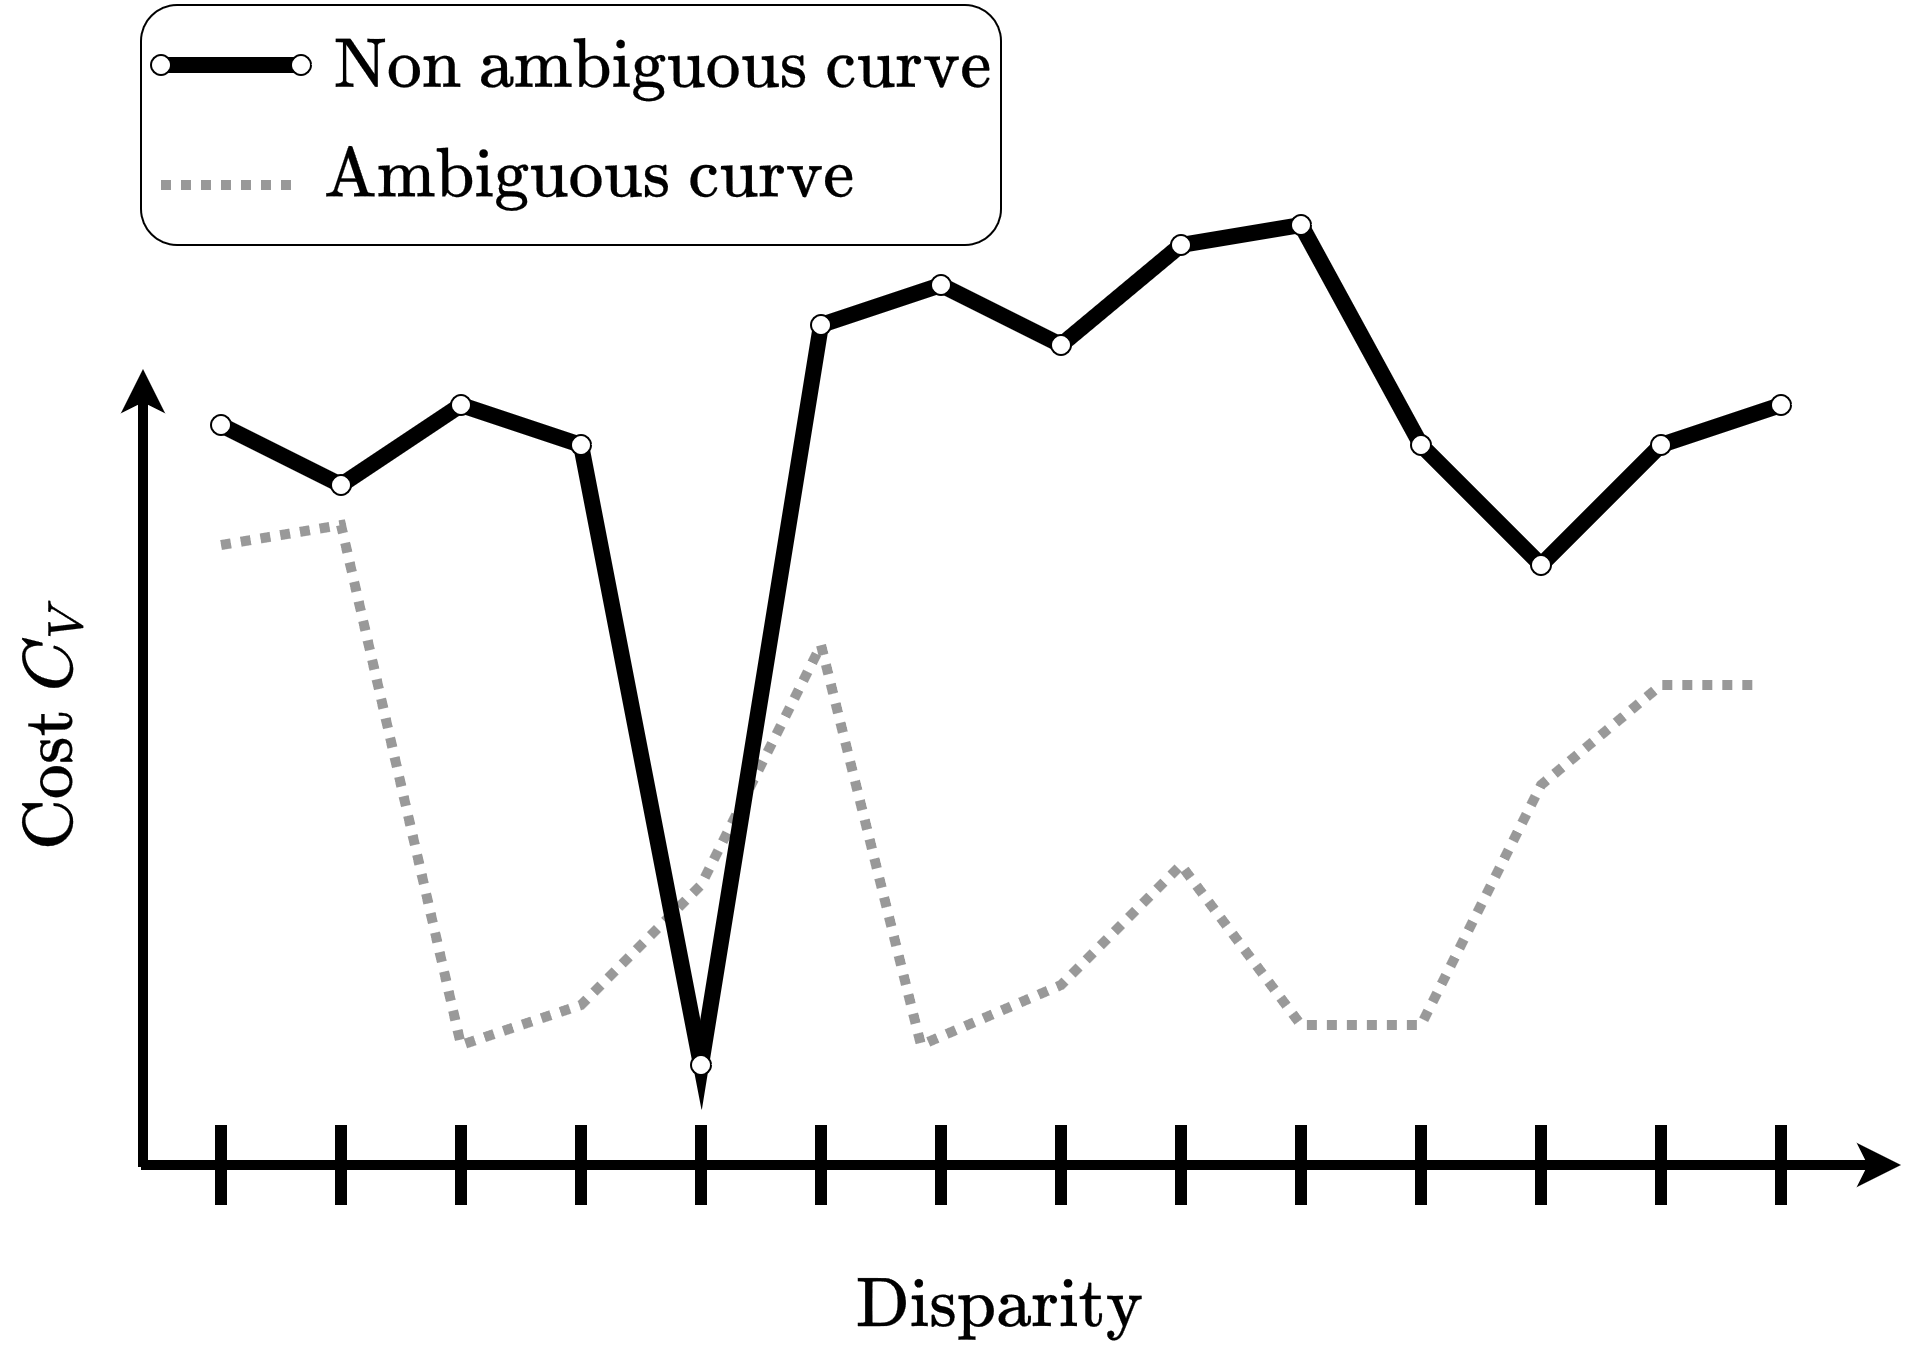
\includegraphics[width=\linewidth]{Images/Chap_1/Ambiguity.png}
        \caption{}
        \label{fig:ambgiuity}
    \end{subfigure}\hfill
    \begin{subfigure}[t]{0.5\linewidth}
        \centering
        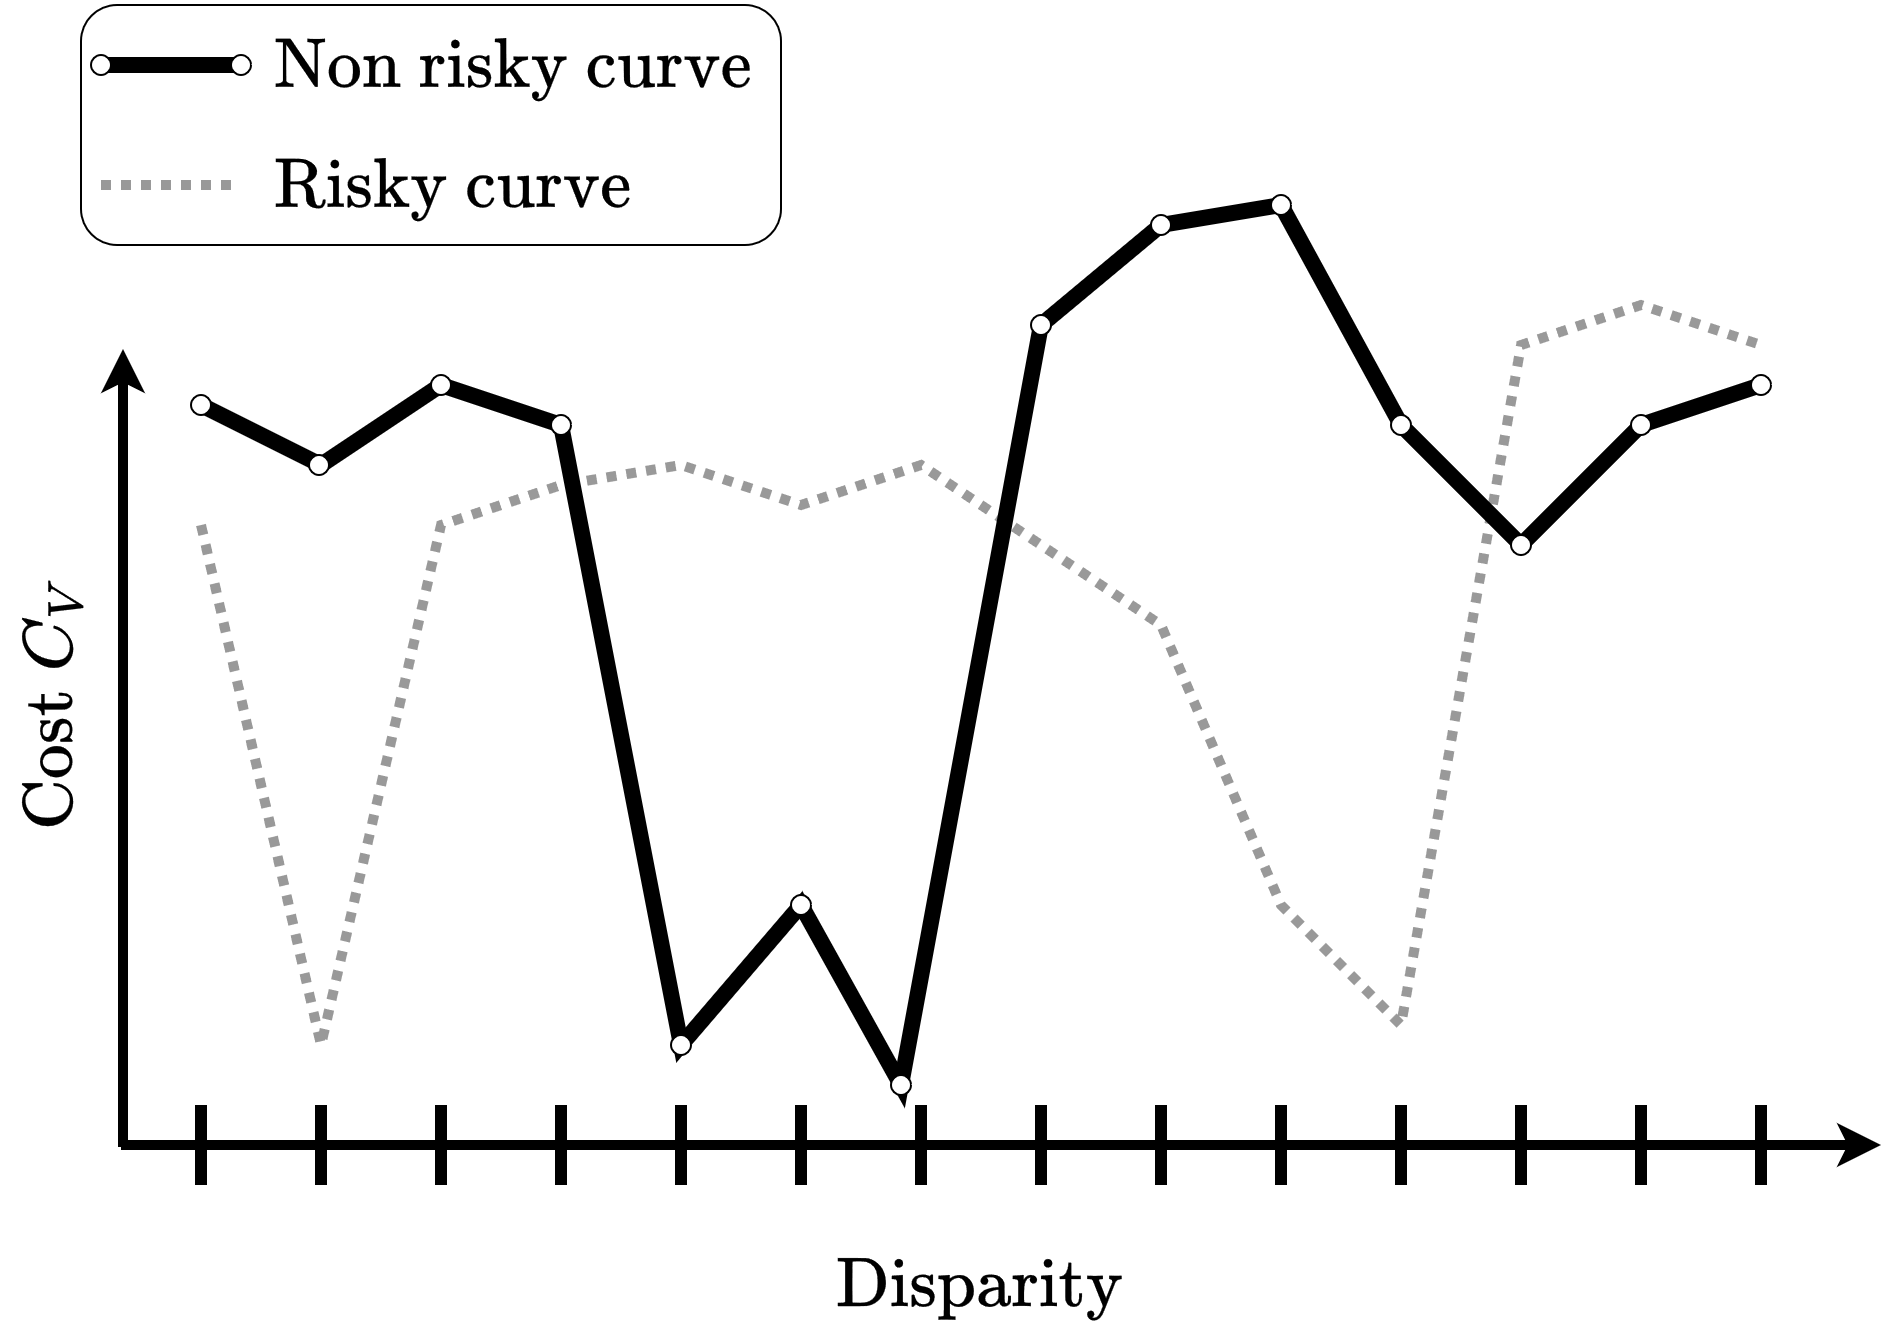
\includegraphics[width=\linewidth]{Images/Chap_1/Risk.png}
        \caption{}
        \label{fig:risk}
    \end{subfigure}\hfill
    \caption{Cost curves with different levels of ambiguity \ref{fig:ambgiuity} and risk \ref{fig:risk}}
    \label{fig:ambiguity_risk}
\end{figure}

In this thesis, we will also consider another confidence measure that can already be computed with the Pandora correlator. This measure will help us to quantify the uncertainty in the photogrammetry pipeline. This confidence measure is a confidence measure called \textit{confidence from ambiguity} \cite{sarrazin_ambiguity_2021}. This method is based on the cost volume and quantifies how easy or hard it is to single out the correct disparity in a cost curve. \Cref{fig:ambgiuity} presents two cost curves, one which is not ambiguous as there is a single well defined minimum, and an ambiguous cost curve which presents multiple values that are close to the minimum. To compute it, we first start by constructing what is called an \textit{ambiguity curve}. We do that by counting how many disparities have a cost close within a threshold $\eta$ to the minimal cost, for increasing values of $\eta$. Formally we need to define for a pixel $(\rowcol)$ the set of all disparities whose cost is within a range $\eta$ of the minimal cost, and then define the ambiguity curve as the cardinal of this set:
\begin{align}
    &\mathcal{D}_\eta = \{d ~|~ C_V(row,~col,~d) \leqslant \min_\delta C_V(\rowcol, ~\delta) + \eta\}\\
    &Amb(\rowcol, ~\eta) = \#\mathcal{D}_\eta
\end{align}
where $\#$ is the cardinal of a set. Evaluating $Amb$ for different $\eta$ gives the ambiguity curve. \Cref{fig:integral_ambiguity_1} presents a cost curve with different values of $\eta$. \Cref{fig:integral_ambiguity_2} presents the resulting ambiguity curve. On those two figures we can see for instance that for $\eta_3$ there are $6$ disparities whose cost is lower than $\min_\delta C_V(\rowcol, ~\delta) + \eta_3$. For non-ambiguous cost curves, $Amb$ will increase only for high values of $\eta$. On the contrary for ambiguous curves, $Amb$ will be high for small values of $\eta$. To obtain a scalar value from $Amb$, we compute the area under its curve, normalized by the range of $\eta$:
\begin{equation}
    \mathrm{AUC}_{Amb}(\rowcol) = \frac{1}{\max\eta-\min\eta}\int_\eta Amb(row,~col,~\eta)d\eta
\end{equation}
It results on low values for confident (non-ambiguous) cost curves, and high values for less confident (ambiguous) curves. Because confidence measures actually present high values for confident pixels, $\mathrm{AUC}_{Amb}$ is normalized and inverted in order to obtain the confidence from ambiguity $c_{Amb}$:
\begin{equation}\label{eq:confidence_from_ambiguity}
    c_{Amb}(\rowcol) = \frac{\max \mathrm{AUC}_{Amb}- \mathrm{AUC}_{Amb}(\rowcol)}{\max \mathrm{AUC}_{Amb} -\min \mathrm{AUC}_{Amb}}
\end{equation}
This way, values of $c_{Amb}$ near $0$ indicate that we are not confident in the predicted disparity. Reversely, values of $c_{Amb}$ near $1$ indicate that we are confident in the predicted disparity.

\begin{figure}
    \centering
    \begin{subfigure}[t]{0.6\linewidth}
        \centering
        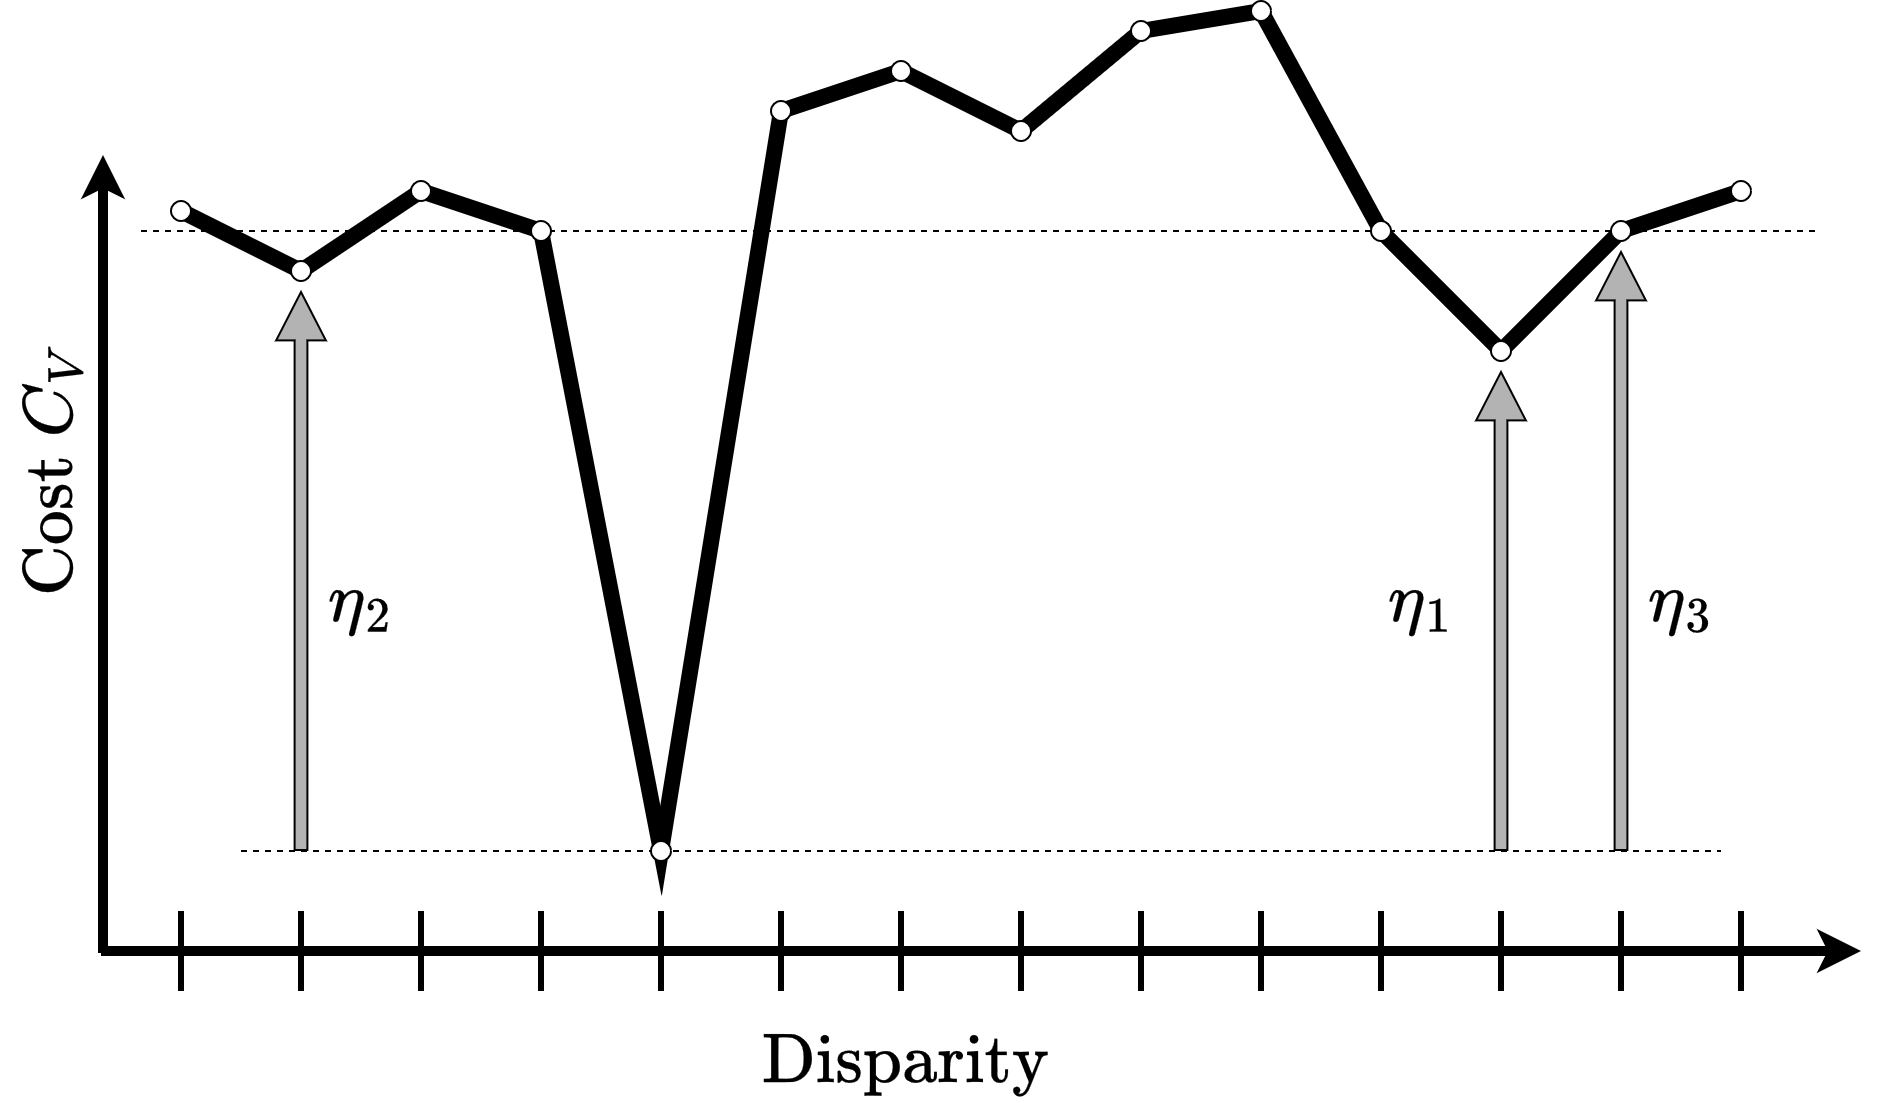
\includegraphics[width=\linewidth]{Images/Chap_1/Integral_Ambiguity_1.png}
        \caption{Cost curve with different values of $\eta$. Horizontal dotted lines indicates the range of costs between $\min_\delta C_V(\rowcol, ~\delta)$ and $\min_\delta C_V(\rowcol, ~\delta)+\eta_3$}
        \label{fig:integral_ambiguity_1}
    \end{subfigure}\hfill
    \begin{subfigure}[t]{0.4\linewidth}
        \centering
        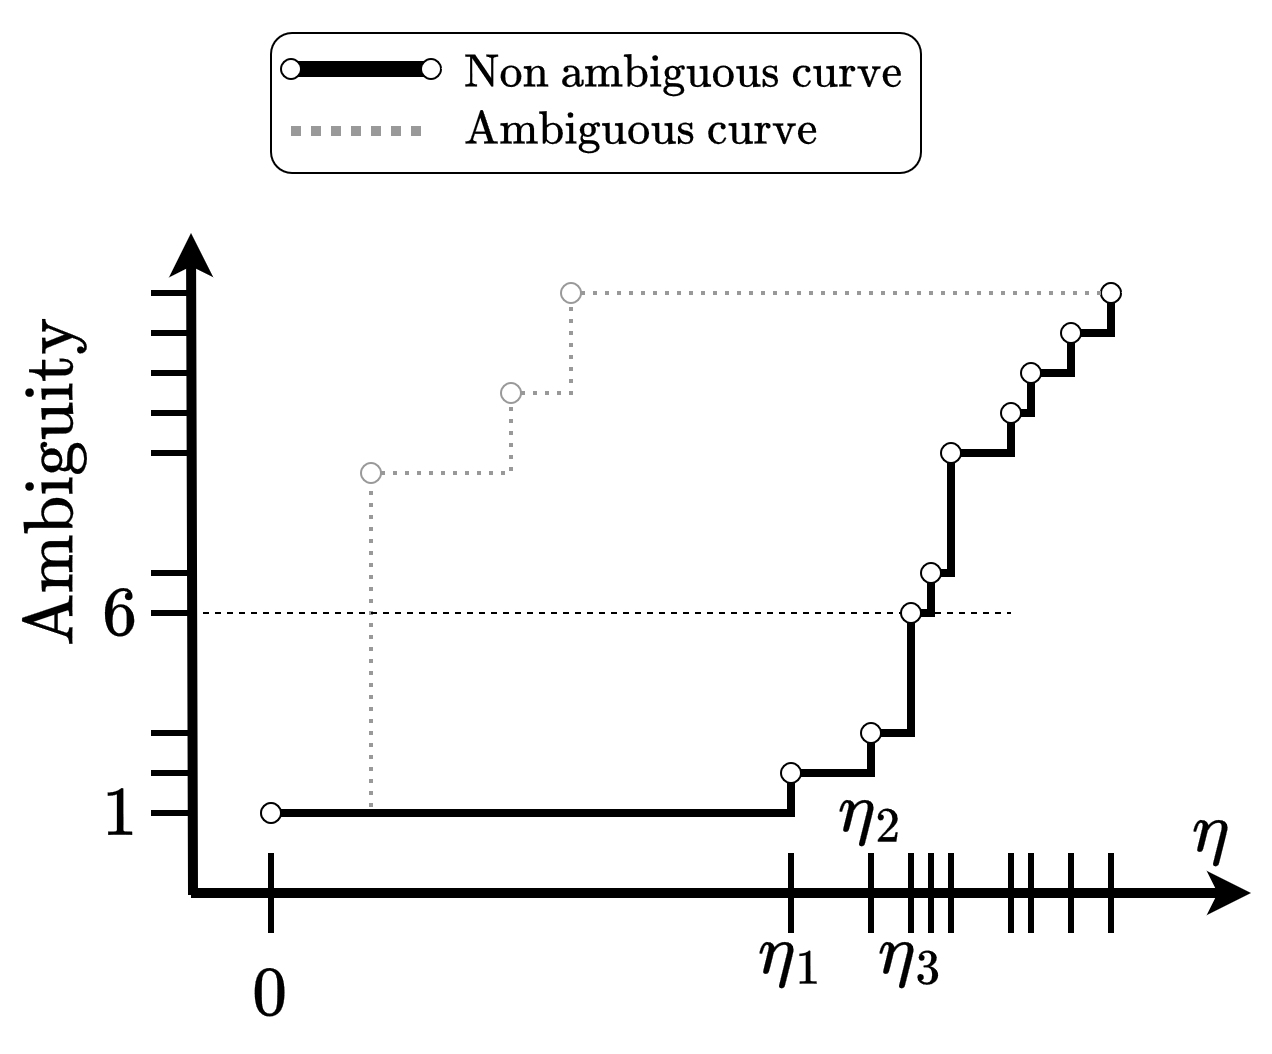
\includegraphics[width=\linewidth]{Images/Chap_1/Integral_Ambiguity_2.png}
        \caption{Associated ambiguity curve in full line. Ambiguous curve in gray dotted line}
        \label{fig:integral_ambiguity_2}
    \end{subfigure}\hfill
    \caption{Illustration of the computation of the ambiguity curve.}
    \label{fig:integral_ambiguity}
\end{figure}

\begin{comment}
    The second confidence measure that we consider is named \textit{confidence from risk}. It is designed to measure if the magnitude of a potential error is high or low. After all, if we predict a wrong disparity while the correct disparity is right next to our prediction, the impact on the final result will be smaller than if the true disparity is at the other side of the disparity range. Keeping this in mind, we apply the same methodology as for the ambiguity. We consider the set $\mathcal{D}_\eta$ of all disparities whose cost is less than $\eta$ away from the minimal cost, and define the risk as the gap between extrema of this set:
    \begin{equation}
        R(\rowcol, ~\eta) = \max_{\mathcal{D}_\eta}d - \min_{\mathcal{D}_\eta}d
    \end{equation}
    \Cref{fig:integral_risk_1} presents a cost curve with different values of $\eta$ and their associated risk $R$. \Cref{fig:integral_risk_2} presents the resulting risk for all $\eta$. For non-risky cost curves, $R$ will increase only for high values of $\eta$. On the contrary, for risky curves, $R$ will be high for small values of $\eta$. To obtain a single scalar, we compute the area under the risk curve, normalized by the range of $\eta$:
    \begin{equation}
        \mathrm{AUC}_R = \frac{1}{\max\eta-\min\eta}\int_\eta R(row,~col,~\eta)d\eta
    \end{equation}
    $\mathrm{AUC}_R$ is thus expressed in number of disparities. Contrary to the confidence from ambiguity, the risk is kept as such with its current unity. 
    
    \begin{remark}
         The risk measures the magnitude of the potential error, but not its probability. It is therefore possible to have a very risky cost curve, but which is not ambiguous at all. In other words, it means that the probability of an error occurring can be very low, but if it somehow happened, then the magnitude of this error would also be very low. The risk is thus a confidence measure that need to be completed by a measure such as ambiguity. On it own, it has less meaning than other measures.
    \end{remark}
    
    \begin{figure}
        \centering
        \begin{subfigure}[t]{0.6\linewidth}
            \centering
            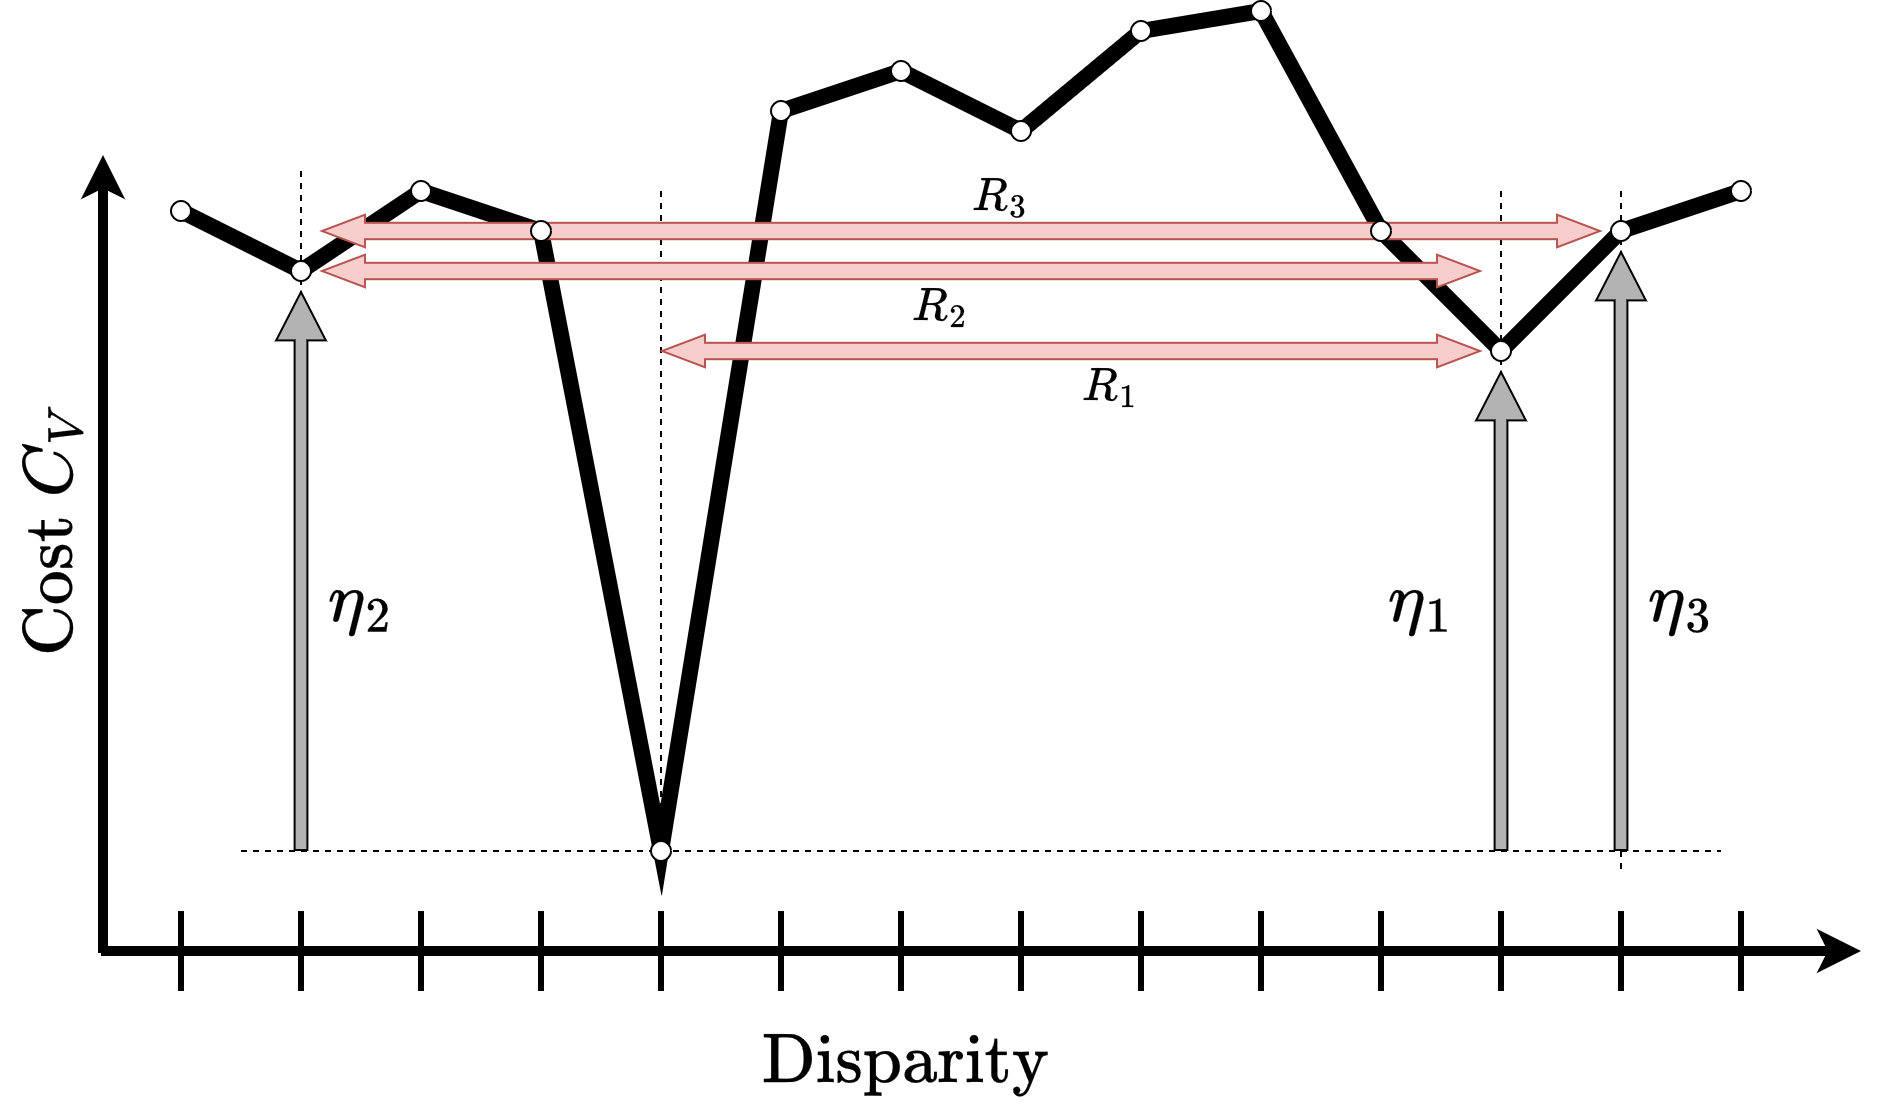
\includegraphics[width=\linewidth]{Images/Chap_1/Integral_Risk_1.png}
            \caption{Cost curve with different values of $\eta$ and risk}
            \label{fig:integral_risk_1}
        \end{subfigure}\hfill
        \begin{subfigure}[t]{0.4\linewidth}
            \centering
            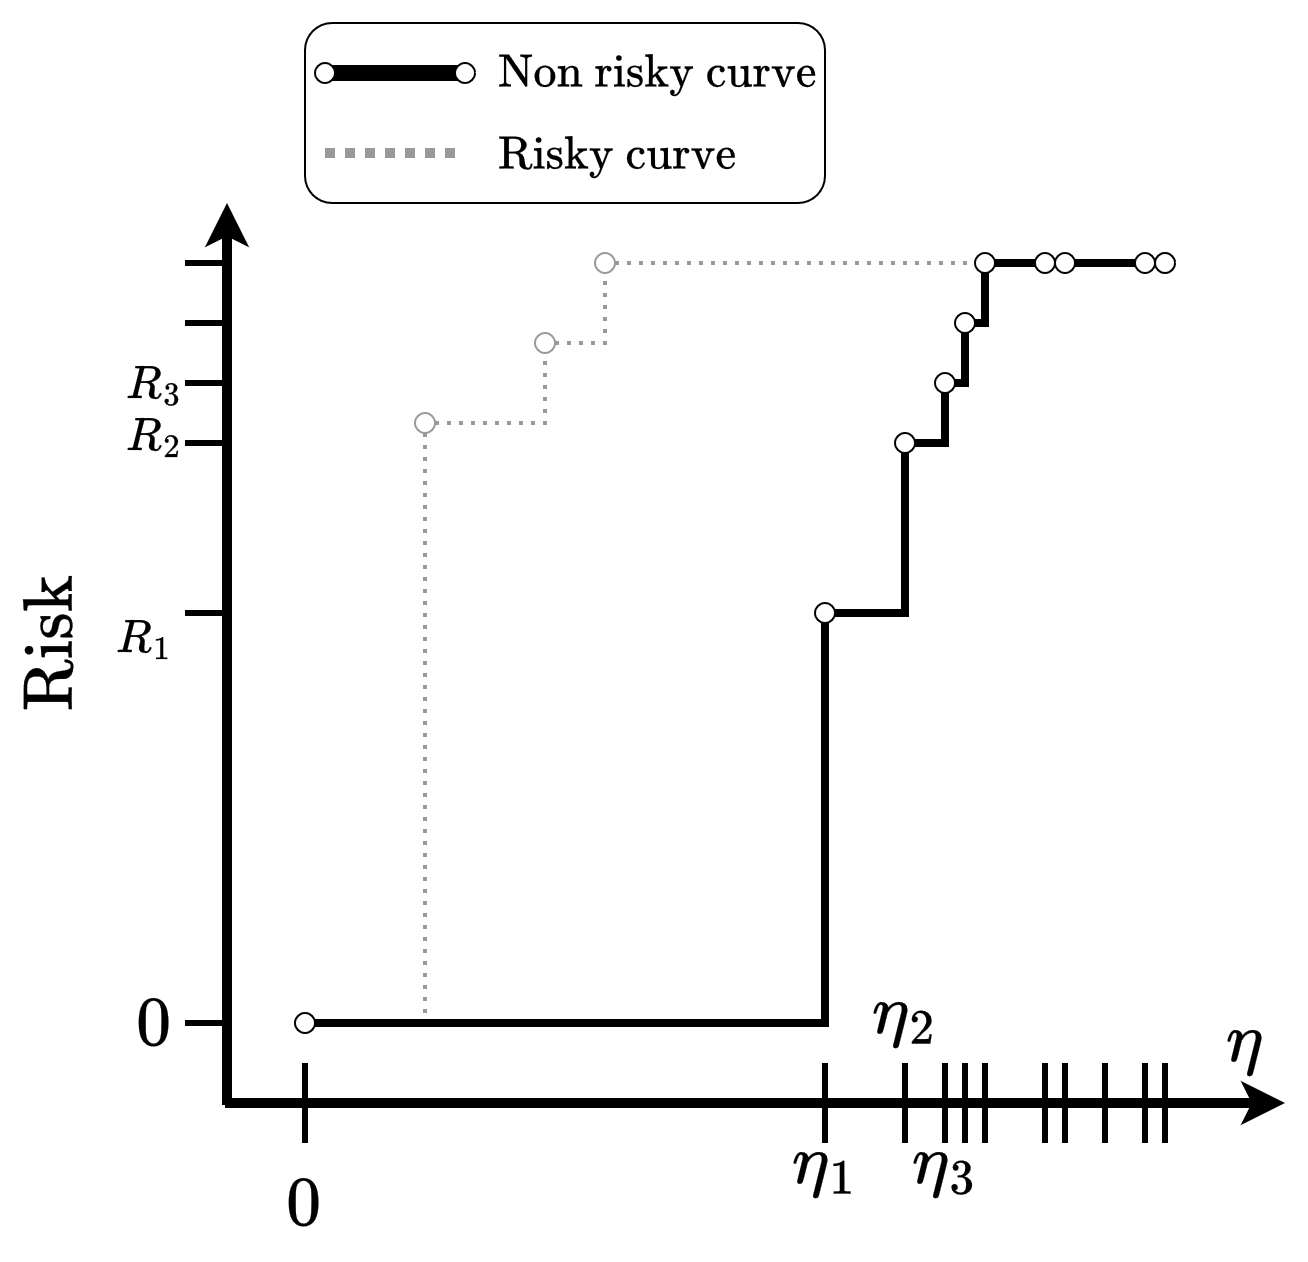
\includegraphics[width=\linewidth]{Images/Chap_1/Integral_Risk_2.png}
            \caption{Associated risk curve in full line. Risky curve in gray dotted line}
            \label{fig:integral_risk_2}
        \end{subfigure}\hfill
        \caption{Illustration of the computation of the risk curve.}
        \label{fig:integral_risk}
    \end{figure}
\end{comment}

The confidence from ambiguity, like other confidence measures, is designed to indicate potentially wrong matches. It however does not measure the extent of the potential error. After all, it is possible that we predict a wrong disparity, while the correct disparity is right next to our prediction. The impact of this error on the final result will be smaller than if the true disparity is at the other side of the disparity range. There is the a distinction to be made between the value of a confidence measures and the magnitude of a potential error, even if they can be correlated in some cases.

In \Cref{chap:epistemic_uncertainty,chap:elevation_intervals}, we introduce a method for computing confidence intervals, which aims to serve as a complement to confidence measures as it estimates the magnitude of the potential error. This method was motivated following discussions with different users and experts in 3D modelling from the AI4GEO consortium (\url{https://www.ai4geo.eu/}). Indeed, a common point that emerged from those discussions was the desire to produce confidence intervals alongside photogrammetry \acrshort{dsm}s. This also converged with the quality map requirement of the \acrshort{co3d} mission. We therefore developed our method with the objective of answering to this user need. This chapter presented the different concepts relative to satellite photogrammetry, and the different uncertainty associated with a photogrammetry pipeline. In the following, \Cref{chap:representation_of_uncertainty,chap:joining_credal_sets} will present relevant uncertainty models and concepts for this thesis, while \Cref{chap:propagating,chap:epistemic_uncertainty,chap:elevation_intervals} estimate the uncertainty at different steps of the photogrammetry pipeline.

\pagebreak
\blankpage
